%\documentclass[table]{article}
%\usepackage{beamerarticle}
\documentclass[10pt,xcolor=table,ignorenonframetext,handout,aspectratio=169]{beamer}
%\documentclass[10pt,xcolor=table,ignorenonframetext]{beamer}
\mode<presentation>
{
  \usetheme{default}
  \useoutertheme{split}
% \usefonttheme{serif}
}

\usenavigationsymbolstemplate{}
\usepackage{amssymb}
\usepackage{amsmath}
\usepackage{setspace}
\usepackage{graphicx}
\usepackage{multirow}
\usepackage[english]{babel}
\usepackage[latin1]{inputenc}
\usepackage{bm}
\usepackage{graphicx}
\usepackage{multirow}
\usepackage{tikz}
\usepackage[english]{babel}
\usepackage[latin1]{inputenc}
%\usepackage{ulem}
\usepackage{pifont}
\usepackage{changepage}
%\usepackage{colortbl}
%\usepackage[table]{xcolor}
%\usepackage{xcolor}

\setbeamersize{text margin left=1cm,text margin right=5cm}

\setbeamertemplate{itemize item}[circle]
\setbeamertemplate{frametitle}[default][center]

\newlength{\wideitemsep}
\setlength{\wideitemsep}{\itemsep}
\addtolength{\wideitemsep}{4pt}
\let\olditem\item
\renewcommand{\item}{\setlength{\itemsep}{\wideitemsep}\olditem}

\newcommand{\HRule}{\rule{0.5\textwidth}{0.05mm}}

\usetikzlibrary{arrows,positioning,shapes}
\usetikzlibrary{decorations.pathreplacing}
\usetikzlibrary{snakes}

\definecolor{blueish}{RGB}{97,156,255}
\definecolor{greenish}{RGB}{0,186,56}
\definecolor{reddish}{RGB}{248,118,109}

\definecolor{oiverm}{RGB}{213,94,0}
\definecolor{oiblue}{RGB}{0,114,178}
\definecolor{oigreen}{RGB}{0,158,115}
\definecolor{oipurple}{RGB}{204,121,167}
\definecolor{oiorange}{RGB}{230,159,0}
\definecolor{oisky}{RGB}{86,180,233}
\definecolor{oiyellow}{RGB}{240,228,66}
\definecolor{williams}{RGB}{81,38,152}

\definecolor{hue1}{RGB}{255,255,204}
\definecolor{hue2}{RGB}{161,218,180}
\definecolor{hue3}{RGB}{65,182,196}
\definecolor{hue4}{RGB}{44,127,184}
\definecolor{hue5}{RGB}{37,52,148}

\definecolor{dvg1}{RGB}{213,62,79}
\definecolor{dvg2}{RGB}{244,109,67}
\definecolor{dvg3}{RGB}{253,174,97}
\definecolor{dvg4}{RGB}{254,224,139}
\definecolor{dvg5}{RGB}{230,245,152}
\definecolor{dvg6}{RGB}{171,221,164}
\definecolor{dvg7}{RGB}{102,194,165}
\definecolor{dvg8}{RGB}{50,136,189}

\setbeamercolor{structure}{fg=williams,bg=williams!12}

\title{Two-Way Fixed Effects, Slide \insertframenumber}
\subtitle{}

\author{Economics 379 (Professor Jakiela)}
\date{}



\begin{document}
	
	
	
%%%%%%%%%%%%%%%%%%%%%%%%%%%%%%%%%%%%%%%%%%%%%%%%%%%%%%%%%%%%%%%%%%%%%%%%%%
	% COURSE Title slide
%%%%%%%%%%%%%%%%%%%%%%%%%%%%%%%%%%%%%%%%%%%%%%%%%%%%%%%%%%%%%%%%%%%%%%%%%%
	
\begin{frame}<beamer:0>[plain]
	
	\begin{center}
		\begin{tikzpicture}
		
		\node [opacity=1] (bg)  {\includegraphics[keepaspectratio,height=0.9\paperheight]{photos/Kenya-cistern-Flore-de-Preneuf-2011-LARGE.jpg}};
		
		\node [anchor=east,align=right] at (6,-2.25) {\Large{\textcolor{white}{Williams College ECON 379:}}};		
		\node [anchor=east,align=right] at (6,-3) {\Large{\textcolor{white}{Program Evaluation for International Development}}};

		\node [anchor=east] at (6,-3.8) {\textcolor{yellow}{\tiny{photo:  Flore de Preneuf / World Bank}}};
		
		\end{tikzpicture}
	\end{center}
\end{frame}


%%%%%%%%%%%%%%%%%%%%%%%%%%%%%%%%%%%%%%%%%%%%%%%%%%%%%%%%%%%%%%%%%%%%%%%%%%
% LECTURE Title slide
%%%%%%%%%%%%%%%%%%%%%%%%%%%%%%%%%%%%%%%%%%%%%%%%%%%%%%%%%%%%%%%%%%%%%%%%%%

\begin{frame}[plain]

\only<beamer>{\begin{adjustwidth}{0cm}{-4cm}}

\begin{center}
	\begin{tikzpicture}
	
	\node [opacity=0.25] (bg)  {\includegraphics[keepaspectratio,height=0.9\paperheight]{photos/Senegal-WAAPP-seeds-Daniella-Van-Leggelo-Padilla-LARGE.jpg}};
	
	\node at (0,2.5) {\large{\textcolor{williams}{Williams College ECON 379:}}};		
	\node at (0,1.5) {\large{\textcolor{williams}{Program Evaluation for International Development}}};
	
	\node at (0,-0.5) {\large{\textcolor{williams}{\textbf{Module 7: Two-Way Fixed Effects}}}};
	
	\node at (0,-2) {\large{\textcolor{williams}{Professor:  Pamela Jakiela}}};
	
	\node [anchor=east] at (6,-3.8) {\textcolor{yellow}{\tiny{photo:  Daniella Van Leggelo-Padilla / World Bank}}};
	
	\end{tikzpicture}
\end{center}
\only<beamer>{\end{adjustwidth}}
\end{frame}



%%%%%%%%%%%%%%%%%%%%%%%%%%%%%%%%%%%%%%%%%%%%%%%%%%%%%%%%%%%%%%%%%%%%%%%%%%%

%\begin{frame}<handout:0>[bg,plain]
\begin{frame}[plain]

\only<beamer>{\begin{adjustwidth}{0cm}{-4cm}}
	
	\begin{center}
		
		%\Large{\textcolor{white}{Budget Sets and Budget Lines}}
		\Large{\textcolor{williams}{Diff-in-Diff with Staggered Timing}}
		
	\end{center}
	
	\only<beamer>{\end{adjustwidth}}
\end{frame}


%%%%%%%%%%%%%%%%%%%%%%%%%%%%%%%%%%%%%%%%%%%%%%%%%%%%%%%%%%%%%%%%%%%%%%%%%%%%%%%%%%

\newpage
\begin{frame}{Variation in Treatment Timing}

\medskip

\textbf{Example:}  counties introduced food stamps at different times

\medskip
\medskip

\begin{center}

\begin{tabular}{cc}
	\includegraphics[height=3.2cm]{img/AlmondEtAl-graph.png}
	& 
	\includegraphics[height=3.2cm]{img/AlmondEtAl-map.png} \\
\end{tabular}

\smallskip

\tiny{\textcolor{gray}{source:  Almond, Hoynes, and Schanzenbach (AER, 2016)}}
\end{center}



\end{frame}


%%%%%%%%%%%%%%%%%%%%%%%%%%%%%%%%%%%%%%%%%%%%%%%%%%%%%%%%%%%%%%%%%%%%%%%%%%%%%%%%%%

\newpage
\begin{frame}{Variation in Treatment Timing}

\medskip

\begin{center}

\textbf{Example:}  states adopted Medicaid at different times

\medskip	
\medskip

\includegraphics[height=4.8cm]{img/BoudreauxEtAl-map.png} 

\smallskip

\tiny{\textcolor{gray}{source:  Boudreaux, Golberstein, and McAlpine (Journal of Health Economics, 2016)}}
\end{center}



\end{frame}


%%%%%%%%%%%%%%%%%%%%%%%%%%%%%%%%%%%%%%%%%%%%%%%%%%%%%%%%%%%%%%%%%%%%%%%%%%%%%%%%%%

\newpage
\begin{frame}{Variation in Treatment Timing}

\medskip

\begin{center}

\textbf{Example:}  counties opening community health centers

\medskip
\medskip

\includegraphics[height=4.8cm]{img/BaileyGoodmanBacon-map.png} 

\smallskip

\tiny{\textcolor{gray}{source:  Bailey and Goodman-Bacon (AER, 2015)}}
\end{center}

\end{frame}


%%%%%%%%%%%%%%%%%%%%%%%%%%%%%%%%%%%%%%%%%%%%%%%%%%%%%%%%%%%%%%%%%%%%%%%%%%%%%%%%%%

\newpage
\begin{frame}{Variation in Treatment Timing}

\medskip

\begin{center}

\textbf{Example:}  African countries democratized at different times

\medskip
\medskip

\includegraphics[height=4.8cm]{img/Kudamatsu-map.pdf} 

\smallskip

\tiny{\textcolor{gray}{source:  Kudamatsu (JEEA, 2012)}}
\end{center}

\end{frame}


%%%%%%%%%%%%%%%%%%%%%%%%%%%%%%%%%%%%%%%%%%%%%%%%%%%%%%%%%%%%%%%%%%%%%%%%%%%%%%%%%%

\newpage
\begin{frame}<handout:0>{Two-Way Fixed Effects Estimates of $\beta^{DD}$}

\begin{center}
\begin{tikzpicture}

% blank canvas
\only<handout>{\fill[fill=white,draw=white,ultra thin]
(0,0) -- (11,0) -- (11,6) -- (0,6) -- cycle;}
\only<beamer>{\fill[fill=white,draw=white,ultra thin]
(0,0) -- (14,0) -- (14,6) -- (0,6) -- cycle;}
\only<beamer>{\draw[draw=oiblue!60,fill=oiblue!10,opacity=0.5] (11,1) rectangle (14,5);}
%\draw[step=1.0,gray!20,thin] (0,0) grid (11,6);

%	\pgfmathsetmacro\xshift{0.5cm};
%	\pgfmathsetmacro\yshift{5.5cm};
%	\pgfmathsetmacro\mycolor{"gray"};

\node (eq1) at (5,3.5) {$+$};

\node [anchor=base east, align=right] (eq1A) at ([xshift=0.125cm]eq1.base west) {$\gamma_t$};
\node [anchor=base east, align=right] (eq1B) at ([xshift=0.125cm]eq1A.base west) {$+$};
\node [anchor=base east, align=right] (eq1C) at ([xshift=0.125cm]eq1B.base west) {$\alpha_i$};
\node [anchor=base east, align=right] (eq1D) at ([xshift=0.125cm]eq1C.base west) {$=$};
\node [anchor=base east, align=right] (eq1E) at ([xshift=0.125cm]eq1D.base west) {$Y_{it}$};

\node [anchor=base west, align=right] (eq1ZZ) at ([xshift=-0.125cm]eq1.base east) {$\beta^{DD}$};	
\node [anchor=base west, align=right] (eq1Z) at ([xshift=-0.25cm]eq1ZZ.base east) {$D_{it}$};
\node [anchor=base west, align=right] (eq1Y) at ([xshift=-0.125cm]eq1Z.base east) {$+$};
\node [anchor=base west, align=right] (eq1X) at ([xshift=-0.125cm]eq1Y.base east) {$\varepsilon_{it}$};

\end{tikzpicture}
\end{center}

\end{frame}



%%%%%%%%%%%%%%%%%%%%%%%%%%%%%%%%%%%%%%%%%%%%%%%%%%%%%%%%%%%%%%%%%%%%%%%%%%%%%%%%%%

\newpage
\begin{frame}<handout:0>{Two-Way Fixed Effects Estimates of $\beta^{DD}$}

\begin{center}
\begin{tikzpicture}

% blank canvas
\only<handout>{\fill[fill=white,draw=white,ultra thin]
(0,0) -- (11,0) -- (11,6) -- (0,6) -- cycle;}
\only<beamer>{\fill[fill=white,draw=white,ultra thin]
(0,0) -- (14,0) -- (14,6) -- (0,6) -- cycle;}
\only<beamer>{\draw[draw=oiblue!60,fill=oiblue!10,opacity=0.5] (11,1) rectangle (14,5);}
%\draw[step=1.0,gray!20,thin] (0,0) grid (11,6);

%	\pgfmathsetmacro\xshift{0.5cm};
%	\pgfmathsetmacro\yshift{5.5cm};
%	\pgfmathsetmacro\mycolor{"gray"};

\node (eq1) at (5,3.5) {$+$};

\node [oiblue,anchor=base east, align=right] (eq1A) at ([xshift=0.125cm]eq1.base west) {$\gamma_t$};
\node [anchor=base east, align=right] (eq1B) at ([xshift=0.125cm]eq1A.base west) {$+$};
\node [oiblue,anchor=base east, align=right] (eq1C) at ([xshift=0.125cm]eq1B.base west) {$\alpha_i$};
\node [anchor=base east, align=right] (eq1D) at ([xshift=0.125cm]eq1C.base west) {$=$};
\node [anchor=base east, align=right] (eq1E) at ([xshift=0.125cm]eq1D.base west) {$Y_{it}$};

\node [anchor=base west, align=right] (eq1ZZ) at ([xshift=-0.125cm]eq1.base east) {$\beta^{DD}$};	
\node [anchor=base west, align=right] (eq1Z) at ([xshift=-0.25cm]eq1ZZ.base east) {$D_{it}$};
\node [anchor=base west, align=right] (eq1Y) at ([xshift=-0.125cm]eq1Z.base east) {$+$};
\node [anchor=base west, align=right] (eq1X) at ([xshift=-0.125cm]eq1Y.base east) {$\varepsilon_{it}$};

\node[oiblue,anchor=north,align=center] (lbl1) at ([yshift=-1.5cm]eq1A.south) {time fixed effects};
\draw[oiblue,->] (lbl1.north) -- (eq1A.south);

\node[oiblue,anchor=north,align=center] (lbl2) at ([xshift=-2cm,yshift=-0.75cm]eq1C.south) {unit fixed effects};
\draw[oiblue,->] (lbl2.north east) -- ([xshift=-0.05cm]eq1C.south);

\end{tikzpicture}
\end{center}

\end{frame}


%%%%%%%%%%%%%%%%%%%%%%%%%%%%%%%%%%%%%%%%%%%%%%%%%%%%%%%%%%%%%%%%%%%%%%%%%%%%%%%%%%

\newpage
\begin{frame}<handout:0>{Two-Way Fixed Effects Estimates of $\beta^{DD}$}

\begin{center}
\begin{tikzpicture}

% blank canvas
\only<handout>{\fill[fill=white,draw=white,ultra thin]
(0,0) -- (11,0) -- (11,6) -- (0,6) -- cycle;}
\only<beamer>{\fill[fill=white,draw=white,ultra thin]
(0,0) -- (14,0) -- (14,6) -- (0,6) -- cycle;}
\only<beamer>{\draw[draw=oiblue!60,fill=oiblue!10,opacity=0.5] (11,1) rectangle (14,5);}
%\draw[step=1.0,gray!20,thin] (0,0) grid (11,6);

%	\pgfmathsetmacro\xshift{0.5cm};
%	\pgfmathsetmacro\yshift{5.5cm};
%	\pgfmathsetmacro\mycolor{"gray"};

\node (eq1) at (5,3.5) {$+$};

\node [oiblue,anchor=base east, align=right] (eq1A) at ([xshift=0.125cm]eq1.base west) {$\gamma_t$};
\node [anchor=base east, align=right] (eq1B) at ([xshift=0.125cm]eq1A.base west) {$+$};
\node [oiblue,anchor=base east, align=right] (eq1C) at ([xshift=0.125cm]eq1B.base west) {$\alpha_i$};
\node [anchor=base east, align=right] (eq1D) at ([xshift=0.125cm]eq1C.base west) {$=$};
\node [anchor=base east, align=right] (eq1E) at ([xshift=0.125cm]eq1D.base west) {$Y_{it}$};

\node [anchor=base west, align=right] (eq1ZZ) at ([xshift=-0.125cm]eq1.base east) {$\beta^{DD}$};	
\node [oiverm,anchor=base west, align=right] (eq1Z) at ([xshift=-0.25cm]eq1ZZ.base east) {$D_{it}$};
\node [anchor=base west, align=right] (eq1Y) at ([xshift=-0.125cm]eq1Z.base east) {$+$};
\node [anchor=base west, align=right] (eq1X) at ([xshift=-0.125cm]eq1Y.base east) {$\varepsilon_{it}$};

\node[oiblue,anchor=north,align=center] (lbl1) at ([yshift=-1.5cm]eq1A.south) {time fixed effects};
\draw[oiblue,->] (lbl1.north) -- (eq1A.south);

\node[oiblue,anchor=north,align=center] (lbl2) at ([xshift=-2cm,yshift=-0.75cm]eq1C.south) {unit fixed effects};
\draw[oiblue,->] (lbl2.north east) -- ([xshift=-0.05cm]eq1C.south);

\node[oiverm,anchor=north,align=center] (lbl3) at ([xshift=2cm,yshift=-0.75cm]eq1Z.south) {\textbf{treatment dummy}};	
\draw[oiverm,->] (lbl3.north west) -- ([xshift=0.05cm]eq1Z.south);

\node[oiverm!72,anchor=north,align=center,text width = 3.2cm] (lbl3B) at ([yshift=0cm]lbl3.south) {that turns ``on'' at \\
different times };

\end{tikzpicture}
\end{center}

\end{frame}



%%%%%%%%%%%%%%%%%%%%%%%%%%%%%%%%%%%%%%%%%%%%%%%%%%%%%%%%%%%%%%%%%%%%%%%%%%%%%%%%%%

\newpage
\begin{frame}{Two-Way Fixed Effects Estimates of $\beta^{DD}$}

\begin{center}
\begin{tikzpicture}

% blank canvas
\only<handout>{\fill[fill=white,draw=white,ultra thin]
(0,0) -- (11,0) -- (11,6) -- (0,6) -- cycle;}
\only<beamer>{\fill[fill=white,draw=white,ultra thin]
(0,0) -- (14,0) -- (14,6) -- (0,6) -- cycle;}
\only<beamer>{\draw[draw=oiblue!60,fill=oiblue!10,opacity=0.5] (11,1) rectangle (14,5);}
%\draw[step=1.0,gray!20,thin] (0,0) grid (11,6);

%	\pgfmathsetmacro\xshift{0.5cm};
%	\pgfmathsetmacro\yshift{5.5cm};
%	\pgfmathsetmacro\mycolor{"gray"};

\node (eq1) at (5,3.5) {$+$};

\node [anchor=base east, align=right] (eq1A) at ([xshift=0.125cm]eq1.base west) {$\gamma_t$};
\node [anchor=base east, align=right] (eq1B) at ([xshift=0.125cm]eq1A.base west) {$+$};
\node [anchor=base east, align=right] (eq1C) at ([xshift=0.125cm]eq1B.base west) {$\alpha_i$};
\node [anchor=base east, align=right] (eq1D) at ([xshift=0.125cm]eq1C.base west) {$=$};
\node [anchor=base east, align=right] (eq1E) at ([xshift=0.125cm]eq1D.base west) {$Y_{it}$};

\node [red,anchor=base west, align=right] (eq1ZZ) at ([xshift=-0.125cm]eq1.base east) {$\beta^{DD}$};	
\node [anchor=base west, align=right] (eq1Z) at ([xshift=-0.25cm]eq1ZZ.base east) {$D_{it}$};
\node [anchor=base west, align=right] (eq1Y) at ([xshift=-0.125cm]eq1Z.base east) {$+$};
\node [anchor=base west, align=right] (eq1X) at ([xshift=-0.125cm]eq1Y.base east) {$\varepsilon_{it}$};

\node[gray,anchor=north,align=center] (lbl1) at ([yshift=-1.5cm]eq1A.south) {time fixed effects};
\draw[gray,->] (lbl1.north) -- (eq1A.south);

\node[gray,anchor=north,align=center] (lbl2) at ([xshift=-2cm,yshift=-0.75cm]eq1C.south) {unit fixed effects};
\draw[gray,->] (lbl2.north east) -- ([xshift=-0.05cm]eq1C.south);

\node[gray,anchor=north,align=center] (lbl3) at ([xshift=2cm,yshift=-0.75cm]eq1Z.south) {\textbf{treatment dummy}};	
\draw[gray,->] (lbl3.north west) -- ([xshift=0.05cm]eq1Z.south);

\node[gray!72,anchor=north,align=center,text width = 3.2cm] (lbl3B) at ([yshift=0cm]lbl3.south) {that turns ``on'' at \\
different times };

\node[red,anchor=south,align=center] (lbl4) at ([yshift=1.0cm]eq1ZZ.north) {What exactly is $\beta^{DD}$?};
\draw[red,->] (lbl4.south) -- (eq1ZZ.north);

\end{tikzpicture}
\end{center}

\end{frame}


%%%%%%%%%%%%%%%%%%%%%%%%%%%%%%%%%%%%%%%%%%%%%%%%%%%%%%%%%%%%%%%%%%%%%%%%%%%%%%%%%%

\newpage
\begin{frame}<handout:0>{What exactly is $\beta^{DD}$ in TWFE?}

\begin{center}
\begin{tikzpicture}

% blank canvas
\only<handout>{\fill[fill=white,draw=white,ultra thin]
(0,0) -- (11,0) -- (11,6) -- (0,6) -- cycle;}
\only<beamer>{\fill[fill=white,draw=white,ultra thin]
(0,0) -- (14,0) -- (14,6) -- (0,6) -- cycle;}
\only<beamer>{\draw[draw=oiblue!60,fill=oiblue!10,opacity=0.5] (11,1) rectangle (14,5);}
%\draw[step=1.0,gray!20,thin] (0,0) grid (11,6);

\filldraw[oiblue!48,opacity=0.32] (0.625,3) -- (0.625,4) -- (6.5,4) -- (6.5,3) -- cycle;

\foreach \y in {1,2,3,4} 
{
\pgfmathsetmacro\mylat{4.25 - 0.5*\y}
\node[font=\footnotesize,anchor=east,align=right] at (1.5,\mylat) {ID \y};
\pgfmathsetmacro\myline{4 - 0.5*\y}
\draw [gray!64] (0.625,\myline) -- (6.5,\myline);
}
\draw [gray!64] (0.625,4) -- (6.5,4);

\foreach \x in {2,3,4,5,6} 
{
\pgfmathtruncatemacro\label{\x - 1}
\pgfmathsetmacro\myline{\x - 0.5}
\node[font=\footnotesize,anchor=base,align=center] at (\x,4.125) {$t = \label$};
\draw [gray!64] (\myline,2) -- (\myline,4.5);
}
\draw [gray!64] (6.5,2) -- (6.5,4.5);

\foreach \x in {1,2} 
{
\foreach \y in {1,2,3,4} 
{
\pgfmathtruncatemacro\period{\x + 1}
\pgfmathsetmacro\mylat{4.25 - 0.5*\y}
\node[font=\footnotesize,anchor=center,align=center] at (\period,\mylat) {$0$};
}
}

\foreach \x in {3,4,5} 
{
\foreach \y in {1,2} 
{
\pgfmathtruncatemacro\period{\x + 1}
\pgfmathsetmacro\mylat{4.25 - 0.5*\y}
\node[font=\footnotesize,anchor=center,align=center] at (\period,\mylat) {$1$};
}
\foreach \y in {3,4} 
{
\pgfmathtruncatemacro\period{\x + 1}
\pgfmathsetmacro\mylat{4.25 - 0.5*\y}
\node[font=\footnotesize,anchor=center,align=center] at (\period,\mylat) {$0$};
}
}

\node[oiblue,anchor=west,align=left] at (6.5,3.5) {treatment};
\node[gray,anchor=west,align=left] at (6.5,2.5) {comparison};

\end{tikzpicture}
\end{center}

\end{frame}


%%%%%%%%%%%%%%%%%%%%%%%%%%%%%%%%%%%%%%%%%%%%%%%%%%%%%%%%%%%%%%%%%%%%%%%%%%%%%%%%%%

\newpage
\begin{frame}<handout:0>{What exactly is $\beta^{DD}$ in TWFE?}

\begin{center}
\begin{tikzpicture}

% blank canvas
\only<handout>{\fill[fill=white,draw=white,ultra thin]
(0,0) -- (11,0) -- (11,6) -- (0,6) -- cycle;}
\only<beamer>{\fill[fill=white,draw=white,ultra thin]
(0,0) -- (14,0) -- (14,6) -- (0,6) -- cycle;}
\only<beamer>{\draw[draw=oiblue!60,fill=oiblue!10,opacity=0.5] (11,1) rectangle (14,5);}
%\draw[step=1.0,gray!20,thin] (0,0) grid (11,6);

\filldraw[oiblue!48,opacity=0.32] (0.625,3) -- (0.625,4) -- (6.5,4) -- (6.5,3) -- cycle;
\filldraw[reddish!32,opacity=0.48] (3.5,2) -- (3.5,4.5) -- (6.5,4.5) -- (6.5,2) -- cycle;

\foreach \y in {1,2,3,4} 
{
\pgfmathsetmacro\mylat{4.25 - 0.5*\y}
\node[font=\footnotesize,anchor=east,align=right] at (1.5,\mylat) {ID \y};
\pgfmathsetmacro\myline{4 - 0.5*\y}
\draw [gray!64] (0.625,\myline) -- (6.5,\myline);
}
\draw [gray!64] (0.625,4) -- (6.5,4);

\foreach \x in {2,3,4,5,6} 
{
\pgfmathtruncatemacro\label{\x - 1}
\pgfmathsetmacro\myline{\x - 0.5}
\node[font=\footnotesize,anchor=base,align=center] at (\x,4.125) {$t = \label$};
\draw [gray!64] (\myline,2) -- (\myline,4.5);
}
\draw [gray!64] (6.5,2) -- (6.5,4.5);

\foreach \x in {1,2} 
{
\foreach \y in {1,2,3,4} 
{
\pgfmathtruncatemacro\period{\x + 1}
\pgfmathsetmacro\mylat{4.25 - 0.5*\y}
\node[font=\footnotesize,anchor=center,align=center] at (\period,\mylat) {$0$};
}
}

\foreach \x in {3,4,5} 
{
\foreach \y in {1,2} 
{
\pgfmathtruncatemacro\period{\x + 1}
\pgfmathsetmacro\mylat{4.25 - 0.5*\y}
\node[font=\footnotesize,anchor=center,align=center] at (\period,\mylat) {$1$};
}
\foreach \y in {3,4} 
{
\pgfmathtruncatemacro\period{\x + 1}
\pgfmathsetmacro\mylat{4.25 - 0.5*\y}
\node[font=\footnotesize,anchor=center,align=center] at (\period,\mylat) {$0$};
}
}

\node[oiblue,anchor=west,align=left] at (6.5,3.5) {treatment};
\node[gray,anchor=west,align=left] at (6.5,2.5) {comparison};

\end{tikzpicture}
\end{center}

\end{frame}



%%%%%%%%%%%%%%%%%%%%%%%%%%%%%%%%%%%%%%%%%%%%%%%%%%%%%%%%%%%%%%%%%%%%%%%%%%%%%%%%%%

\newpage
\begin{frame}{What exactly is $\beta^{DD}$ in TWFE?}

\begin{center}
\begin{tikzpicture}

% blank canvas
\only<handout>{\fill[fill=white,draw=white,ultra thin]
(0,0) -- (11,0) -- (11,6) -- (0,6) -- cycle;}
\only<beamer>{\fill[fill=white,draw=white,ultra thin]
(0,0) -- (14,0) -- (14,6) -- (0,6) -- cycle;}
\only<beamer>{\draw[draw=oiblue!60,fill=oiblue!10,opacity=0.5] (11,1) rectangle (14,5);}
%\draw[step=1.0,gray!20,thin] (0,0) grid (11,6);

\filldraw[oiblue!48,opacity=0.32] (0.625,3) -- (0.625,4) -- (6.5,4) -- (6.5,3) -- cycle;
\filldraw[reddish!32,opacity=0.48] (3.5,2) -- (3.5,4.5) -- (6.5,4.5) -- (6.5,2) -- cycle;

\foreach \y in {1,2,3,4} 
{
\pgfmathsetmacro\mylat{4.25 - 0.5*\y}
\node[font=\footnotesize,anchor=east,align=right] at (1.5,\mylat) {ID \y};
\pgfmathsetmacro\myline{4 - 0.5*\y}
\draw [gray!64] (0.625,\myline) -- (6.5,\myline);
}
\draw [gray!64] (0.625,4) -- (6.5,4);

\foreach \x in {2,3,4,5,6} 
{
\pgfmathtruncatemacro\label{\x - 1}
\pgfmathsetmacro\myline{\x - 0.5}
\node[font=\footnotesize,anchor=base,align=center] at (\x,4.125) {$t = \label$};
\draw [gray!64] (\myline,2) -- (\myline,4.5);
}
\draw [gray!64] (6.5,2) -- (6.5,4.5);

\foreach \x in {1,2} 
{
\foreach \y in {1,2} 
{
\pgfmathtruncatemacro\period{\x + 1}
\pgfmathsetmacro\mylat{4.25 - 0.5*\y}
\node[font=\footnotesize,anchor=center,align=center] at (\period,\mylat) {$3$};
}

\foreach \y in {3,4} 
{
\pgfmathtruncatemacro\period{\x + 1}
\pgfmathsetmacro\mylat{4.25 - 0.5*\y}
\node[font=\footnotesize,anchor=center,align=center] at (\period,\mylat) {$1$};
}
}

\foreach \x in {3,4,5} 
{
\foreach \y in {1,2} 
{
\pgfmathtruncatemacro\period{\x + 1}
\pgfmathsetmacro\mylat{4.25 - 0.5*\y}
\node[font=\footnotesize,anchor=center,align=center] at (\period,\mylat) {$5$};
}
\foreach \y in {3,4} 
{
\pgfmathtruncatemacro\period{\x + 1}
\pgfmathsetmacro\mylat{4.25 - 0.5*\y}
\node[font=\footnotesize,anchor=center,align=center] at (\period,\mylat) {$4$};
}
}

\node[oiblue,anchor=west,align=left] at (6.5,3.5) {treatment};
\node[gray,anchor=west,align=left] at (6.5,2.5) {comparison};

\node[red,anchor=west,align=left] at (1.5,1.5) {$\Rightarrow \beta^{DD} = \textcolor{red}{5} - 3 - \left( 4 - 1 \right)$};

\end{tikzpicture}
\end{center}

\end{frame}



%%%%%%%%%%%%%%%%%%%%%%%%%%%%%%%%%%%%%%%%%%%%%%%%%%%%%%%%%%%%%%%%%%%%%%%%%%%%%%%%%%

\newpage
\begin{frame}{What exactly is $\beta^{DD}$ in TWFE?}

\begin{center}
\begin{tikzpicture}

% blank canvas
\only<handout>{\fill[fill=white,draw=white,ultra thin]
(0,0) -- (11,0) -- (11,6) -- (0,6) -- cycle;}
\only<beamer>{\fill[fill=white,draw=white,ultra thin]
(0,0) -- (14,0) -- (14,6) -- (0,6) -- cycle;}
\only<beamer>{\draw[draw=oiblue!60,fill=oiblue!10,opacity=0.5] (11,1) rectangle (14,5);}
%\draw[step=1.0,gray!20,thin] (0,0) grid (11,6);

\filldraw[oiblue!48,opacity=0.32] (0.625,3) -- (0.625,4) -- (6.5,4) -- (6.5,3) -- cycle;
\filldraw[reddish!32,opacity=0.48] (3.5,2) -- (3.5,4.5) -- (6.5,4.5) -- (6.5,2) -- cycle;

\foreach \y in {1,2,3,4} 
{
\pgfmathsetmacro\mylat{4.25 - 0.5*\y}
\node[font=\footnotesize,anchor=east,align=right] at (1.5,\mylat) {ID \y};
\pgfmathsetmacro\myline{4 - 0.5*\y}
\draw [gray!64] (0.625,\myline) -- (6.5,\myline);
}
\draw [gray!64] (0.625,4) -- (6.5,4);

\foreach \x in {2,3,4,5,6} 
{
\pgfmathtruncatemacro\label{\x - 1}
\pgfmathsetmacro\myline{\x - 0.5}
\node[font=\footnotesize,anchor=base,align=center] at (\x,4.125) {$t = \label$};
\draw [gray!64] (\myline,2) -- (\myline,4.5);
}
\draw [gray!64] (6.5,2) -- (6.5,4.5);

\foreach \x in {1,2} 
{
\foreach \y in {1,2} 
{
\pgfmathtruncatemacro\period{\x + 1}
\pgfmathsetmacro\mylat{4.25 - 0.5*\y}
\node[font=\footnotesize,anchor=center,align=center] at (\period,\mylat) {$3$};
}

\foreach \y in {3,4} 
{
\pgfmathtruncatemacro\period{\x + 1}
\pgfmathsetmacro\mylat{4.25 - 0.5*\y}
\node[font=\footnotesize,anchor=center,align=center] at (\period,\mylat) {$1$};
}
}

\foreach \x in {3,4,5} 
{
\foreach \y in {1} 
{
\pgfmathtruncatemacro\period{\x + 1}
\pgfmathsetmacro\mylat{4.25 - 0.5*\y}
\node[red,font=\footnotesize,anchor=center,align=center] at (\period,\mylat) {$5$};
}
\foreach \y in {2} 
{
\pgfmathtruncatemacro\period{\x + 1}
\pgfmathsetmacro\mylat{4.25 - 0.5*\y}
\node[red,font=\footnotesize,anchor=center,align=center] at (\period,\mylat) {$7$};
}
\foreach \y in {3,4} 
{
\pgfmathtruncatemacro\period{\x + 1}
\pgfmathsetmacro\mylat{4.25 - 0.5*\y}
\node[font=\footnotesize,anchor=center,align=center] at (\period,\mylat) {$4$};
}
}

\node[oiblue,anchor=west,align=left] at (6.5,3.5) {treatment};
\node[gray,anchor=west,align=left] at (6.5,2.5) {comparison};

\node[anchor=west,align=left] (eq1) at (1.5,1.5) {$\Rightarrow \beta^{DD} = \textcolor{red}{6} - 3 - \left( 4 - 1 \right)$};
\node[red,anchor=base west,align=left] at (eq1.base east) {$\leftarrow $ average treatment effect};

\end{tikzpicture}
\end{center}

\end{frame}



%%%%%%%%%%%%%%%%%%%%%%%%%%%%%%%%%%%%%%%%%%%%%%%%%%%%%%%%%%%%%%%%%%%%%%%%%%%%%%%%%%

\newpage
\begin{frame}{Multiple Treatment and Comparison Groups}

\begin{center}
\begin{tikzpicture}

% blank canvas
\only<handout>{\fill[fill=white,draw=white,ultra thin]
(0,0) -- (11,0) -- (11,6) -- (0,6) -- cycle;}
\only<beamer>{\fill[fill=white,draw=white,ultra thin]
(0,0) -- (14,0) -- (14,6) -- (0,6) -- cycle;}
\only<beamer>{\draw[draw=oiblue!60,fill=oiblue!10,opacity=0.5] (11,1) rectangle (14,5);}
%\draw[step=1.0,gray!20,thin] (0,0) grid (11,6);

\filldraw[oiblue!48,opacity=0.32] (0.625,3) -- (0.625,4) -- (9.5,4) -- (9.5,3) -- cycle;
\filldraw[oiverm!48,opacity=0.32] (0.625,2) -- (0.625,3) -- (9.5,3) -- (9.5,2) -- cycle;
\filldraw[oiyellow!48,opacity=0.64] (0.625,1) -- (0.625,2) -- (9.5,2) -- (9.5,1) -- cycle;

\foreach \y in {1,2,3,4,5,6} 
{
\pgfmathsetmacro\mylat{4.25 - 0.5*\y}
\node[font=\footnotesize,anchor=east,align=right] at (1.5,\mylat) {ID \y};
\pgfmathsetmacro\myline{0.5 + 0.5*\y}
\draw [gray!64] (0.625,\myline) -- (9.5,\myline);
}
\draw [gray!64] (0.6255,4) -- (9.5,4);

\foreach \x in {2,3,4,5,6,7,8,9} 
{
\pgfmathtruncatemacro\label{\x - 1}
\pgfmathsetmacro\myline{\x - 0.5}
\node[font=\footnotesize,anchor=base,align=center] at (\x,4.125) {$t = \label$};
\draw [gray!64] (\myline,1) -- (\myline,4.5);
}
\draw [gray!64] (9.5,1) -- (9.5,4.5);

\foreach \x in {1,2} 
{
\foreach \y in {1,2,3,4,5,6} 
{
\pgfmathtruncatemacro\period{\x + 1}
\pgfmathsetmacro\mylat{4.25 - 0.5*\y}
\node[font=\footnotesize,anchor=center,align=center] at (\period,\mylat) {$0$};
}
}

\foreach \x in {3,4,5} 
{
\foreach \y in {1,2} 
{
\pgfmathtruncatemacro\period{\x + 1}
\pgfmathsetmacro\mylat{4.25 - 0.5*\y}
\node[font=\footnotesize,anchor=center,align=center] at (\period,\mylat) {$1$};
}
\foreach \y in {3,4,5,6} 
{
\pgfmathtruncatemacro\period{\x + 1}
\pgfmathsetmacro\mylat{4.25 - 0.5*\y}
\node[font=\footnotesize,anchor=center,align=center] at (\period,\mylat) {$0$};
}
}


\foreach \x in {6,7,8} 
{
\foreach \y in {1,2,3,4} 
{
\pgfmathtruncatemacro\period{\x + 1}
\pgfmathsetmacro\mylat{4.25 - 0.5*\y}
\node[font=\footnotesize,anchor=center,align=center] at (\period,\mylat) {$1$};
}
\foreach \y in {5,6} 
{
\pgfmathtruncatemacro\period{\x + 1}
\pgfmathsetmacro\mylat{4.25 - 0.5*\y}
\node[font=\footnotesize,anchor=center,align=center] at (\period,\mylat) {$0$};
}
}

\end{tikzpicture}
\end{center}

\end{frame}



%%%%%%%%%%%%%%%%%%%%%%%%%%%%%%%%%%%%%%%%%%%%%%%%%%%%%%%%%%%%%%%%%%%%%%%%%%%%%%%%%%

\newpage
\begin{frame}<handout:0>{Multiple Treatment and Comparison Groups}

\begin{center}
\begin{tikzpicture}

% blank canvas
\only<handout>{\fill[fill=white,draw=white,ultra thin]
(0,0) -- (11,0) -- (11,6) -- (0,6) -- cycle;}
\only<beamer>{\fill[fill=white,draw=white,ultra thin]
(0,0) -- (14,0) -- (14,6) -- (0,6) -- cycle;}
\only<beamer>{\draw[draw=oiblue!60,fill=oiblue!10,opacity=0.5] (11,1) rectangle (14,5);}
%\draw[step=1.0,gray!20,thin] (0,0) grid (11,6);

\filldraw[gray!32,opacity=0.48] (1.5,2) -- (1.5,4.5) -- (6.5,4.5) -- (6.5,2) -- cycle;
\filldraw[gray!32,opacity=0.48] (0.625,4) -- (0.625,2) -- (1.5,2) -- (1.5,4) -- cycle;
\filldraw[oiblue!48,opacity=0.32] (1.5,3) -- (1.5,4) -- (6.5,4) -- (6.5,3) -- cycle;
\filldraw[oiverm!48,opacity=0.32] (1.5,2) -- (1.55,3) -- (6.5,3) -- (6.5,2) -- cycle;
%\filldraw[oiyellow!48,opacity=0.64] (0.625,1) -- (0.625,2) -- (9.5,2) -- (9.5,1) -- cycle;\\


\foreach \y in {1,2,3,4,5,6} 
{
\pgfmathsetmacro\mylat{4.25 - 0.5*\y}
\node[font=\footnotesize,anchor=east,align=right] at (1.5,\mylat) {ID \y};
\pgfmathsetmacro\myline{0.5 + 0.5*\y}
\draw [gray!64] (0.625,\myline) -- (9.5,\myline);
}
\draw [gray!64] (0.6255,4) -- (9.5,4);

\foreach \x in {2,3,4,5,6,7,8,9} 
{
\pgfmathtruncatemacro\label{\x - 1}
\pgfmathsetmacro\myline{\x - 0.5}
\node[font=\footnotesize,anchor=base,align=center] at (\x,4.125) {$t = \label$};
\draw [gray!64] (\myline,1) -- (\myline,4.5);
}
\draw [gray!64] (9.5,1) -- (9.5,4.5);

\foreach \x in {1,2} 
{
\foreach \y in {1,2,3,4} 
{
\pgfmathtruncatemacro\period{\x + 1}
\pgfmathsetmacro\mylat{4.25 - 0.5*\y}
\node[font=\footnotesize,anchor=center,align=center] at (\period,\mylat) {$0$};
}
\foreach \y in {5,6} 
{
\pgfmathtruncatemacro\period{\x + 1}
\pgfmathsetmacro\mylat{4.25 - 0.5*\y}
\node[gray,font=\footnotesize,anchor=center,align=center] at (\period,\mylat) {$0$};
}
}

\foreach \x in {3,4,5} 
{
\foreach \y in {1,2} 
{
\pgfmathtruncatemacro\period{\x + 1}
\pgfmathsetmacro\mylat{4.25 - 0.5*\y}
\node[red,font=\footnotesize,anchor=center,align=center] at (\period,\mylat) {$1$};
}
\foreach \y in {3,4} 
{
\pgfmathtruncatemacro\period{\x + 1}
\pgfmathsetmacro\mylat{4.25 - 0.5*\y}
\node[font=\footnotesize,anchor=center,align=center] at (\period,\mylat) {$0$};
}
\foreach \y in {5,6} 
{
\pgfmathtruncatemacro\period{\x + 1}
\pgfmathsetmacro\mylat{4.25 - 0.5*\y}
\node[gray,font=\footnotesize,anchor=center,align=center] at (\period,\mylat) {$0$};
}
}


\foreach \x in {6,7,8} 
{
\foreach \y in {1,2,3,4} 
{
\pgfmathtruncatemacro\period{\x + 1}
\pgfmathsetmacro\mylat{4.25 - 0.5*\y}
\node[gray,font=\footnotesize,anchor=center,align=center] at (\period,\mylat) {$1$};
}
\foreach \y in {5,6} 
{
\pgfmathtruncatemacro\period{\x + 1}
\pgfmathsetmacro\mylat{4.25 - 0.5*\y}
\node[gray,font=\footnotesize,anchor=center,align=center] at (\period,\mylat) {$0$};
}
}

\end{tikzpicture}
\end{center}

\end{frame}



%%%%%%%%%%%%%%%%%%%%%%%%%%%%%%%%%%%%%%%%%%%%%%%%%%%%%%%%%%%%%%%%%%%%%%%%%%%%%%%%%%

\newpage
\begin{frame}<handout:0>{Multiple Treatment and Comparison Groups}

\begin{center}
\begin{tikzpicture}

% blank canvas
\only<handout>{\fill[fill=white,draw=white,ultra thin]
(0,0) -- (11,0) -- (11,6) -- (0,6) -- cycle;}
\only<beamer>{\fill[fill=white,draw=white,ultra thin]
(0,0) -- (14,0) -- (14,6) -- (0,6) -- cycle;}
\only<beamer>{\draw[draw=oiblue!60,fill=oiblue!10,opacity=0.5] (11,1) rectangle (14,5);}
%\draw[step=1.0,gray!20,thin] (0,0) grid (11,6);

\filldraw[gray!32,opacity=0.48] (3.5,1) -- (3.5,4.5) -- (9.5,4.5) -- (9.5,1) -- cycle;
\filldraw[gray!32,opacity=0.48] (0.625,3) -- (0.625,1) -- (3.5,1) -- (3.5,3) -- cycle;
\filldraw[oiverm!48,opacity=0.32] (1.5,2) -- (1.5,3) -- (9.5,3) -- (9.5,2) -- cycle;
\filldraw[oiyellow!48,opacity=0.64] (1.5,1) -- (1.5,2) -- (9.5,2) -- (9.5,1) -- cycle;


\foreach \y in {1,2,3,4,5,6} 
{
\pgfmathsetmacro\mylat{4.25 - 0.5*\y}
\node[font=\footnotesize,anchor=east,align=right] at (1.5,\mylat) {ID \y};
\pgfmathsetmacro\myline{0.5 + 0.5*\y}
\draw [gray!64] (0.625,\myline) -- (9.5,\myline);
}
\draw [gray!64] (0.6255,4) -- (9.5,4);

\foreach \x in {2,3,4,5,6,7,8,9} 
{
\pgfmathtruncatemacro\label{\x - 1}
\pgfmathsetmacro\myline{\x - 0.5}
\node[font=\footnotesize,anchor=base,align=center] at (\x,4.125) {$t = \label$};
\draw [gray!64] (\myline,1) -- (\myline,4.5);
}
\draw [gray!64] (9.5,1) -- (9.5,4.5);

\foreach \x in {1,2} 
{
\foreach \y in {1,2} 
{
\pgfmathtruncatemacro\period{\x + 1}
\pgfmathsetmacro\mylat{4.25 - 0.5*\y}
\node[gray,font=\footnotesize,anchor=center,align=center] at (\period,\mylat) {$0$};
}
\foreach \y in {3,4,5,6} 
{
\pgfmathtruncatemacro\period{\x + 1}
\pgfmathsetmacro\mylat{4.25 - 0.5*\y}
\node[font=\footnotesize,anchor=center,align=center] at (\period,\mylat) {$0$};
}
}

\foreach \x in {3,4,5} 
{
\foreach \y in {1,2} 
{
\pgfmathtruncatemacro\period{\x + 1}
\pgfmathsetmacro\mylat{4.25 - 0.5*\y}
\node[gray,font=\footnotesize,anchor=center,align=center] at (\period,\mylat) {$1$};
}
\foreach \y in {3,4} 
{
\pgfmathtruncatemacro\period{\x + 1}
\pgfmathsetmacro\mylat{4.25 - 0.5*\y}
\node[font=\footnotesize,anchor=center,align=center] at (\period,\mylat) {$0$};
}
\foreach \y in {5,6} 
{
\pgfmathtruncatemacro\period{\x + 1}
\pgfmathsetmacro\mylat{4.25 - 0.5*\y}
\node[font=\footnotesize,anchor=center,align=center] at (\period,\mylat) {$0$};
}
}


\foreach \x in {6,7,8} 
{
\foreach \y in {1,2} 
{
\pgfmathtruncatemacro\period{\x + 1}
\pgfmathsetmacro\mylat{4.25 - 0.5*\y}
\node[gray,font=\footnotesize,anchor=center,align=center] at (\period,\mylat) {$1$};
}
\foreach \y in {3,4} 
{
\pgfmathtruncatemacro\period{\x + 1}
\pgfmathsetmacro\mylat{4.25 - 0.5*\y}
\node[red,font=\footnotesize,anchor=center,align=center] at (\period,\mylat) {$1$};
}
\foreach \y in {5,6} 
{
\pgfmathtruncatemacro\period{\x + 1}
\pgfmathsetmacro\mylat{4.25 - 0.5*\y}
\node[font=\footnotesize,anchor=center,align=center] at (\period,\mylat) {$0$};
}
}

\end{tikzpicture}
\end{center}

\end{frame}



%%%%%%%%%%%%%%%%%%%%%%%%%%%%%%%%%%%%%%%%%%%%%%%%%%%%%%%%%%%%%%%%%%%%%%%%%%%%%%%%%%

\newpage
\begin{frame}<handout:0>{Multiple Treatment and Comparison Groups}

\begin{center}
\begin{tikzpicture}

% blank canvas
\only<handout>{\fill[fill=white,draw=white,ultra thin]
(0,0) -- (11,0) -- (11,6) -- (0,6) -- cycle;}
\only<beamer>{\fill[fill=white,draw=white,ultra thin]
(0,0) -- (14,0) -- (14,6) -- (0,6) -- cycle;}
\only<beamer>{\draw[draw=oiblue!60,fill=oiblue!10,opacity=0.5] (11,1) rectangle (14,5);}
%\draw[step=1.0,gray!20,thin] (0,0) grid (11,6);

\filldraw[gray!32,opacity=0.48] (3.5,2) -- (3.5,4.5) -- (9.5,4.5) -- (9.5,2) -- cycle;
\filldraw[gray!32,opacity=0.48] (0.625,2) -- (0.625,4) -- (3.5,4) -- (3.5,2) -- cycle;
\filldraw[oiblue!48,opacity=0.32] (3.5,3) -- (3.5,4) -- (9.5,4) -- (9.5,3) -- cycle;
\filldraw[oiverm!48,opacity=0.32] (3.5,2) -- (3.5,3) -- (9.5,3) -- (9.5,2) -- cycle;
%\filldraw[oiyellow!48,opacity=0.64] (0.625,1) -- (0.625,2) -- (9.5,2) -- (9.5,1) -- cycle;

\node[red,font=\footnotesize,anchor=base,align=center] at (6.5,5) {Possible to use already-treated as comparison group};


\foreach \y in {1,2,3,4,5,6} 
{
\pgfmathsetmacro\mylat{4.25 - 0.5*\y}
\node[font=\footnotesize,anchor=east,align=right] at (1.5,\mylat) {ID \y};
\pgfmathsetmacro\myline{0.5 + 0.5*\y}
\draw [gray!64] (0.625,\myline) -- (9.5,\myline);
}
\draw [gray!64] (0.6255,4) -- (9.5,4);

\foreach \x in {2,3,4,5,6,7,8,9} 
{
\pgfmathtruncatemacro\label{\x - 1}
\pgfmathsetmacro\myline{\x - 0.5}
\node[font=\footnotesize,anchor=base,align=center] at (\x,4.125) {$t = \label$};
\draw [gray!64] (\myline,1) -- (\myline,4.5);
}
\draw [gray!64] (9.5,1) -- (9.5,4.5);

\foreach \x in {1,2} 
{
\foreach \y in {1,2,3,4} 
{
\pgfmathtruncatemacro\period{\x + 1}
\pgfmathsetmacro\mylat{4.25 - 0.5*\y}
\node[gray,font=\footnotesize,anchor=center,align=center] at (\period,\mylat) {$0$};
}
\foreach \y in {5,6} 
{
\pgfmathtruncatemacro\period{\x + 1}
\pgfmathsetmacro\mylat{4.25 - 0.5*\y}
\node[gray,font=\footnotesize,anchor=center,align=center] at (\period,\mylat) {$0$};
}
}

\foreach \x in {3,4,5} 
{
\foreach \y in {1,2} 
{
\pgfmathtruncatemacro\period{\x + 1}
\pgfmathsetmacro\mylat{4.25 - 0.5*\y}
\node[font=\footnotesize,anchor=center,align=center] at (\period,\mylat) {$1$};
}
\foreach \y in {3,4} 
{
\pgfmathtruncatemacro\period{\x + 1}
\pgfmathsetmacro\mylat{4.25 - 0.5*\y}
\node[font=\footnotesize,anchor=center,align=center] at (\period,\mylat) {$0$};
}
\foreach \y in {5,6} 
{
\pgfmathtruncatemacro\period{\x + 1}
\pgfmathsetmacro\mylat{4.25 - 0.5*\y}
\node[gray,font=\footnotesize,anchor=center,align=center] at (\period,\mylat) {$0$};
}
}


\foreach \x in {6,7,8} 
{
\foreach \y in {1,2} 
{
\pgfmathtruncatemacro\period{\x + 1}
\pgfmathsetmacro\mylat{4.25 - 0.5*\y}
\node[font=\footnotesize,anchor=center,align=center] at (\period,\mylat) {$1$};
}
\foreach \y in {3,4} 
{
\pgfmathtruncatemacro\period{\x + 1}
\pgfmathsetmacro\mylat{4.25 - 0.5*\y}
\node[red,font=\footnotesize,anchor=center,align=center] at (\period,\mylat) {$1$};
}
\foreach \y in {5,6} 
{
\pgfmathtruncatemacro\period{\x + 1}
\pgfmathsetmacro\mylat{4.25 - 0.5*\y}
\node[gray,font=\footnotesize,anchor=center,align=center] at (\period,\mylat) {$0$};
}
}

\end{tikzpicture}
\end{center}

\end{frame}



%%%%%%%%%%%%%%%%%%%%%%%%%%%%%%%%%%%%%%%%%%%%%%%%%%%%%%%%%%%%%%%%%%%%%%%%%%%%%%%%%%

\newpage
\begin{frame}{Decomposition into Timing Groups}

\medskip
\begin{center}
\includegraphics[width=0.64\textwidth]{fig/GBsummary1.pdf} 
\end{center}

\medskip
Panel with variation in treatment timing can be decomposed into distinct \textbf{timing groups} reflecting observed onset of treatment

\end{frame}


%%%%%%%%%%%%%%%%%%%%%%%%%%%%%%%%%%%%%%%%%%%%%%%%%%%%%%%%%%%%%%%%%%%%%%%%%%%%%%%%%%

\newpage
\begin{frame}{Decomposition into Timing Groups}

\medskip
\begin{center}
\includegraphics[width=0.64\textwidth]{fig/GBsummary2.pdf} 
\end{center}

\medskip
Example:  with three timing groups (one of which is never treated), \\
can construct three timing windows (pre, middle, post or $t = 1,2,3$)

\end{frame}


%%%%%%%%%%%%%%%%%%%%%%%%%%%%%%%%%%%%%%%%%%%%%%%%%%%%%%%%%%%%%%%%%%%%%%%%%%%%%%%%%%

\newpage
\begin{frame}{Decomposition into Standard $2 \times 2$ DDs}

\medskip
\begin{center}
\begin{tabular}{cc}
\includegraphics[width=0.4\textwidth]{fig/GBsubAC.pdf} 
& 
\includegraphics[width=0.4\textwidth]{fig/GBsubBC.pdf} 
\\
\includegraphics[width=0.4\textwidth]{fig/GBsubAB.pdf} 
& 
\includegraphics[width=0.4\textwidth]{fig/GBsubBA.pdf} 
\end{tabular}
\end{center}

\end{frame}


%%%%%%%%%%%%%%%%%%%%%%%%%%%%%%%%%%%%%%%%%%%%%%%%%%%%%%%%%%%%%%%%%%%%%%%%%%%%%%%%%%%
%
%\newpage
%\begin{frame}{Decomposition into Standard $2 \times 2$ DDs}
%
%\medskip
%\begin{center}
%\includegraphics[width=0.52\textwidth]{fig/GBsubAC.pdf} 
%\end{center}
%
%We know DD estimate of treatment effect for each timing group:
%
%\begin{footnotesize}
%\begin{equation*}
%\begin{split}
%\hat{\beta}^{DD}_{AC} &= \left( \bar{Y}^{POST}_{A} - \bar{Y}^{POST}_{C} \right) - 
%\left( \bar{Y}^{PRE}_{A} - \bar{Y}^{PRE}_{C} \right) \\
%&= \left( \bar{Y}^{t=2,3}_{A} - \bar{Y}^{t=2,3}_{C} \right) - 
%\left( \bar{Y}^{t=1}_{A} - \bar{Yy}^{t=1}_{C} \right) \\
%\end{split}
%\end{equation*}
%\end{footnotesize}
%
%\end{frame}
%
%
%%%%%%%%%%%%%%%%%%%%%%%%%%%%%%%%%%%%%%%%%%%%%%%%%%%%%%%%%%%%%%%%%%%%%%%%%%%%%%%%%%%
%
%\newpage
%\begin{frame}{Decomposition into Standard $2 \times 2$ DDs}
%
%\medskip
%\begin{center}
%\includegraphics[width=0.52\textwidth]{fig/GBsubBA.pdf} 
%\end{center}
%
%We know DD estimate of treatment effect for each timing group:
%
%\begin{footnotesize}
%\begin{equation*}
%\begin{split}
%\hat{\beta}^{DD}_{BA} &= \left( \bar{Y}^{POST}_{B} - \bar{Y}^{POST}_{A} \right) - 
%\left( \bar{Y}^{PRE}_{B} - \bar{Y}^{PRE}_{A} \right) \\
%&= \left( \bar{Y}^{t=3}_{B} - \bar{Y}^{t=3}_{A} \right) - 
%\left( \bar{Y}^{t=2}_{B} - \bar{Y}^{t=2}_{A} \right) \\
%\end{split}
%\end{equation*}
%\end{footnotesize}
%
%\end{frame}


%%%%%%%%%%%%%%%%%%%%%%%%%%%%%%%%%%%%%%%%%%%%%%%%%%%%%%%%%%%%%%%%%%%%%%%%%%%%%%%%%%

\newpage
\begin{frame}{Two-Way Fixed Effects $\beta^{DD}$ as a Weighted Sum}

\medskip
The two-way fixed effects estimator $\beta^{DD}$ is a weighted sum of \\
all possible $2\times2$ diff-in-diff estimators across timing groups

\medskip
\begin{itemize}

\item Some use an \textcolor{red}{already-treated} group as comparison

\medskip
\begin{itemize}

\item Creates problems if treatment effect grows/changes over time 

\item If treatment effect gets increases over time within treated units, using already-treated units biases estimates of treatment effect

\item Bias intuitively similar to continuous treatment case 

\medskip
\begin{itemize}

\item When treated units in comparison group, we are relying on assumptions about functional form (of treatment effect) 

\end{itemize} 

\end{itemize} 

\end{itemize} 

\pause
\medskip
\medskip
Easiest way to see this $\rightarrow$ unpack TWFE diff-in-diff estimator \\
(as a weighted sum of $Y$ values -- but what are the weights?)


\end{frame}


%%%%%%%%%%%%%%%%%%%%%%%%%%%%%%%%%%%%%%%%%%%%%%%%%%%%%%%%%%%%%%%%%%%%%%%%%%%%%%%%%%

\newpage
\begin{frame}<handout:0>{Two-Way Fixed Effects as Univariate Regression}

\begin{center}
\begin{tikzpicture}

% blank canvas
\only<handout>{\fill[fill=white,draw=white,ultra thin]
(0,0) -- (11,0) -- (11,6) -- (0,6) -- cycle;}
\only<beamer>{\fill[fill=white,draw=white,ultra thin]
(0,0) -- (14,0) -- (14,6) -- (0,6) -- cycle;}
\only<beamer>{\draw[draw=oiblue!60,fill=oiblue!10,opacity=0.5] (11,1) rectangle (14,5);}
%\draw[step=1.0,gray!20,thin] (0,0) grid (11,6);

\node[anchor=north west,align=left] (text1) at (0.25,5.75) {Two-way fixed effects is equivalent to univariate regression:};
\node[anchor=base,align=left] (eq1) at ([yshift=-0.625cm]text1.base) {$\tilde{Y}_{it} = \alpha + \tilde{D}_{it} + \epsilon_{it}$};

%\node[red,anchor=base west,align=left] (eq2) at ([yshift=-1.5cm]text1.base west) {where $\tilde{Y}_{it} = Y_{it} - \bar{Y}_i - \left( \bar{Y}_t - \bar{\bar{Y}} \right)$ and $\tilde{D}_{it} = D_{it} - \bar{D}_i - \left( \bar{D}_t - \bar{\bar{D}} \right) $};
\node[anchor=base west,align=left] (eq2A) at ([yshift=-1.5cm]text1.base west) {where};
\node[anchor=base west,align=left] (eq2B) at ([xshift=-0.125cm]eq2A.base east) {$\tilde{Y}_{it}$};
\node[anchor=base west,align=left] (eq2C) at ([xshift=-0.125cm]eq2B.base east) {$=$};
\node[anchor=base west,align=left] (eq2D) at ([xshift=-0.125cm]eq2C.base east) {$Y_{it}$};
\node[anchor=base west,align=left] (eq2E) at ([xshift=-0.125cm]eq2D.base east) {$-$};
\node[anchor=base west,align=left] (eq2F) at ([xshift=-0.125cm]eq2E.base east) {$\bar{Y}_t$};
\node[anchor=base west,align=left] (eq2G) at ([xshift=-0.125cm]eq2F.base east) {$-$};
\node[anchor=base west,align=left] (eq2H) at ([xshift=-0.125cm]eq2G.base east) {$\big($};
\node[anchor=base west,align=left] (eq2I) at ([xshift=-0.125cm]eq2H.base east) {$\bar{Y}_i$};
\node[anchor=base west,align=left] (eq2J) at ([xshift=-0.125cm]eq2I.base east) {$-$};
\node[anchor=base west,align=left] (eq2K) at ([xshift=-0.125cm]eq2J.base east) {$\bar{\bar{Y}}$};
\node[anchor=base west,align=left] (eq2L) at ([xshift=-0.125cm]eq2K.base east) {$\big)$};
\node[anchor=base west,align=left] (eq2M) at ([xshift=-0.125cm]eq2L.base east) { and $\tilde{D}_{it}$ defined analogously};

\end{tikzpicture}
\end{center}

\end{frame}


%%%%%%%%%%%%%%%%%%%%%%%%%%%%%%%%%%%%%%%%%%%%%%%%%%%%%%%%%%%%%%%%%%%%%%%%%%%%%%%%%%

\newpage
\begin{frame}<handout:0>{Two-Way Fixed Effects as Univariate Regression}

\begin{center}
\begin{tikzpicture}

% blank canvas
\only<handout>{\fill[fill=white,draw=white,ultra thin]
(0,0) -- (11,0) -- (11,6) -- (0,6) -- cycle;}
\only<beamer>{\fill[fill=white,draw=white,ultra thin]
(0,0) -- (14,0) -- (14,6) -- (0,6) -- cycle;}
\only<beamer>{\draw[draw=oiblue!60,fill=oiblue!10,opacity=0.5] (11,1) rectangle (14,5);}
%\draw[step=1.0,gray!20,thin] (0,0) grid (11,6);

\node[anchor=north west,align=left] (text1) at (0.25,5.75) {Two-way fixed effects is equivalent to univariate regression:};
\node[anchor=base,align=left] (eq1) at ([yshift=-0.625cm]text1.base) {$\tilde{Y}_{it} = \alpha + \tilde{D}_{it} + \epsilon_{it}$};

%\node[red,anchor=base west,align=left] (eq2) at ([yshift=-1.5cm]text1.base west) {where $\tilde{Y}_{it} = Y_{it} - \bar{Y}_i - \left( \bar{Y}_t - \bar{\bar{Y}} \right)$ and $\tilde{D}_{it} = D_{it} - \bar{D}_i - \left( \bar{D}_t - \bar{\bar{D}} \right) $};
\node[anchor=base west,align=left] (eq2A) at ([yshift=-1.5cm]text1.base west) {where};
\node[anchor=base west,align=left] (eq2B) at ([xshift=-0.125cm]eq2A.base east) {$\tilde{Y}_{it}$};
\node[anchor=base west,align=left] (eq2C) at ([xshift=-0.125cm]eq2B.base east) {$=$};
\node[red,anchor=base west,align=left] (eq2D) at ([xshift=-0.125cm]eq2C.base east) {$Y_{it}$};
\node[anchor=base west,align=left] (eq2E) at ([xshift=-0.125cm]eq2D.base east) {$-$};
\node[anchor=base west,align=left] (eq2F) at ([xshift=-0.125cm]eq2E.base east) {$\bar{Y}_t$};
\node[anchor=base west,align=left] (eq2G) at ([xshift=-0.125cm]eq2F.base east) {$-$};
\node[anchor=base west,align=left] (eq2H) at ([xshift=-0.125cm]eq2G.base east) {$\big($};
\node[anchor=base west,align=left] (eq2I) at ([xshift=-0.125cm]eq2H.base east) {$\bar{Y}_i$};
\node[anchor=base west,align=left] (eq2J) at ([xshift=-0.125cm]eq2I.base east) {$-$};
\node[anchor=base west,align=left] (eq2K) at ([xshift=-0.125cm]eq2J.base east) {$\bar{\bar{Y}}$};
\node[anchor=base west,align=left] (eq2L) at ([xshift=-0.125cm]eq2K.base east) {$\big)$};
\node[anchor=base west,align=left] (eq2M) at ([xshift=-0.125cm]eq2L.base east) { and $\tilde{D}_{it}$ defined analogously};

\node[red,anchor=north,align=center] (lbl) at ([yshift=-1.5cm]eq2D.base) {unit $i$ in period $t$};
\draw[red,->] (lbl.north) -- (eq2D.south);

\end{tikzpicture}
\end{center}

\end{frame}



%%%%%%%%%%%%%%%%%%%%%%%%%%%%%%%%%%%%%%%%%%%%%%%%%%%%%%%%%%%%%%%%%%%%%%%%%%%%%%%%%%

\newpage
\begin{frame}<handout:0>{Two-Way Fixed Effects as Univariate Regression}

\begin{center}
\begin{tikzpicture}

% blank canvas
\only<handout>{\fill[fill=white,draw=white,ultra thin]
(0,0) -- (11,0) -- (11,6) -- (0,6) -- cycle;}
\only<beamer>{\fill[fill=white,draw=white,ultra thin]
(0,0) -- (14,0) -- (14,6) -- (0,6) -- cycle;}
\only<beamer>{\draw[draw=oiblue!60,fill=oiblue!10,opacity=0.5] (11,1) rectangle (14,5);}
%\draw[step=1.0,gray!20,thin] (0,0) grid (11,6);

\node[anchor=north west,align=left] (text1) at (0.25,5.75) {Two-way fixed effects is equivalent to univariate regression:};
\node[anchor=base,align=left] (eq1) at ([yshift=-0.625cm]text1.base) {$\tilde{Y}_{it} = \alpha + \tilde{D}_{it} + \epsilon_{it}$};

%\node[red,anchor=base west,align=left] (eq2) at ([yshift=-1.5cm]text1.base west) {where $\tilde{Y}_{it} = Y_{it} - \bar{Y}_i - \left( \bar{Y}_t - \bar{\bar{Y}} \right)$ and $\tilde{D}_{it} = D_{it} - \bar{D}_i - \left( \bar{D}_t - \bar{\bar{D}} \right) $};
\node[anchor=base west,align=left] (eq2A) at ([yshift=-1.5cm]text1.base west) {where};
\node[anchor=base west,align=left] (eq2B) at ([xshift=-0.125cm]eq2A.base east) {$\tilde{Y}_{it}$};
\node[anchor=base west,align=left] (eq2C) at ([xshift=-0.125cm]eq2B.base east) {$=$};
\node[anchor=base west,align=left] (eq2D) at ([xshift=-0.125cm]eq2C.base east) {$Y_{it}$};
\node[anchor=base west,align=left] (eq2E) at ([xshift=-0.125cm]eq2D.base east) {$-$};
\node[red,anchor=base west,align=left] (eq2F) at ([xshift=-0.125cm]eq2E.base east) {$\bar{Y}_t$};
\node[anchor=base west,align=left] (eq2G) at ([xshift=-0.125cm]eq2F.base east) {$-$};
\node[anchor=base west,align=left] (eq2H) at ([xshift=-0.125cm]eq2G.base east) {$\big($};
\node[anchor=base west,align=left] (eq2I) at ([xshift=-0.125cm]eq2H.base east) {$\bar{Y}_i$};
\node[anchor=base west,align=left] (eq2J) at ([xshift=-0.125cm]eq2I.base east) {$-$};
\node[anchor=base west,align=left] (eq2K) at ([xshift=-0.125cm]eq2J.base east) {$\bar{\bar{Y}}$};
\node[anchor=base west,align=left] (eq2L) at ([xshift=-0.125cm]eq2K.base east) {$\big)$};
\node[anchor=base west,align=left] (eq2M) at ([xshift=-0.125cm]eq2L.base east) { and $\tilde{D}_{it}$ defined analogously};

\node[red,anchor=north,align=center] (lbl) at ([yshift=-1.5cm]eq2F.base) {period $t$ mean};
\draw[red,->] (lbl.north) -- (eq2F.south);
%\node[red!64,anchor=north,align=center] (lb2) at ([yshift=-0.125cm]lbl.base) {(recall earlier discussion of fixed effects)};

\end{tikzpicture}
\end{center}

\end{frame}



%%%%%%%%%%%%%%%%%%%%%%%%%%%%%%%%%%%%%%%%%%%%%%%%%%%%%%%%%%%%%%%%%%%%%%%%%%%%%%%%%%

\newpage
\begin{frame}<handout:0>{Two-Way Fixed Effects as Univariate Regression}

\begin{center}
\begin{tikzpicture}

% blank canvas
\only<handout>{\fill[fill=white,draw=white,ultra thin]
(0,0) -- (11,0) -- (11,6) -- (0,6) -- cycle;}
\only<beamer>{\fill[fill=white,draw=white,ultra thin]
(0,0) -- (14,0) -- (14,6) -- (0,6) -- cycle;}
\only<beamer>{\draw[draw=oiblue!60,fill=oiblue!10,opacity=0.5] (11,1) rectangle (14,5);}
%\draw[step=1.0,gray!20,thin] (0,0) grid (11,6);

\node[anchor=north west,align=left] (text1) at (0.25,5.75) {Two-way fixed effects is equivalent to univariate regression:};
\node[anchor=base,align=left] (eq1) at ([yshift=-0.625cm]text1.base) {$\tilde{Y}_{it} = \alpha + \tilde{D}_{it} + \epsilon_{it}$};

%\node[red,anchor=base west,align=left] (eq2) at ([yshift=-1.5cm]text1.base west) {where $\tilde{Y}_{it} = Y_{it} - \bar{Y}_i - \left( \bar{Y}_t - \bar{\bar{Y}} \right)$ and $\tilde{D}_{it} = D_{it} - \bar{D}_i - \left( \bar{D}_t - \bar{\bar{D}} \right) $};
\node[anchor=base west,align=left] (eq2A) at ([yshift=-1.5cm]text1.base west) {where};
\node[anchor=base west,align=left] (eq2B) at ([xshift=-0.125cm]eq2A.base east) {$\tilde{Y}_{it}$};
\node[anchor=base west,align=left] (eq2C) at ([xshift=-0.125cm]eq2B.base east) {$=$};
\node[anchor=base west,align=left] (eq2D) at ([xshift=-0.125cm]eq2C.base east) {$Y_{it}$};
\node[anchor=base west,align=left] (eq2E) at ([xshift=-0.125cm]eq2D.base east) {$-$};
\node[red,anchor=base west,align=left] (eq2F) at ([xshift=-0.125cm]eq2E.base east) {$\bar{Y}_t$};
\node[anchor=base west,align=left] (eq2G) at ([xshift=-0.125cm]eq2F.base east) {$-$};
\node[anchor=base west,align=left] (eq2H) at ([xshift=-0.125cm]eq2G.base east) {$\big($};
\node[anchor=base west,align=left] (eq2I) at ([xshift=-0.125cm]eq2H.base east) {$\bar{Y}_i$};
\node[anchor=base west,align=left] (eq2J) at ([xshift=-0.125cm]eq2I.base east) {$-$};
\node[anchor=base west,align=left] (eq2K) at ([xshift=-0.125cm]eq2J.base east) {$\bar{\bar{Y}}$};
\node[anchor=base west,align=left] (eq2L) at ([xshift=-0.125cm]eq2K.base east) {$\big)$};
\node[anchor=base west,align=left] (eq2M) at ([xshift=-0.125cm]eq2L.base east) { and $\tilde{D}_{it}$ defined analogously};

\node[red,anchor=north,align=center] (lbl) at ([yshift=-1.5cm]eq2F.base) {period $t$ mean};
\draw[red,->] (lbl.north) -- (eq2F.south);
\node[red!64,anchor=north,align=center] (lb2) at ([yshift=-0.125cm]lbl.base) {(recall earlier discussion of fixed effects)};

\end{tikzpicture}
\end{center}

\end{frame}



%%%%%%%%%%%%%%%%%%%%%%%%%%%%%%%%%%%%%%%%%%%%%%%%%%%%%%%%%%%%%%%%%%%%%%%%%%%%%%%%%%

\newpage
\begin{frame}<handout:0>{Two-Way Fixed Effects as Univariate Regression}

\begin{center}
\begin{tikzpicture}

% blank canvas
\only<handout>{\fill[fill=white,draw=white,ultra thin]
(0,0) -- (11,0) -- (11,6) -- (0,6) -- cycle;}
\only<beamer>{\fill[fill=white,draw=white,ultra thin]
(0,0) -- (14,0) -- (14,6) -- (0,6) -- cycle;}
\only<beamer>{\draw[draw=oiblue!60,fill=oiblue!10,opacity=0.5] (11,1) rectangle (14,5);}
%\draw[step=1.0,gray!20,thin] (0,0) grid (11,6);

\node[anchor=north west,align=left] (text1) at (0.25,5.75) {Two-way fixed effects is equivalent to univariate regression:};
\node[anchor=base,align=left] (eq1) at ([yshift=-0.625cm]text1.base) {$\tilde{Y}_{it} = \alpha + \tilde{D}_{it} + \epsilon_{it}$};

%\node[red,anchor=base west,align=left] (eq2) at ([yshift=-1.5cm]text1.base west) {where $\tilde{Y}_{it} = Y_{it} - \bar{Y}_i - \left( \bar{Y}_t - \bar{\bar{Y}} \right)$ and $\tilde{D}_{it} = D_{it} - \bar{D}_i - \left( \bar{D}_t - \bar{\bar{D}} \right) $};
\node[anchor=base west,align=left] (eq2A) at ([yshift=-1.5cm]text1.base west) {where};
\node[anchor=base west,align=left] (eq2B) at ([xshift=-0.125cm]eq2A.base east) {$\tilde{Y}_{it}$};
\node[anchor=base west,align=left] (eq2C) at ([xshift=-0.125cm]eq2B.base east) {$=$};
\node[anchor=base west,align=left] (eq2D) at ([xshift=-0.125cm]eq2C.base east) {$Y_{it}$};
\node[anchor=base west,align=left] (eq2E) at ([xshift=-0.125cm]eq2D.base east) {$-$};
\node[anchor=base west,align=left] (eq2F) at ([xshift=-0.125cm]eq2E.base east) {$\bar{Y}_t$};
\node[anchor=base west,align=left] (eq2G) at ([xshift=-0.125cm]eq2F.base east) {$-$};
\node[anchor=base west,align=left] (eq2H) at ([xshift=-0.125cm]eq2G.base east) {$\big($};
\node[red,anchor=base west,align=left] (eq2I) at ([xshift=-0.125cm]eq2H.base east) {$\bar{Y}_i$};
\node[anchor=base west,align=left] (eq2J) at ([xshift=-0.125cm]eq2I.base east) {$-$};
\node[anchor=base west,align=left] (eq2K) at ([xshift=-0.125cm]eq2J.base east) {$\bar{\bar{Y}}$};
\node[anchor=base west,align=left] (eq2L) at ([xshift=-0.125cm]eq2K.base east) {$\big)$};
\node[anchor=base west,align=left] (eq2M) at ([xshift=-0.125cm]eq2L.base east) { and $\tilde{D}_{it}$ defined analogously};

\node[red,anchor=north,align=center] (lbl) at ([yshift=-1.5cm]eq2I.base) {unit $i$ mean};
\draw[red,->] (lbl.north) -- (eq2I.south);
%\node[red!64,anchor=north,align=center] (lb2) at ([yshift=-0.125cm]lbl.base) {(recall earlier discussion of fixed effects)};

\end{tikzpicture}
\end{center}

\end{frame}


%%%%%%%%%%%%%%%%%%%%%%%%%%%%%%%%%%%%%%%%%%%%%%%%%%%%%%%%%%%%%%%%%%%%%%%%%%%%%%%%%%

\newpage
\begin{frame}<handout:0>{Two-Way Fixed Effects as Univariate Regression}

\begin{center}
\begin{tikzpicture}

% blank canvas
\only<handout>{\fill[fill=white,draw=white,ultra thin]
(0,0) -- (11,0) -- (11,6) -- (0,6) -- cycle;}
\only<beamer>{\fill[fill=white,draw=white,ultra thin]
(0,0) -- (14,0) -- (14,6) -- (0,6) -- cycle;}
\only<beamer>{\draw[draw=oiblue!60,fill=oiblue!10,opacity=0.5] (11,1) rectangle (14,5);}
%\draw[step=1.0,gray!20,thin] (0,0) grid (11,6);

\node[anchor=north west,align=left] (text1) at (0.25,5.75) {Two-way fixed effects is equivalent to univariate regression:};
\node[anchor=base,align=left] (eq1) at ([yshift=-0.625cm]text1.base) {$\tilde{Y}_{it} = \alpha + \tilde{D}_{it} + \epsilon_{it}$};

%\node[red,anchor=base west,align=left] (eq2) at ([yshift=-1.5cm]text1.base west) {where $\tilde{Y}_{it} = Y_{it} - \bar{Y}_i - \left( \bar{Y}_t - \bar{\bar{Y}} \right)$ and $\tilde{D}_{it} = D_{it} - \bar{D}_i - \left( \bar{D}_t - \bar{\bar{D}} \right) $};
\node[anchor=base west,align=left] (eq2A) at ([yshift=-1.5cm]text1.base west) {where};
\node[anchor=base west,align=left] (eq2B) at ([xshift=-0.125cm]eq2A.base east) {$\tilde{Y}_{it}$};
\node[anchor=base west,align=left] (eq2C) at ([xshift=-0.125cm]eq2B.base east) {$=$};
\node[anchor=base west,align=left] (eq2D) at ([xshift=-0.125cm]eq2C.base east) {$Y_{it}$};
\node[anchor=base west,align=left] (eq2E) at ([xshift=-0.125cm]eq2D.base east) {$-$};
\node[anchor=base west,align=left] (eq2F) at ([xshift=-0.125cm]eq2E.base east) {$\bar{Y}_t$};
\node[anchor=base west,align=left] (eq2G) at ([xshift=-0.125cm]eq2F.base east) {$-$};
\node[anchor=base west,align=left] (eq2H) at ([xshift=-0.125cm]eq2G.base east) {$\big($};
\node[red,anchor=base west,align=left] (eq2I) at ([xshift=-0.125cm]eq2H.base east) {$\bar{Y}_i$};
\node[anchor=base west,align=left] (eq2J) at ([xshift=-0.125cm]eq2I.base east) {$-$};
\node[anchor=base west,align=left] (eq2K) at ([xshift=-0.125cm]eq2J.base east) {$\bar{\bar{Y}}$};
\node[anchor=base west,align=left] (eq2L) at ([xshift=-0.125cm]eq2K.base east) {$\big)$};
\node[anchor=base west,align=left] (eq2M) at ([xshift=-0.125cm]eq2L.base east) { and $\tilde{D}_{it}$ defined analogously};

\node[red,anchor=north,align=center] (lbl) at ([yshift=-1.5cm]eq2I.base) {unit $i$ mean};
\draw[red,->] (lbl.north) -- (eq2I.south);
\node[red!64,anchor=north,align=center] (lbl2) at ([yshift=-0.25cm]lbl.base) {Multiple fixed effects is iterative ``de-meaning''};
\node[red!64,anchor=base,align=center] (lbl3) at ([yshift=-0.5cm]lbl2.base) {but we've already taken out one set of means};

\end{tikzpicture}
\end{center}

\end{frame}


%%%%%%%%%%%%%%%%%%%%%%%%%%%%%%%%%%%%%%%%%%%%%%%%%%%%%%%%%%%%%%%%%%%%%%%%%%%%%%%%%%

\newpage
\begin{frame}{Two-Way Fixed Effects as Univariate Regression}

\begin{center}
\begin{tikzpicture}

% blank canvas
\only<handout>{\fill[fill=white,draw=white,ultra thin]
(0,0) -- (11,0) -- (11,6) -- (0,6) -- cycle;}
\only<beamer>{\fill[fill=white,draw=white,ultra thin]
(0,0) -- (14,0) -- (14,6) -- (0,6) -- cycle;}
\only<beamer>{\draw[draw=oiblue!60,fill=oiblue!10,opacity=0.5] (11,1) rectangle (14,5);}
%\draw[step=1.0,gray!20,thin] (0,0) grid (11,6);

\node[anchor=north west,align=left] (text1) at (0.25,5.75) {Two-way fixed effects is equivalent to univariate regression:};
\node[anchor=base,align=left] (eq1) at ([yshift=-0.625cm]text1.base) {$\tilde{Y}_{it} = \alpha + \tilde{D}_{it} + \epsilon_{it}$};

%\node[red,anchor=base west,align=left] (eq2) at ([yshift=-1.5cm]text1.base west) {where $\tilde{Y}_{it} = Y_{it} - \bar{Y}_i - \left( \bar{Y}_t - \bar{\bar{Y}} \right)$ and $\tilde{D}_{it} = D_{it} - \bar{D}_i - \left( \bar{D}_t - \bar{\bar{D}} \right) $};
\node[anchor=base west,align=left] (eq2A) at ([yshift=-1.5cm]text1.base west) {where};
\node[anchor=base west,align=left] (eq2B) at ([xshift=-0.125cm]eq2A.base east) {$\tilde{Y}_{it}$};
\node[anchor=base west,align=left] (eq2C) at ([xshift=-0.125cm]eq2B.base east) {$=$};
\node[anchor=base west,align=left] (eq2D) at ([xshift=-0.125cm]eq2C.base east) {$Y_{it}$};
\node[anchor=base west,align=left] (eq2E) at ([xshift=-0.125cm]eq2D.base east) {$-$};
\node[anchor=base west,align=left] (eq2F) at ([xshift=-0.125cm]eq2E.base east) {$\bar{Y}_t$};
\node[anchor=base west,align=left] (eq2G) at ([xshift=-0.125cm]eq2F.base east) {$-$};
\node[anchor=base west,align=left] (eq2H) at ([xshift=-0.125cm]eq2G.base east) {$\big($};
\node[anchor=base west,align=left] (eq2I) at ([xshift=-0.125cm]eq2H.base east) {$\bar{Y}_i$};
\node[anchor=base west,align=left] (eq2J) at ([xshift=-0.125cm]eq2I.base east) {$-$};
\node[red,anchor=base west,align=left] (eq2K) at ([xshift=-0.125cm]eq2J.base east) {$\bar{\bar{Y}}$};
\node[anchor=base west,align=left] (eq2L) at ([xshift=-0.125cm]eq2K.base east) {$\big)$};
\node[anchor=base west,align=left] (eq2M) at ([xshift=-0.125cm]eq2L.base east) { and $\tilde{D}_{it}$ defined analogously};

\node[red,anchor=north,align=center] (lbl) at ([yshift=-1.5cm]eq2K.base) {``grand mean''};
\draw[red,->] (lbl.north) -- (eq2K.south);
\node[red!64,anchor=north,align=center] (lbl2) at ([yshift=-0.25cm]lbl.base) {(just the mean across $i$ and $t$)};
%\node[red!64,anchor=base,align=center] (lbl3) at ([yshift=-0.5cm]lbl2.base) {but we've already taken out one set of means};

\end{tikzpicture}
\end{center}

\end{frame}



%%%%%%%%%%%%%%%%%%%%%%%%%%%%%%%%%%%%%%%%%%%%%%%%%%%%%%%%%%%%%%%%%%%%%%%%%%%%%%%%%%

\newpage
\begin{frame}<handout:0>{Two-Way Fixed Effects as Univariate Regression}

\begin{center}
\begin{tikzpicture}

% blank canvas
\only<handout>{\fill[fill=white,draw=white,ultra thin]
(0,0) -- (11,0) -- (11,6) -- (0,6) -- cycle;}
\only<beamer>{\fill[fill=white,draw=white,ultra thin]
(0,0) -- (14,0) -- (14,6) -- (0,6) -- cycle;}
\only<beamer>{\draw[draw=oiblue!60,fill=oiblue!10,opacity=0.5] (11,1) rectangle (14,5);}
%\draw[step=1.0,gray!20,thin] (0,0) grid (11,6);

\node[anchor=north west,align=left] (text1) at (0.25,5.75) {Two-way fixed effects is equivalent to univariate regression:};
\node[anchor=base,align=left] (eq1) at ([yshift=-0.625cm]text1.base) {$\tilde{Y}_{it} = \alpha + \tilde{D}_{it} + \epsilon_{it}$};

%\node[red,anchor=base west,align=left] (eq2) at ([yshift=-1.5cm]text1.base west) {where $\tilde{Y}_{it} = Y_{it} - \bar{Y}_i - \left( \bar{Y}_t - \bar{\bar{Y}} \right)$ and $\tilde{D}_{it} = D_{it} - \bar{D}_i - \left( \bar{D}_t - \bar{\bar{D}} \right) $};
\node[anchor=base west,align=left] (eq2A) at ([yshift=-1.5cm]text1.base west) {where};
\node[anchor=base west,align=left] (eq2B) at ([xshift=-0.125cm]eq2A.base east) {$\tilde{Y}_{it}$};
\node[anchor=base west,align=left] (eq2C) at ([xshift=-0.125cm]eq2B.base east) {$=$};
\node[anchor=base west,align=left] (eq2D) at ([xshift=-0.125cm]eq2C.base east) {$Y_{it}$};
\node[anchor=base west,align=left] (eq2E) at ([xshift=-0.125cm]eq2D.base east) {$-$};
\node[anchor=base west,align=left] (eq2F) at ([xshift=-0.125cm]eq2E.base east) {$\bar{Y}_t$};
\node[anchor=base west,align=left] (eq2G) at ([xshift=-0.125cm]eq2F.base east) {$-$};
\node[anchor=base west,align=left] (eq2H) at ([xshift=-0.125cm]eq2G.base east) {$\big($};
\node[anchor=base west,align=left] (eq2I) at ([xshift=-0.125cm]eq2H.base east) {$\bar{Y}_i$};
\node[anchor=base west,align=left] (eq2J) at ([xshift=-0.125cm]eq2I.base east) {$-$};
\node[anchor=base west,align=left] (eq2K) at ([xshift=-0.125cm]eq2J.base east) {$\bar{\bar{Y}}$};
\node[anchor=base west,align=left] (eq2L) at ([xshift=-0.125cm]eq2K.base east) {$\big)$};
%\node[anchor=base west,align=left] (eq2M) at ([xshift=-0.125cm]eq2L.base east) { and $\tilde{D}_{it}$ defined analogously};

\node[anchor=base west,align=left] (eq3A) at ([yshift=-0.75cm]eq2A.base west) {and $\tilde{D}_{it} = D_{it} - \bar{D}_t - \big( \bar{D}_i - \bar{\bar{D}} \big) $};

%	\node[red,anchor=north,align=center] (lbl) at ([yshift=-1.5cm]eq2K.base) {``grand mean''};
%	\draw[red,->] (lbl.north) -- (eq2K.south);
%	\node[red!64,anchor=north,align=center] (lbl2) at ([yshift=-0.25cm]lbl.base) {(just the mean across $i$ and $t$)};
%\node[red!64,anchor=base,align=center] (lbl3) at ([yshift=-0.5cm]lbl2.base) {but we've already taken out one set of means};

\end{tikzpicture}
\end{center}

\end{frame}


%%%%%%%%%%%%%%%%%%%%%%%%%%%%%%%%%%%%%%%%%%%%%%%%%%%%%%%%%%%%%%%%%%%%%%%%%%%%%%%%%%

\newpage
\begin{frame}<handout:0>{Two-Way Fixed Effects as Univariate Regression}

\begin{center}
\begin{tikzpicture}

% blank canvas
\only<handout>{\fill[fill=white,draw=white,ultra thin]
(0,0) -- (11,0) -- (11,6) -- (0,6) -- cycle;}
\only<beamer>{\fill[fill=white,draw=white,ultra thin]
(0,0) -- (14,0) -- (14,6) -- (0,6) -- cycle;}
\only<beamer>{\draw[draw=oiblue!60,fill=oiblue!10,opacity=0.5] (11,1) rectangle (14,5);}
%\draw[step=1.0,gray!20,thin] (0,0) grid (11,6);

\node[anchor=north west,align=left] (text1) at (0.25,5.75) {Two-way fixed effects is equivalent to univariate regression:};
\node[anchor=base,align=left] (eq1) at ([yshift=-0.625cm]text1.base) {$\tilde{Y}_{it} = \alpha + \tilde{D}_{it} + \epsilon_{it}$};

%\node[red,anchor=base west,align=left] (eq2) at ([yshift=-1.5cm]text1.base west) {where $\tilde{Y}_{it} = Y_{it} - \bar{Y}_i - \left( \bar{Y}_t - \bar{\bar{Y}} \right)$ and $\tilde{D}_{it} = D_{it} - \bar{D}_i - \left( \bar{D}_t - \bar{\bar{D}} \right) $};
\node[anchor=base west,align=left] (eq2A) at ([yshift=-1.5cm]text1.base west) {where};
\node[anchor=base west,align=left] (eq2B) at ([xshift=-0.125cm]eq2A.base east) {$\tilde{Y}_{it}$};
\node[anchor=base west,align=left] (eq2C) at ([xshift=-0.125cm]eq2B.base east) {$=$};
\node[anchor=base west,align=left] (eq2D) at ([xshift=-0.125cm]eq2C.base east) {$Y_{it}$};
\node[anchor=base west,align=left] (eq2E) at ([xshift=-0.125cm]eq2D.base east) {$-$};
\node[anchor=base west,align=left] (eq2F) at ([xshift=-0.125cm]eq2E.base east) {$\bar{Y}_t$};
\node[anchor=base west,align=left] (eq2G) at ([xshift=-0.125cm]eq2F.base east) {$-$};
\node[anchor=base west,align=left] (eq2H) at ([xshift=-0.125cm]eq2G.base east) {$\big($};
\node[anchor=base west,align=left] (eq2I) at ([xshift=-0.125cm]eq2H.base east) {$\bar{Y}_i$};
\node[anchor=base west,align=left] (eq2J) at ([xshift=-0.125cm]eq2I.base east) {$-$};
\node[anchor=base west,align=left] (eq2K) at ([xshift=-0.125cm]eq2J.base east) {$\bar{\bar{Y}}$};
\node[anchor=base west,align=left] (eq2L) at ([xshift=-0.125cm]eq2K.base east) {$\big)$};
%\node[anchor=base west,align=left] (eq2M) at ([xshift=-0.125cm]eq2L.base east) { and $\tilde{D}_{it}$ defined analogously};

\node[anchor=base west,align=left] (eq3A) at ([yshift=-0.75cm]eq2A.base west) {and $\tilde{D}_{it} = D_{it} - \bar{D}_t - \big( \bar{D}_i - \bar{\bar{D}} \big) $};
\node[red,anchor=base west,align=left] (eq3B) at ([xshift=0.25cm,yshift=-0.75cm]eq3A.base west) {$\Rightarrow$ Treatment ``dummy'' now continuous};

\end{tikzpicture}
\end{center}

\end{frame}



%%%%%%%%%%%%%%%%%%%%%%%%%%%%%%%%%%%%%%%%%%%%%%%%%%%%%%%%%%%%%%%%%%%%%%%%%%%%%%%%%%

\newpage
\begin{frame}{Two-Way Fixed Effects as Univariate Regression}

\begin{center}
\begin{tikzpicture}

% blank canvas
\only<handout>{\fill[fill=white,draw=white,ultra thin]
(0,0) -- (11,0) -- (11,6) -- (0,6) -- cycle;}
\only<beamer>{\fill[fill=white,draw=white,ultra thin]
(0,0) -- (14,0) -- (14,6) -- (0,6) -- cycle;}
\only<beamer>{\draw[draw=oiblue!60,fill=oiblue!10,opacity=0.5] (11,1) rectangle (14,5);}
%\draw[step=1.0,gray!20,thin] (0,0) grid (11,6);

\node[anchor=north west,align=left] (text1) at (0.25,5.75) {Two-way fixed effects is equivalent to univariate regression:};
\node[anchor=base,align=left] (eq1) at ([yshift=-0.625cm]text1.base) {$\tilde{Y}_{it} = \alpha + \tilde{D}_{it} + \epsilon_{it}$};

%\node[red,anchor=base west,align=left] (eq2) at ([yshift=-1.5cm]text1.base west) {where $\tilde{Y}_{it} = Y_{it} - \bar{Y}_i - \left( \bar{Y}_t - \bar{\bar{Y}} \right)$ and $\tilde{D}_{it} = D_{it} - \bar{D}_i - \left( \bar{D}_t - \bar{\bar{D}} \right) $};
\node[anchor=base west,align=left] (eq2A) at ([yshift=-1.5cm]text1.base west) {where};
\node[anchor=base west,align=left] (eq2B) at ([xshift=-0.125cm]eq2A.base east) {$\tilde{Y}_{it}$};
\node[anchor=base west,align=left] (eq2C) at ([xshift=-0.125cm]eq2B.base east) {$=$};
\node[anchor=base west,align=left] (eq2D) at ([xshift=-0.125cm]eq2C.base east) {$Y_{it}$};
\node[anchor=base west,align=left] (eq2E) at ([xshift=-0.125cm]eq2D.base east) {$-$};
\node[anchor=base west,align=left] (eq2F) at ([xshift=-0.125cm]eq2E.base east) {$\bar{Y}_t$};
\node[anchor=base west,align=left] (eq2G) at ([xshift=-0.125cm]eq2F.base east) {$-$};
\node[anchor=base west,align=left] (eq2H) at ([xshift=-0.125cm]eq2G.base east) {$\big($};
\node[anchor=base west,align=left] (eq2I) at ([xshift=-0.125cm]eq2H.base east) {$\bar{Y}_i$};
\node[anchor=base west,align=left] (eq2J) at ([xshift=-0.125cm]eq2I.base east) {$-$};
\node[anchor=base west,align=left] (eq2K) at ([xshift=-0.125cm]eq2J.base east) {$\bar{\bar{Y}}$};
\node[anchor=base west,align=left] (eq2L) at ([xshift=-0.125cm]eq2K.base east) {$\big)$};
%\node[anchor=base west,align=left] (eq2M) at ([xshift=-0.125cm]eq2L.base east) { and $\tilde{D}_{it}$ defined analogously};

\node[anchor=base west,align=left] (eq3A) at ([yshift=-0.75cm]eq2A.base west) {and $\tilde{D}_{it} = D_{it} - \bar{D}_t - \big( \bar{D}_i - \bar{\bar{D}} \big) $};
\node[anchor=base west,align=left] (eq3B) at ([xshift=0.25cm,yshift=-0.75cm]eq3A.base west) {$\Rightarrow$ Treatment ``dummy'' now continuous};

\node[red,anchor=base west,align=left] (eq4A) at ([xshift=0cm,yshift=-0.75cm]eq3B.base west) {$\Rightarrow \beta^{OLS} = \sum_i \tilde{Y}_{it} \left( \textcolor{red}{\tilde{D}_{it} - \textcolor{red}{\bar{\tilde{D}}_{it}}} \right)  \left( \frac{1}{\sum_i \left( \tilde{D}_{it} - \bar{\tilde{D}}_{it} \right)^2 } \right)$};

\end{tikzpicture}
\end{center}

\end{frame}



%%%%%%%%%%%%%%%%%%%%%%%%%%%%%%%%%%%%%%%%%%%%%%%%%%%%%%%%%%%%%%%%%%%%%%%%%%%%%%%%%%

\newpage
\begin{frame}<handout:0>{Two-Way Fixed Effects as Univariate Regression}

\begin{center}
\begin{tikzpicture}

% blank canvas
\only<handout>{\fill[fill=white,draw=white,ultra thin]
(0,0) -- (11,0) -- (11,6) -- (0,6) -- cycle;}
\only<beamer>{\fill[fill=white,draw=white,ultra thin]
(0,0) -- (14,0) -- (14,6) -- (0,6) -- cycle;}
\only<beamer>{\draw[draw=oiblue!60,fill=oiblue!10,opacity=0.5] (11,1) rectangle (14,5);}
%\draw[step=1.0,gray!20,thin] (0,0) grid (11,6);

\node[anchor=north west,align=left] (text1) at (0.25,5.75) {Two-way fixed effects is equivalent to univariate regression:};
\node[anchor=base,align=left] (eq1) at ([yshift=-0.625cm]text1.base) {$\tilde{Y}_{it} = \alpha + \tilde{D}_{it} + \epsilon_{it}$};

%\node[red,anchor=base west,align=left] (eq2) at ([yshift=-1.5cm]text1.base west) {where $\tilde{Y}_{it} = Y_{it} - \bar{Y}_i - \left( \bar{Y}_t - \bar{\bar{Y}} \right)$ and $\tilde{D}_{it} = D_{it} - \bar{D}_i - \left( \bar{D}_t - \bar{\bar{D}} \right) $};
\node[anchor=base west,align=left] (eq2A) at ([yshift=-1.5cm]text1.base west) {where};
\node[anchor=base west,align=left] (eq2B) at ([xshift=-0.125cm]eq2A.base east) {$\tilde{Y}_{it}$};
\node[anchor=base west,align=left] (eq2C) at ([xshift=-0.125cm]eq2B.base east) {$=$};
\node[anchor=base west,align=left] (eq2D) at ([xshift=-0.125cm]eq2C.base east) {$Y_{it}$};
\node[anchor=base west,align=left] (eq2E) at ([xshift=-0.125cm]eq2D.base east) {$-$};
\node[anchor=base west,align=left] (eq2F) at ([xshift=-0.125cm]eq2E.base east) {$\bar{Y}_t$};
\node[anchor=base west,align=left] (eq2G) at ([xshift=-0.125cm]eq2F.base east) {$-$};
\node[anchor=base west,align=left] (eq2H) at ([xshift=-0.125cm]eq2G.base east) {$\big($};
\node[anchor=base west,align=left] (eq2I) at ([xshift=-0.125cm]eq2H.base east) {$\bar{Y}_i$};
\node[anchor=base west,align=left] (eq2J) at ([xshift=-0.125cm]eq2I.base east) {$-$};
\node[anchor=base west,align=left] (eq2K) at ([xshift=-0.125cm]eq2J.base east) {$\bar{\bar{Y}}$};
\node[anchor=base west,align=left] (eq2L) at ([xshift=-0.125cm]eq2K.base east) {$\big)$};
%\node[anchor=base west,align=left] (eq2M) at ([xshift=-0.125cm]eq2L.base east) { and $\tilde{D}_{it}$ defined analogously};

\node[anchor=base west,align=left] (eq3A) at ([yshift=-0.75cm]eq2A.base west) {and $\tilde{D}_{it} = D_{it} - \bar{D}_t - \big( \bar{D}_i - \bar{\bar{D}} \big) $};
\node[anchor=base west,align=left] (eq3B) at ([xshift=0.25cm,yshift=-0.75cm]eq3A.base west) {$\Rightarrow$ Treatment ``dummy'' now continuous};

\node[anchor=base west,align=left] (eq4A) at ([xshift=0cm,yshift=-0.75cm]eq3B.base west) {$\Rightarrow \beta^{OLS} = \sum_i \tilde{Y}_{it} \left( \textcolor{black}{\tilde{D}_{it} - \textcolor{red}{\bar{\tilde{D}}_{it}}} \right)  \left( \frac{1}{\sum_i \left( \tilde{D}_{it} - \bar{\tilde{D}}_{it} \right)^2 } \right)$};

\end{tikzpicture}
\end{center}

\end{frame}


%%%%%%%%%%%%%%%%%%%%%%%%%%%%%%%%%%%%%%%%%%%%%%%%%%%%%%%%%%%%%%%%%%%%%%%%%%%%%%%%%%

\newpage
\begin{frame}<handout:0>{Two-Way Fixed Effects as Univariate Regression}

\begin{center}
\begin{tikzpicture}

% blank canvas
\only<handout>{\fill[fill=white,draw=white,ultra thin]
(0,0) -- (11,0) -- (11,6) -- (0,6) -- cycle;}
\only<beamer>{\fill[fill=white,draw=white,ultra thin]
(0,0) -- (14,0) -- (14,6) -- (0,6) -- cycle;}
\only<beamer>{\draw[draw=oiblue!60,fill=oiblue!10,opacity=0.5] (11,1) rectangle (14,5);}
%\draw[step=1.0,gray!20,thin] (0,0) grid (11,6);

\node[anchor=north west,align=left] (text1) at (0.25,5.75) {Two-way fixed effects is equivalent to univariate regression:};
\node[anchor=base,align=left] (eq1) at ([yshift=-0.625cm]text1.base) {$\tilde{Y}_{it} = \alpha + \tilde{D}_{it} + \epsilon_{it}$};

%\node[red,anchor=base west,align=left] (eq2) at ([yshift=-1.5cm]text1.base west) {where $\tilde{Y}_{it} = Y_{it} - \bar{Y}_i - \left( \bar{Y}_t - \bar{\bar{Y}} \right)$ and $\tilde{D}_{it} = D_{it} - \bar{D}_i - \left( \bar{D}_t - \bar{\bar{D}} \right) $};
\node[anchor=base west,align=left] (eq2A) at ([yshift=-1.5cm]text1.base west) {where};
\node[anchor=base west,align=left] (eq2B) at ([xshift=-0.125cm]eq2A.base east) {$\tilde{Y}_{it}$};
\node[anchor=base west,align=left] (eq2C) at ([xshift=-0.125cm]eq2B.base east) {$=$};
\node[anchor=base west,align=left] (eq2D) at ([xshift=-0.125cm]eq2C.base east) {$Y_{it}$};
\node[anchor=base west,align=left] (eq2E) at ([xshift=-0.125cm]eq2D.base east) {$-$};
\node[anchor=base west,align=left] (eq2F) at ([xshift=-0.125cm]eq2E.base east) {$\bar{Y}_t$};
\node[anchor=base west,align=left] (eq2G) at ([xshift=-0.125cm]eq2F.base east) {$-$};
\node[anchor=base west,align=left] (eq2H) at ([xshift=-0.125cm]eq2G.base east) {$\big($};
\node[anchor=base west,align=left] (eq2I) at ([xshift=-0.125cm]eq2H.base east) {$\bar{Y}_i$};
\node[anchor=base west,align=left] (eq2J) at ([xshift=-0.125cm]eq2I.base east) {$-$};
\node[anchor=base west,align=left] (eq2K) at ([xshift=-0.125cm]eq2J.base east) {$\bar{\bar{Y}}$};
\node[anchor=base west,align=left] (eq2L) at ([xshift=-0.125cm]eq2K.base east) {$\big)$};
%\node[anchor=base west,align=left] (eq2M) at ([xshift=-0.125cm]eq2L.base east) { and $\tilde{D}_{it}$ defined analogously};

\node[anchor=base west,align=left] (eq3A) at ([yshift=-0.75cm]eq2A.base west) {and $\tilde{D}_{it} = D_{it} - \bar{D}_t - \big( \bar{D}_i - \bar{\bar{D}} \big) $};
\node[anchor=base west,align=left] (eq3B) at ([xshift=0.25cm,yshift=-0.75cm]eq3A.base west) {$\Rightarrow$ Treatment ``dummy'' now continuous};

\node[anchor=base west,align=left] (eq4A) at ([xshift=0cm,yshift=-0.75cm]eq3B.base west) {$\Rightarrow \beta^{OLS} = \sum_i \tilde{Y}_{it} \left( \textcolor{red}{\tilde{D}_{it} - \textcolor{red}{\bar{\tilde{D}}_{it}}} \right)  \left( \frac{1}{\sum_i \left( \tilde{D}_{it} - \bar{\tilde{D}}_{it} \right)^2 } \right)$};

\end{tikzpicture}
\end{center}

\end{frame}


%%%%%%%%%%%%%%%%%%%%%%%%%%%%%%%%%%%%%%%%%%%%%%%%%%%%%%%%%%%%%%%%%%%%%%%%%%%%%%%%%%

\newpage
\begin{frame}{Two-Way Fixed Effects as Univariate Regression}

\begin{center}
\begin{tikzpicture}

% blank canvas
\only<handout>{\fill[fill=white,draw=white,ultra thin]
(0,0) -- (11,0) -- (11,6) -- (0,6) -- cycle;}
\only<beamer>{\fill[fill=white,draw=white,ultra thin]
(0,0) -- (14,0) -- (14,6) -- (0,6) -- cycle;}
\only<beamer>{\draw[draw=oiblue!60,fill=oiblue!10,opacity=0.5] (11,1) rectangle (14,5);}
%\draw[step=1.0,gray!20,thin] (0,0) grid (11,6);

\node[anchor=north west,align=left] (text1) at (0.25,5.75) {Two-way fixed effects is equivalent to univariate regression:};
%\node[anchor=base,align=left] (eq1) at ([yshift=-0.625cm]text1.base) {$\tilde{Y}_{it} = \alpha + \tilde{D}_{it} + \epsilon_{it}$};

%\node[red,anchor=base west,align=left] (eq2) at ([yshift=-1.5cm]text1.base west) {where $\tilde{Y}_{it} = Y_{it} - \bar{Y}_i - \left( \bar{Y}_t - \bar{\bar{Y}} \right)$ and $\tilde{D}_{it} = D_{it} - \bar{D}_i - \left( \bar{D}_t - \bar{\bar{D}} \right) $};
\node[anchor=base west,align=left] (eq2A) at ([yshift=-1.5cm]text1.base west) {where};
\node[anchor=base west,align=left] (eq2B) at ([xshift=-0.125cm]eq2A.base east) {$\tilde{Y}_{it}$};
\node[anchor=base west,align=left] (eq2C) at ([xshift=-0.125cm]eq2B.base east) {$=$};
\node[anchor=base west,align=left] (eq2D) at ([xshift=-0.125cm]eq2C.base east) {$Y_{it}$};
\node[anchor=base west,align=left] (eq2E) at ([xshift=-0.125cm]eq2D.base east) {$-$};
\node[anchor=base west,align=left] (eq2F) at ([xshift=-0.125cm]eq2E.base east) {$\bar{Y}_t$};
\node[anchor=base west,align=left] (eq2G) at ([xshift=-0.125cm]eq2F.base east) {$-$};
\node[anchor=base west,align=left] (eq2H) at ([xshift=-0.125cm]eq2G.base east) {$\big($};
\node[anchor=base west,align=left] (eq2I) at ([xshift=-0.125cm]eq2H.base east) {$\bar{Y}_i$};
\node[anchor=base west,align=left] (eq2J) at ([xshift=-0.125cm]eq2I.base east) {$-$};
\node[anchor=base west,align=left] (eq2K) at ([xshift=-0.125cm]eq2J.base east) {$\bar{\bar{Y}}$};
\node[anchor=base west,align=left] (eq2L) at ([xshift=-0.125cm]eq2K.base east) {$\big)$};
%\node[anchor=base west,align=left] (eq2M) at ([xshift=-0.125cm]eq2L.base east) { and $\tilde{D}_{it}$ defined analogously};

\node[anchor=base west,align=left] (eq3A) at ([yshift=-0.75cm]eq2A.base west) {and $\tilde{D}_{it} = D_{it} - \bar{D}_t - \big( \bar{D}_i - \bar{\bar{D}} \big) $};
\node[anchor=base west,align=left] (eq3B) at ([xshift=0.25cm,yshift=-0.75cm]eq3A.base west) {$\Rightarrow$ Treatment ``dummy'' now continuous};

\node[anchor=base west,align=left] (eq4A) at ([xshift=0cm,yshift=-0.75cm]eq3B.base west) {$\Rightarrow \beta^{OLS} = \sum_i \tilde{Y}_{it} \left( \textcolor{red}{\tilde{D}_{it} - \textcolor{red}{\bar{\tilde{D}}_{it}}} \right)  \left( \frac{1}{\sum_i \left( \tilde{D}_{it} - \bar{\tilde{D}}_{it} \right)^2 } \right)$};

\node[anchor=base west,align=left] (eq5A) at ([xshift=0cm,yshift=-0.75cm]eq4A.base west) {$\Rightarrow $ Observations where $ \tilde{D}_{it} - \bar{\tilde{D}}_{it} < 0 $ in \textcolor{red}{comparison group}};

\end{tikzpicture}
\end{center}

\end{frame}




%%%%%%%%%%%%%%%%%%%%%%%%%%%%%%%%%%%%%%%%%%%%%%%%%%%%%%%%%%%%%%%%%%%%%%%%%%%%%%%%%%%

\newpage
\begin{frame}{Diff-in-Diff with Staggered Treatment:  Example}

\begin{center}
\begin{tikzpicture}

% blank canvas
\only<handout>{\fill[fill=white,draw=white,ultra thin]
(0,0) -- (11,0) -- (11,6) -- (0,6) -- cycle;}
\only<beamer>{\fill[fill=white,draw=white,ultra thin]
(0,0) -- (14,0) -- (14,6) -- (0,6) -- cycle;}
\only<beamer>{\draw[draw=oiblue!60,fill=oiblue!10,opacity=0.5] (11,1) rectangle (14,5);}
%\draw[step=1.0,gray!20,thin] (0,0) grid (11,6);

%	\filldraw[gray!32,opacity=0.48] (3.5,2) -- (3.5,4.5) -- (9.5,4.5) -- (9.5,2) -- cycle;
%	\filldraw[oiblue!48,opacity=0.32] (0.625,3) -- (0.625,4) -- (9.5,4) -- (9.5,3) -- cycle;
%	\filldraw[oiverm!48,opacity=0.32] (0.625,2) -- (0.625,3) -- (9.5,3) -- (9.5,2) -- cycle;
%\filldraw[oiyellow!48,opacity=0.64] (0.625,1) -- (0.625,2) -- (9.5,2) -- (9.5,1) -- cycle;


\foreach \y in {1,2} 
{
\pgfmathsetmacro\mylat{4.25 - 0.5*\y}
\node[font=\footnotesize,anchor=east,align=right] at (1.5,\mylat) {ID \y};
\pgfmathsetmacro\myline{4 - 0.5*\y}
\draw [gray!64] (0.625,\myline) -- (5.5,\myline);
}
\draw [gray!64] (0.6255,4) -- (5.5,4);

\foreach \x in {2,3,4,5} 
{
\pgfmathtruncatemacro\label{\x - 1}
\pgfmathsetmacro\myline{\x - 0.5}
\node[font=\footnotesize,anchor=base,align=center] at (\x,4.125) {$t = \label$};
%\draw [gray!64] (\myline,3) -- (\myline,4.5);
}
%\draw [gray!64] (5.5,3) -- (5.5,4.5);

\foreach \y in {1} 
{
\foreach \x in {1} 
{
\pgfmathtruncatemacro\period{\x + 1}
\pgfmathsetmacro\mylat{4.25 - 0.5*\y}
\node[font=\footnotesize,anchor=center,align=center] at (\period,\mylat) {$0$};
}
\foreach \x in {2,3,4} 
{
\pgfmathtruncatemacro\period{\x + 1}
\pgfmathsetmacro\mylat{4.25 - 0.5*\y}
\node[font=\footnotesize,anchor=center,align=center] at (\period,\mylat) {$1$};
}
}

\foreach \y in {2} 
{
\foreach \x in {1,2,3} 
{
\pgfmathtruncatemacro\period{\x + 1}
\pgfmathsetmacro\mylat{4.25 - 0.5*\y}
\node[font=\footnotesize,anchor=center,align=center] at (\period,\mylat) {$0$};
}
\foreach \x in {4} 
{
\pgfmathtruncatemacro\period{\x + 1}
\pgfmathsetmacro\mylat{4.25 - 0.5*\y}
\node[font=\footnotesize,anchor=center,align=center] at (\period,\mylat) {$1$};
}
}

\node[font=\footnotesize,anchor=base west,align=left] (text1) at (0.625,2) {Two timing groups, $D_{it}$ is either 0 or 1};
\node[font=\footnotesize,anchor=base west,align=left] (text2) at ([xshift=0.25cm,yshift=-0.5cm]text1.base west) {$\Rightarrow$ If we regressed $Y_{it}$ on $D_{it}$, $\beta_{OLS}$ is weighted sum of $Y_{it}$ values};

\end{tikzpicture}
\end{center}

\end{frame}


%%%%%%%%%%%%%%%%%%%%%%%%%%%%%%%%%%%%%%%%%%%%%%%%%%%%%%%%%%%%%%%%%%%%%%%%%%%%%%%%%%%

\newpage
\begin{frame}{Diff-in-Diff with Staggered Treatment:  Example}

\begin{center}
\begin{tikzpicture}

% blank canvas
\only<handout>{\fill[fill=white,draw=white,ultra thin]
(0,0) -- (11,0) -- (11,6) -- (0,6) -- cycle;}
\only<beamer>{\fill[fill=white,draw=white,ultra thin]
(0,0) -- (14,0) -- (14,6) -- (0,6) -- cycle;}
\only<beamer>{\draw[draw=oiblue!60,fill=oiblue!10,opacity=0.5] (11,1) rectangle (14,5);}
%\draw[step=1.0,gray!20,thin] (0,0) grid (11,6);

%	\filldraw[gray!32,opacity=0.48] (3.5,2) -- (3.5,4.5) -- (9.5,4.5) -- (9.5,2) -- cycle;
%	\filldraw[oiblue!48,opacity=0.32] (0.625,3) -- (0.625,4) -- (9.5,4) -- (9.5,3) -- cycle;
%	\filldraw[oiverm!48,opacity=0.32] (0.625,2) -- (0.625,3) -- (9.5,3) -- (9.5,2) -- cycle;
%\filldraw[oiyellow!48,opacity=0.64] (0.625,1) -- (0.625,2) -- (9.5,2) -- (9.5,1) -- cycle;


\foreach \y in {1,2} 
{
\pgfmathsetmacro\mylat{4.25 - 0.5*\y}
\node[font=\footnotesize,anchor=east,align=right] at (1.5,\mylat) {ID \y};
\pgfmathsetmacro\myline{4 - 0.5*\y}
\draw [gray!64] (0.625,\myline) -- (5.5,\myline);
}
\draw [gray!64] (0.6255,4) -- (5.5,4);

\foreach \x in {2,3,4,5} 
{
\pgfmathtruncatemacro\label{\x - 1}
\pgfmathsetmacro\myline{\x - 0.5}
\node[font=\footnotesize,anchor=base,align=center] at (\x,4.125) {$t = \label$};
%\draw [gray!64] (\myline,3) -- (\myline,4.5);
}
%\draw [gray!64] (5.5,3) -- (5.5,4.5);

\foreach \y in {1} 
{
\foreach \x in {1} 
{
\pgfmathtruncatemacro\period{\x + 1}
\pgfmathsetmacro\mylat{4.25 - 0.5*\y}
\node[font=\footnotesize,anchor=center,align=center] at (\period,\mylat) {$0$};
}
\foreach \x in {2,3,4} 
{
\pgfmathtruncatemacro\period{\x + 1}
\pgfmathsetmacro\mylat{4.25 - 0.5*\y}
\node[font=\footnotesize,anchor=center,align=center] at (\period,\mylat) {$1$};
}
}

\foreach \y in {2} 
{
\foreach \x in {1,2,3} 
{
\pgfmathtruncatemacro\period{\x + 1}
\pgfmathsetmacro\mylat{4.25 - 0.5*\y}
\node[font=\footnotesize,anchor=center,align=center] at (\period,\mylat) {$0$};
}
\foreach \x in {4} 
{
\pgfmathtruncatemacro\period{\x + 1}
\pgfmathsetmacro\mylat{4.25 - 0.5*\y}
\node[font=\footnotesize,anchor=center,align=center] at (\period,\mylat) {$1$};
}
}

\node[oiblue,font=\footnotesize,anchor=base east,align=right,text depth=2pt] (lbl1) at (1.5,2.625) {$\bar{D}_t$};
\node[oiblue,font=\footnotesize,anchor=base,align=center,text depth=2pt] at (2,2.625) {$0$};
\node[oiblue,font=\footnotesize,anchor=base,align=center,text depth=2pt] at (3,2.625) {$0.5$};
\node[oiblue,font=\footnotesize,anchor=base,align=center,text depth=2pt] at (4,2.625) {$0.5$};
\node[oiblue,font=\footnotesize,anchor=base,align=center,text depth=2pt](lbl5)  at (5,2.625) {$1$};
\draw[oiblue,snake=brace,mirror snake,gap around snake=0.125cm,raise snake=-2pt] (lbl1.south west) -- (lbl5.south east) node[pos=0.5,anchor=north,align=center,font=\small] {mean treatment in period $t$};

%	\node[font=\footnotesize,anchor=base west,align=left] (text1) at (0.625,2) {Two timing groups, $D_{it}$ is either 0 or 1};
%	\node[font=\footnotesize,anchor=base west,align=left] (text2) at ([xshift=0.25cm,yshift=-0.5cm]text1.base west) {$\Rightarrow$ If we regressed $Y_{it}$ on $D_{it}$, $\beta_{OLS}$ is weighted sum of $Y_{it}$ values};

\end{tikzpicture}
\end{center}

\end{frame}



%%%%%%%%%%%%%%%%%%%%%%%%%%%%%%%%%%%%%%%%%%%%%%%%%%%%%%%%%%%%%%%%%%%%%%%%%%%%%%%%%%%

\newpage
\begin{frame}<handout:0>{Diff-in-Diff with Staggered Treatment:  Example}

\begin{center}
\begin{tikzpicture}

% blank canvas
\only<handout>{\fill[fill=white,draw=white,ultra thin]
(0,0) -- (11,0) -- (11,6) -- (0,6) -- cycle;}
\only<beamer>{\fill[fill=white,draw=white,ultra thin]
(0,0) -- (14,0) -- (14,6) -- (0,6) -- cycle;}
\only<beamer>{\draw[draw=oiblue!60,fill=oiblue!10,opacity=0.5] (11,1) rectangle (14,5);}
%\draw[step=1.0,gray!20,thin] (0,0) grid (11,6);

%	\filldraw[gray!32,opacity=0.48] (3.5,2) -- (3.5,4.5) -- (9.5,4.5) -- (9.5,2) -- cycle;
%	\filldraw[oiblue!48,opacity=0.32] (0.625,3) -- (0.625,4) -- (9.5,4) -- (9.5,3) -- cycle;
%	\filldraw[oiverm!48,opacity=0.32] (0.625,2) -- (0.625,3) -- (9.5,3) -- (9.5,2) -- cycle;
%\filldraw[oiyellow!48,opacity=0.64] (0.625,1) -- (0.625,2) -- (9.5,2) -- (9.5,1) -- cycle;


\foreach \y in {1,2} 
{
\pgfmathsetmacro\mylat{4.25 - 0.5*\y}
\node[font=\footnotesize,anchor=east,align=right] at (1.5,\mylat) {ID \y};
\pgfmathsetmacro\myline{4 - 0.5*\y}
\draw [gray!64] (0.625,\myline) -- (5.5,\myline);
}
\draw [gray!64] (0.6255,4) -- (5.5,4);

\foreach \x in {2,3,4,5} 
{
\pgfmathtruncatemacro\label{\x - 1}
\pgfmathsetmacro\myline{\x - 0.5}
\node[font=\footnotesize,anchor=base,align=center] at (\x,4.125) {$t = \label$};
%\draw [gray!64] (\myline,3) -- (\myline,4.5);
}
%\draw [gray!64] (5.5,3) -- (5.5,4.5);

\foreach \y in {1} 
{
\foreach \x in {1} 
{
\pgfmathtruncatemacro\period{\x + 1}
\pgfmathsetmacro\mylat{4.25 - 0.5*\y}
\node[font=\footnotesize,anchor=center,align=center] at (\period,\mylat) {$0$};
}
\foreach \x in {2,3,4} 
{
\pgfmathtruncatemacro\period{\x + 1}
\pgfmathsetmacro\mylat{4.25 - 0.5*\y}
\node[font=\footnotesize,anchor=center,align=center] at (\period,\mylat) {$1$};
}
}

\foreach \y in {2} 
{
\foreach \x in {1,2,3} 
{
\pgfmathtruncatemacro\period{\x + 1}
\pgfmathsetmacro\mylat{4.25 - 0.5*\y}
\node[font=\footnotesize,anchor=center,align=center] at (\period,\mylat) {$0$};
}
\foreach \x in {4} 
{
\pgfmathtruncatemacro\period{\x + 1}
\pgfmathsetmacro\mylat{4.25 - 0.5*\y}
\node[font=\footnotesize,anchor=center,align=center] at (\period,\mylat) {$1$};
}
}

\node[oiblue,font=\footnotesize,anchor=base east,align=right,text depth=2pt] (lbl1) at (1.5,2.625) {$\bar{D}_t$};
\node[oiblue,font=\footnotesize,anchor=base,align=center,text depth=2pt] at (2,2.625) {$0$};
\node[oiblue,font=\footnotesize,anchor=base,align=center,text depth=2pt] at (3,2.625) {$0.5$};
\node[oiblue,font=\footnotesize,anchor=base,align=center,text depth=2pt] at (4,2.625) {$0.5$};
\node[oiblue,font=\footnotesize,anchor=base,align=center,text depth=2pt](lbl5)  at (5,2.625) {$1$};
\draw[oiblue,snake=brace,mirror snake,gap around snake=0.125cm,raise snake=-2pt] (lbl1.south west) -- (lbl5.south east) node[pos=0.5,anchor=north,align=center,font=\small] {mean treatment in period $t$};

\pgfmathsetmacro\mycolor{"oiverm"};
\node[\mycolor,font=\footnotesize,anchor=base,align=center] at (6.5,4.125) {$\bar{D}_i$};
\node[\mycolor,font=\footnotesize,anchor=center,align=center] at (6.5,3.75) {$0.75$};
\node[\mycolor,font=\footnotesize,anchor=center,align=center] at (6.5,3.25) {$0.25$};

%	\node[\mycolor,font=\footnotesize,anchor=base,align=center] at (7.75,4.125) {$\bar{\bar{D}}$};
%	\node[\mycolor,font=\footnotesize,anchor=center,align=center] at (7.75,3.75) {$0.5$};
%	\node[\mycolor,font=\footnotesize,anchor=center,align=center] at (7.75,3.25) {$0.5$};
%	
%	\node[\mycolor,font=\footnotesize,anchor=base,align=center] at (9,4.125) {$\bar{D}_i - \bar{\bar{D}}$};
%	\node[\mycolor,font=\footnotesize,anchor=center,align=center] at (9,3.75) {$0.25$};
%	\node[\mycolor,font=\footnotesize,anchor=center,align=center] at (9,3.25) {$-0.25$};

\foreach \y in {1,2,3} 
{
\pgfmathsetmacro\myline{4.5 - 0.5*\y}
\draw [\mycolor!64] (6,\myline) -- (7,\myline);
%\draw [\mycolor!64] (7.25,\myline) -- (8.25,\myline);
%\draw [\mycolor!64] (8.5,\myline) -- (9.5,\myline);
}

%	\node[font=\footnotesize,anchor=base west,align=left] (text1) at (0.625,2) {Two timing groups, $D_{it}$ is either 0 or 1};
%	\node[font=\footnotesize,anchor=base west,align=left] (text2) at ([xshift=0.25cm,yshift=-0.5cm]text1.base west) {$\Rightarrow$ If we regressed $Y_{it}$ on $D_{it}$, $\beta_{OLS}$ is weighted sum of $Y_{it}$ values};

\end{tikzpicture}
\end{center}

\end{frame}



%%%%%%%%%%%%%%%%%%%%%%%%%%%%%%%%%%%%%%%%%%%%%%%%%%%%%%%%%%%%%%%%%%%%%%%%%%%%%%%%%%%

\newpage
\begin{frame}<handout:0>{Diff-in-Diff with Staggered Treatment:  Example}

\begin{center}
\begin{tikzpicture}

% blank canvas
\only<handout>{\fill[fill=white,draw=white,ultra thin]
(0,0) -- (11,0) -- (11,6) -- (0,6) -- cycle;}
\only<beamer>{\fill[fill=white,draw=white,ultra thin]
(0,0) -- (14,0) -- (14,6) -- (0,6) -- cycle;}
\only<beamer>{\draw[draw=oiblue!60,fill=oiblue!10,opacity=0.5] (11,1) rectangle (14,5);}
%\draw[step=1.0,gray!20,thin] (0,0) grid (11,6);

%	\filldraw[gray!32,opacity=0.48] (3.5,2) -- (3.5,4.5) -- (9.5,4.5) -- (9.5,2) -- cycle;
%	\filldraw[oiblue!48,opacity=0.32] (0.625,3) -- (0.625,4) -- (9.5,4) -- (9.5,3) -- cycle;
%	\filldraw[oiverm!48,opacity=0.32] (0.625,2) -- (0.625,3) -- (9.5,3) -- (9.5,2) -- cycle;
%\filldraw[oiyellow!48,opacity=0.64] (0.625,1) -- (0.625,2) -- (9.5,2) -- (9.5,1) -- cycle;


\foreach \y in {1,2} 
{
\pgfmathsetmacro\mylat{4.25 - 0.5*\y}
\node[font=\footnotesize,anchor=east,align=right] at (1.5,\mylat) {ID \y};
\pgfmathsetmacro\myline{4 - 0.5*\y}
\draw [gray!64] (0.625,\myline) -- (5.5,\myline);
}
\draw [gray!64] (0.6255,4) -- (5.5,4);

\foreach \x in {2,3,4,5} 
{
\pgfmathtruncatemacro\label{\x - 1}
\pgfmathsetmacro\myline{\x - 0.5}
\node[font=\footnotesize,anchor=base,align=center] at (\x,4.125) {$t = \label$};
%\draw [gray!64] (\myline,3) -- (\myline,4.5);
}
%\draw [gray!64] (5.5,3) -- (5.5,4.5);

\foreach \y in {1} 
{
\foreach \x in {1} 
{
\pgfmathtruncatemacro\period{\x + 1}
\pgfmathsetmacro\mylat{4.25 - 0.5*\y}
\node[font=\footnotesize,anchor=center,align=center] at (\period,\mylat) {$0$};
}
\foreach \x in {2,3,4} 
{
\pgfmathtruncatemacro\period{\x + 1}
\pgfmathsetmacro\mylat{4.25 - 0.5*\y}
\node[font=\footnotesize,anchor=center,align=center] at (\period,\mylat) {$1$};
}
}

\foreach \y in {2} 
{
\foreach \x in {1,2,3} 
{
\pgfmathtruncatemacro\period{\x + 1}
\pgfmathsetmacro\mylat{4.25 - 0.5*\y}
\node[font=\footnotesize,anchor=center,align=center] at (\period,\mylat) {$0$};
}
\foreach \x in {4} 
{
\pgfmathtruncatemacro\period{\x + 1}
\pgfmathsetmacro\mylat{4.25 - 0.5*\y}
\node[font=\footnotesize,anchor=center,align=center] at (\period,\mylat) {$1$};
}
}

\node[oiblue,font=\footnotesize,anchor=base east,align=right,text depth=2pt] (lbl1) at (1.5,2.625) {$\bar{D}_t$};
\node[oiblue,font=\footnotesize,anchor=base,align=center,text depth=2pt] at (2,2.625) {$0$};
\node[oiblue,font=\footnotesize,anchor=base,align=center,text depth=2pt] at (3,2.625) {$0.5$};
\node[oiblue,font=\footnotesize,anchor=base,align=center,text depth=2pt] at (4,2.625) {$0.5$};
\node[oiblue,font=\footnotesize,anchor=base,align=center,text depth=2pt](lbl5)  at (5,2.625) {$1$};
\draw[oiblue,snake=brace,mirror snake,gap around snake=0.125cm,raise snake=-2pt] (lbl1.south west) -- (lbl5.south east) node[pos=0.5,anchor=north,align=center,font=\small] {mean treatment in period $t$};

\pgfmathsetmacro\mycolor{"oiverm"};
\node[\mycolor,font=\footnotesize,anchor=base,align=center] at (6.5,4.125) {$\bar{D}_i$};
\node[\mycolor,font=\footnotesize,anchor=center,align=center] at (6.5,3.75) {$0.75$};
\node[\mycolor,font=\footnotesize,anchor=center,align=center] at (6.5,3.25) {$0.25$};

\node[\mycolor,font=\footnotesize,anchor=base,align=center] at (7.75,4.125) {$\bar{\bar{D}}$};
\node[\mycolor,font=\footnotesize,anchor=center,align=center] at (7.75,3.75) {$0.5$};
\node[\mycolor,font=\footnotesize,anchor=center,align=center] at (7.75,3.25) {$0.5$};

%	\node[\mycolor,font=\footnotesize,anchor=base,align=center] at (9,4.125) {$\bar{D}_i - \bar{\bar{D}}$};
%	\node[\mycolor,font=\footnotesize,anchor=center,align=center] at (9,3.75) {$0.25$};
%	\node[\mycolor,font=\footnotesize,anchor=center,align=center] at (9,3.25) {$-0.25$};

\foreach \y in {1,2,3} 
{
\pgfmathsetmacro\myline{4.5 - 0.5*\y}
\draw [\mycolor!64] (6,\myline) -- (7,\myline);
\draw [\mycolor!64] (7.25,\myline) -- (8.25,\myline);
%\draw [\mycolor!64] (8.5,\myline) -- (9.5,\myline);
}

%	\node[font=\footnotesize,anchor=base west,align=left] (text1) at (0.625,2) {Two timing groups, $D_{it}$ is either 0 or 1};
%	\node[font=\footnotesize,anchor=base west,align=left] (text2) at ([xshift=0.25cm,yshift=-0.5cm]text1.base west) {$\Rightarrow$ If we regressed $Y_{it}$ on $D_{it}$, $\beta_{OLS}$ is weighted sum of $Y_{it}$ values};

\end{tikzpicture}
\end{center}

\end{frame}



%%%%%%%%%%%%%%%%%%%%%%%%%%%%%%%%%%%%%%%%%%%%%%%%%%%%%%%%%%%%%%%%%%%%%%%%%%%%%%%%%%%

\newpage
\begin{frame}{Diff-in-Diff with Staggered Treatment:  Example}

\begin{center}
\begin{tikzpicture}

% blank canvas
\only<handout>{\fill[fill=white,draw=white,ultra thin]
(0,0) -- (11,0) -- (11,6) -- (0,6) -- cycle;}
\only<beamer>{\fill[fill=white,draw=white,ultra thin]
(0,0) -- (14,0) -- (14,6) -- (0,6) -- cycle;}
\only<beamer>{\draw[draw=oiblue!60,fill=oiblue!10,opacity=0.5] (11,1) rectangle (14,5);}
%\draw[step=1.0,gray!20,thin] (0,0) grid (11,6);

%	\filldraw[gray!32,opacity=0.48] (3.5,2) -- (3.5,4.5) -- (9.5,4.5) -- (9.5,2) -- cycle;
%	\filldraw[oiblue!48,opacity=0.32] (0.625,3) -- (0.625,4) -- (9.5,4) -- (9.5,3) -- cycle;
%	\filldraw[oiverm!48,opacity=0.32] (0.625,2) -- (0.625,3) -- (9.5,3) -- (9.5,2) -- cycle;
%\filldraw[oiyellow!48,opacity=0.64] (0.625,1) -- (0.625,2) -- (9.5,2) -- (9.5,1) -- cycle;


\foreach \y in {1,2} 
{
\pgfmathsetmacro\mylat{4.25 - 0.5*\y}
\node[font=\footnotesize,anchor=east,align=right] at (1.5,\mylat) {ID \y};
\pgfmathsetmacro\myline{4 - 0.5*\y}
\draw [gray!64] (0.625,\myline) -- (5.5,\myline);
}
\draw [gray!64] (0.6255,4) -- (5.5,4);

\foreach \x in {2,3,4,5} 
{
\pgfmathtruncatemacro\label{\x - 1}
\pgfmathsetmacro\myline{\x - 0.5}
\node[font=\footnotesize,anchor=base,align=center] at (\x,4.125) {$t = \label$};
%\draw [gray!64] (\myline,3) -- (\myline,4.5);
}
%\draw [gray!64] (5.5,3) -- (5.5,4.5);

\foreach \y in {1} 
{
\foreach \x in {1} 
{
\pgfmathtruncatemacro\period{\x + 1}
\pgfmathsetmacro\mylat{4.25 - 0.5*\y}
\node[font=\footnotesize,anchor=center,align=center] at (\period,\mylat) {$0$};
}
\foreach \x in {2,3,4} 
{
\pgfmathtruncatemacro\period{\x + 1}
\pgfmathsetmacro\mylat{4.25 - 0.5*\y}
\node[font=\footnotesize,anchor=center,align=center] at (\period,\mylat) {$1$};
}
}

\foreach \y in {2} 
{
\foreach \x in {1,2,3} 
{
\pgfmathtruncatemacro\period{\x + 1}
\pgfmathsetmacro\mylat{4.25 - 0.5*\y}
\node[font=\footnotesize,anchor=center,align=center] at (\period,\mylat) {$0$};
}
\foreach \x in {4} 
{
\pgfmathtruncatemacro\period{\x + 1}
\pgfmathsetmacro\mylat{4.25 - 0.5*\y}
\node[font=\footnotesize,anchor=center,align=center] at (\period,\mylat) {$1$};
}
}

\node[oiblue,font=\footnotesize,anchor=base east,align=right,text depth=2pt] (lbl1) at (1.5,2.625) {$\bar{D}_t$};
\node[oiblue,font=\footnotesize,anchor=base,align=center,text depth=2pt] at (2,2.625) {$0$};
\node[oiblue,font=\footnotesize,anchor=base,align=center,text depth=2pt] at (3,2.625) {$0.5$};
\node[oiblue,font=\footnotesize,anchor=base,align=center,text depth=2pt] at (4,2.625) {$0.5$};
\node[oiblue,font=\footnotesize,anchor=base,align=center,text depth=2pt](lbl5)  at (5,2.625) {$1$};
\draw[oiblue,snake=brace,mirror snake,gap around snake=0.125cm,raise snake=-2pt] (lbl1.south west) -- (lbl5.south east) node[pos=0.5,anchor=north,align=center,font=\small] {mean treatment in period $t$};

\pgfmathsetmacro\mycolor{"oiverm"};
\node[\mycolor,font=\footnotesize,anchor=base,align=center] at (6.5,4.125) {$\bar{D}_i$};
\node[\mycolor,font=\footnotesize,anchor=center,align=center] at (6.5,3.75) {$0.75$};
\node[\mycolor,font=\footnotesize,anchor=center,align=center] at (6.5,3.25) {$0.25$};

\node[\mycolor,font=\footnotesize,anchor=base,align=center] at (7.75,4.125) {$\bar{\bar{D}}$};
\node[\mycolor,font=\footnotesize,anchor=center,align=center] at (7.75,3.75) {$0.5$};
\node[\mycolor,font=\footnotesize,anchor=center,align=center] at (7.75,3.25) {$0.5$};

\node[\mycolor,font=\footnotesize,anchor=base,align=center] at (9,4.125) {$\bar{D}_i - \bar{\bar{D}}$};
\node[\mycolor,font=\footnotesize,anchor=center,align=center] at (9,3.75) {$0.25$};
\node[\mycolor,font=\footnotesize,anchor=center,align=center] at (9,3.25) {$-0.25$};

\foreach \y in {1,2,3} 
{
\pgfmathsetmacro\myline{4.5 - 0.5*\y}
\draw [\mycolor!64] (6,\myline) -- (7,\myline);
\draw [\mycolor!64] (7.25,\myline) -- (8.25,\myline);
\draw [\mycolor!64] (8.5,\myline) -- (9.5,\myline);
}

%	\node[font=\footnotesize,anchor=base west,align=left] (text1) at (0.625,2) {Two timing groups, $D_{it}$ is either 0 or 1};
%	\node[font=\footnotesize,anchor=base west,align=left] (text2) at ([xshift=0.25cm,yshift=-0.5cm]text1.base west) {$\Rightarrow$ If we regressed $Y_{it}$ on $D_{it}$, $\beta_{OLS}$ is weighted sum of $Y_{it}$ values};

\end{tikzpicture}
\end{center}

\end{frame}



%%%%%%%%%%%%%%%%%%%%%%%%%%%%%%%%%%%%%%%%%%%%%%%%%%%%%%%%%%%%%%%%%%%%%%%%%%%%%%%%%%%

\newpage
\begin{frame}{Diff-in-Diff with Staggered Treatment:  Example}

\begin{center}
\begin{tikzpicture}

% blank canvas
\only<handout>{\fill[fill=white,draw=white,ultra thin]
(0,0) -- (11,0) -- (11,6) -- (0,6) -- cycle;}
\only<beamer>{\fill[fill=white,draw=white,ultra thin]
(0,0) -- (14,0) -- (14,6) -- (0,6) -- cycle;}
\only<beamer>{\draw[draw=oiblue!60,fill=oiblue!10,opacity=0.5] (11,1) rectangle (14,5);}
%\draw[step=1.0,gray!20,thin] (0,0) grid (11,6);

%	\filldraw[gray!32,opacity=0.48] (3.5,2) -- (3.5,4.5) -- (9.5,4.5) -- (9.5,2) -- cycle;
%	\filldraw[oiblue!48,opacity=0.32] (0.625,3) -- (0.625,4) -- (9.5,4) -- (9.5,3) -- cycle;
%	\filldraw[oiverm!48,opacity=0.32] (0.625,2) -- (0.625,3) -- (9.5,3) -- (9.5,2) -- cycle;
%\filldraw[oiyellow!48,opacity=0.64] (0.625,1) -- (0.625,2) -- (9.5,2) -- (9.5,1) -- cycle;


\foreach \y in {1,2} 
{
\pgfmathsetmacro\mylat{4.25 - 0.5*\y}
\node[font=\footnotesize,anchor=east,align=right] at (1.5,\mylat) {ID \y};
\pgfmathsetmacro\myline{4 - 0.5*\y}
\draw [gray!64] (0.625,\myline) -- (5.5,\myline);
}
\draw [gray!64] (0.6255,4) -- (5.5,4);

\foreach \x in {2,3,4,5} 
{
\pgfmathtruncatemacro\label{\x - 1}
\pgfmathsetmacro\myline{\x - 0.5}
\node[font=\footnotesize,anchor=base,align=center] at (\x,4.125) {$t = \label$};
%\draw [gray!64] (\myline,3) -- (\myline,4.5);
}
%\draw [gray!64] (5.5,3) -- (5.5,4.5);

\foreach \y in {1} 
{
\foreach \x in {1} 
{
\pgfmathtruncatemacro\period{\x + 1}
\pgfmathsetmacro\mylat{4.25 - 0.5*\y}
\node[font=\footnotesize,anchor=center,align=center] at (\period,\mylat) {$0$};
}
\foreach \x in {2,3,4} 
{
\pgfmathtruncatemacro\period{\x + 1}
\pgfmathsetmacro\mylat{4.25 - 0.5*\y}
\node[font=\footnotesize,anchor=center,align=center] at (\period,\mylat) {$1$};
}
}

\foreach \y in {2} 
{
\foreach \x in {1,2,3} 
{
\pgfmathtruncatemacro\period{\x + 1}
\pgfmathsetmacro\mylat{4.25 - 0.5*\y}
\node[font=\footnotesize,anchor=center,align=center] at (\period,\mylat) {$0$};
}
\foreach \x in {4} 
{
\pgfmathtruncatemacro\period{\x + 1}
\pgfmathsetmacro\mylat{4.25 - 0.5*\y}
\node[font=\footnotesize,anchor=center,align=center] at (\period,\mylat) {$1$};
}
}

\node[oiblue,font=\footnotesize,anchor=base east,align=right,text depth=2pt] (lbl1) at (1.5,2.625) {$\bar{D}_t$};
\node[oiblue,font=\footnotesize,anchor=base,align=center,text depth=2pt] at (2,2.625) {$0$};
\node[oiblue,font=\footnotesize,anchor=base,align=center,text depth=2pt] at (3,2.625) {$0.5$};
\node[oiblue,font=\footnotesize,anchor=base,align=center,text depth=2pt] at (4,2.625) {$0.5$};
\node[oiblue,font=\footnotesize,anchor=base,align=center,text depth=2pt](lbl5)  at (5,2.625) {$1$};
\draw[oiblue,snake=brace,mirror snake,gap around snake=0.125cm,raise snake=-2pt] (lbl1.south west) -- (lbl5.south east) node[pos=0.5,anchor=north,align=center,font=\small] {mean treatment in period $t$};

\pgfmathsetmacro\mycolor{"oiverm"};
\node[\mycolor,font=\footnotesize,anchor=base,align=center] at (6.5,4.125) {$\bar{D}_i$};
\node[\mycolor,font=\footnotesize,anchor=center,align=center] at (6.5,3.75) {$0.75$};
\node[\mycolor,font=\footnotesize,anchor=center,align=center] at (6.5,3.25) {$0.25$};

\node[\mycolor,font=\footnotesize,anchor=base,align=center] at (7.75,4.125) {$\bar{\bar{D}}$};
\node[\mycolor,font=\footnotesize,anchor=center,align=center] at (7.75,3.75) {$0.5$};
\node[\mycolor,font=\footnotesize,anchor=center,align=center] at (7.75,3.25) {$0.5$};

\node[\mycolor,font=\footnotesize,anchor=base,align=center] at (9,4.125) {$\bar{D}_i - \bar{\bar{D}}$};
\node[\mycolor,font=\footnotesize,anchor=center,align=center] at (9,3.75) {$0.25$};
\node[\mycolor,font=\footnotesize,anchor=center,align=center] at (9,3.25) {$-0.25$};

\foreach \y in {1,2,3} 
{
\pgfmathsetmacro\myline{4.5 - 0.5*\y}
\draw [\mycolor!64] (6,\myline) -- (7,\myline);
\draw [\mycolor!64] (7.25,\myline) -- (8.25,\myline);
\draw [\mycolor!64] (8.5,\myline) -- (9.5,\myline);
}

\draw[red] (1.5,4.5) -- (5.5,4.5);
\node[red,font=\small,anchor=south,align=center] at (3.5,4.5) {$D_{it}$ (treatment dummy)};

%	\node[font=\footnotesize,anchor=base west,align=left] (text1) at (0.625,2) {Two timing groups, $D_{it}$ is either 0 or 1};
%	\node[font=\footnotesize,anchor=base west,align=left] (text2) at ([xshift=0.25cm,yshift=-0.5cm]text1.base west) {$\Rightarrow$ If we regressed $Y_{it}$ on $D_{it}$, $\beta_{OLS}$ is weighted sum of $Y_{it}$ values};

\end{tikzpicture}
\end{center}

\end{frame}


%%%%%%%%%%%%%%%%%%%%%%%%%%%%%%%%%%%%%%%%%%%%%%%%%%%%%%%%%%%%%%%%%%%%%%%%%%%%%%%%%%%

\newpage
\begin{frame}{Diff-in-Diff with Staggered Treatment:  Example}

\begin{center}
\begin{tikzpicture}

% blank canvas
\only<handout>{\fill[fill=white,draw=white,ultra thin]
(0,0) -- (11,0) -- (11,6) -- (0,6) -- cycle;}
\only<beamer>{\fill[fill=white,draw=white,ultra thin]
(0,0) -- (14,0) -- (14,6) -- (0,6) -- cycle;}
\only<beamer>{\draw[draw=oiblue!60,fill=oiblue!10,opacity=0.5] (11,1) rectangle (14,5);}
%\draw[step=1.0,gray!20,thin] (0,0) grid (11,6);

%	\filldraw[gray!32,opacity=0.48] (3.5,2) -- (3.5,4.5) -- (9.5,4.5) -- (9.5,2) -- cycle;
%	\filldraw[oiblue!48,opacity=0.32] (0.625,3) -- (0.625,4) -- (9.5,4) -- (9.5,3) -- cycle;
%	\filldraw[oiverm!48,opacity=0.32] (0.625,2) -- (0.625,3) -- (9.5,3) -- (9.5,2) -- cycle;
%\filldraw[oiyellow!48,opacity=0.64] (0.625,1) -- (0.625,2) -- (9.5,2) -- (9.5,1) -- cycle;


\foreach \y in {1,2} 
{
\pgfmathsetmacro\mylat{4.25 - 0.5*\y}
\node[font=\footnotesize,anchor=east,align=right] at (1.5,\mylat) {ID \y};
\pgfmathsetmacro\myline{4 - 0.5*\y}
\draw [gray!64] (0.625,\myline) -- (5.5,\myline);
}
\draw [gray!64] (0.6255,4) -- (5.5,4);

\foreach \x in {2,3,4,5} 
{
\pgfmathtruncatemacro\label{\x - 1}
\pgfmathsetmacro\myline{\x - 0.5}
\node[font=\footnotesize,anchor=base,align=center] at (\x,4.125) {$t = \label$};
%\draw [gray!64] (\myline,3) -- (\myline,4.5);
}
%\draw [gray!64] (5.5,3) -- (5.5,4.5);

\foreach \y in {1} 
{
\foreach \x in {1} 
{
\pgfmathtruncatemacro\period{\x + 1}
\pgfmathsetmacro\mylat{4.25 - 0.5*\y}
\node[font=\footnotesize,anchor=center,align=center] at (\period,\mylat) {$0$};
}
\foreach \x in {2,3} 
{
\pgfmathtruncatemacro\period{\x + 1}
\pgfmathsetmacro\mylat{4.25 - 0.5*\y}
\node[font=\footnotesize,anchor=center,align=center] at (\period,\mylat) {$0.5$};
}
\foreach \x in {4} 
{
\pgfmathtruncatemacro\period{\x + 1}
\pgfmathsetmacro\mylat{4.25 - 0.5*\y}
\node[font=\footnotesize,anchor=center,align=center] at (\period,\mylat) {$0$};
}
}

\foreach \y in {2} 
{
\foreach \x in {1} 
{
\pgfmathtruncatemacro\period{\x + 1}
\pgfmathsetmacro\mylat{4.25 - 0.5*\y}
\node[font=\footnotesize,anchor=center,align=center] at (\period,\mylat) {$0$};
}
\foreach \x in {2,3} 
{
\pgfmathtruncatemacro\period{\x + 1}
\pgfmathsetmacro\mylat{4.25 - 0.5*\y}
\node[font=\footnotesize,anchor=center,align=center] at (\period,\mylat) {$-0.5$};
}
\foreach \x in {4} 
{
\pgfmathtruncatemacro\period{\x + 1}
\pgfmathsetmacro\mylat{4.25 - 0.5*\y}
\node[font=\footnotesize,anchor=center,align=center] at (\period,\mylat) {$0$};
}
}

\node[gray,font=\footnotesize,anchor=base east,align=right,text depth=2pt] (lbl1) at (1.5,2.625) {$\bar{D}_t$};
\node[gray,font=\footnotesize,anchor=base,align=center,text depth=2pt] at (2,2.625) {$0$};
\node[gray,font=\footnotesize,anchor=base,align=center,text depth=2pt] at (3,2.625) {$0.5$};
\node[gray,font=\footnotesize,anchor=base,align=center,text depth=2pt] at (4,2.625) {$0.5$};
\node[gray,font=\footnotesize,anchor=base,align=center,text depth=2pt](lbl5)  at (5,2.625) {$1$};
\draw[gray,snake=brace,mirror snake,gap around snake=0.125cm,raise snake=-2pt] (lbl1.south west) -- (lbl5.south east) node[pos=0.5,anchor=north,align=center,font=\small] {mean treatment in period $t$};

\pgfmathsetmacro\mycolor{"oiverm"};
\node[\mycolor,font=\footnotesize,anchor=base,align=center] at (6.5,4.125) {$\bar{D}_i$};
\node[\mycolor,font=\footnotesize,anchor=center,align=center] at (6.5,3.75) {$0.75$};
\node[\mycolor,font=\footnotesize,anchor=center,align=center] at (6.5,3.25) {$0.25$};

\node[\mycolor,font=\footnotesize,anchor=base,align=center] at (7.75,4.125) {$\bar{\bar{D}}$};
\node[\mycolor,font=\footnotesize,anchor=center,align=center] at (7.75,3.75) {$0.5$};
\node[\mycolor,font=\footnotesize,anchor=center,align=center] at (7.75,3.25) {$0.5$};

\node[\mycolor,font=\footnotesize,anchor=base,align=center] at (9,4.125) {$\bar{D}_i - \bar{\bar{D}}$};
\node[\mycolor,font=\footnotesize,anchor=center,align=center] at (9,3.75) {$0.25$};
\node[\mycolor,font=\footnotesize,anchor=center,align=center] at (9,3.25) {$-0.25$};

\foreach \y in {1,2,3} 
{
\pgfmathsetmacro\myline{4.5 - 0.5*\y}
\draw [\mycolor!64] (6,\myline) -- (7,\myline);
\draw [\mycolor!64] (7.25,\myline) -- (8.25,\myline);
\draw [\mycolor!64] (8.5,\myline) -- (9.5,\myline);
}

\draw[red] (1.5,4.5) -- (5.5,4.5);
\node[red,font=\small,anchor=south,align=center] at (3.5,4.5) {$D_{it} - \bar{D}_t$};

%	\node[font=\footnotesize,anchor=base west,align=left] (text1) at (0.625,2) {Two timing groups, $D_{it}$ is either 0 or 1};
%	\node[font=\footnotesize,anchor=base west,align=left] (text2) at ([xshift=0.25cm,yshift=-0.5cm]text1.base west) {$\Rightarrow$ If we regressed $Y_{it}$ on $D_{it}$, $\beta_{OLS}$ is weighted sum of $Y_{it}$ values};

\end{tikzpicture}
\end{center}

\end{frame}



%%%%%%%%%%%%%%%%%%%%%%%%%%%%%%%%%%%%%%%%%%%%%%%%%%%%%%%%%%%%%%%%%%%%%%%%%%%%%%%%%%%

\newpage
\begin{frame}{Diff-in-Diff with Staggered Treatment:  Example}

\begin{center}
\begin{tikzpicture}

% blank canvas
\only<handout>{\fill[fill=white,draw=white,ultra thin]
(0,0) -- (11,0) -- (11,6) -- (0,6) -- cycle;}
\only<beamer>{\fill[fill=white,draw=white,ultra thin]
(0,0) -- (14,0) -- (14,6) -- (0,6) -- cycle;}
\only<beamer>{\draw[draw=oiblue!60,fill=oiblue!10,opacity=0.5] (11,1) rectangle (14,5);}
%\draw[step=1.0,gray!20,thin] (0,0) grid (11,6);

%	\filldraw[gray!32,opacity=0.48] (3.5,2) -- (3.5,4.5) -- (9.5,4.5) -- (9.5,2) -- cycle;
%	\filldraw[oiblue!48,opacity=0.32] (0.625,3) -- (0.625,4) -- (9.5,4) -- (9.5,3) -- cycle;
%	\filldraw[oiverm!48,opacity=0.32] (0.625,2) -- (0.625,3) -- (9.5,3) -- (9.5,2) -- cycle;
%\filldraw[oiyellow!48,opacity=0.64] (0.625,1) -- (0.625,2) -- (9.5,2) -- (9.5,1) -- cycle;


\foreach \y in {1,2} 
{
\pgfmathsetmacro\mylat{4.25 - 0.5*\y}
\node[font=\footnotesize,anchor=east,align=right] at (1.5,\mylat) {ID \y};
\pgfmathsetmacro\myline{4 - 0.5*\y}
\draw [gray!64] (0.625,\myline) -- (5.5,\myline);
}
\draw [gray!64] (0.6255,4) -- (5.5,4);

\foreach \x in {2,3,4,5} 
{
\pgfmathtruncatemacro\label{\x - 1}
\pgfmathsetmacro\myline{\x - 0.5}
\node[font=\footnotesize,anchor=base,align=center] at (\x,4.125) {$t = \label$};
%\draw [gray!64] (\myline,3) -- (\myline,4.5);
}
%\draw [gray!64] (5.5,3) -- (5.5,4.5);

\foreach \y in {1} 
{
\foreach \x in {1} 
{
\pgfmathtruncatemacro\period{\x + 1}
\pgfmathsetmacro\mylat{4.25 - 0.5*\y}
\node[font=\footnotesize,anchor=center,align=center] at (\period,\mylat) {$-0.25$};
}
\foreach \x in {2,3} 
{
\pgfmathtruncatemacro\period{\x + 1}
\pgfmathsetmacro\mylat{4.25 - 0.5*\y}
\node[font=\footnotesize,anchor=center,align=center] at (\period,\mylat) {$0.25$};
}
\foreach \x in {4} 
{
\pgfmathtruncatemacro\period{\x + 1}
\pgfmathsetmacro\mylat{4.25 - 0.5*\y}
\node[font=\footnotesize,anchor=center,align=center] at (\period,\mylat) {$-0.25$};
}
}

\foreach \y in {2} 
{
\foreach \x in {1} 
{
\pgfmathtruncatemacro\period{\x + 1}
\pgfmathsetmacro\mylat{4.25 - 0.5*\y}
\node[font=\footnotesize,anchor=center,align=center] at (\period,\mylat) {$0.25$};
}
\foreach \x in {2,3} 
{
\pgfmathtruncatemacro\period{\x + 1}
\pgfmathsetmacro\mylat{4.25 - 0.5*\y}
\node[font=\footnotesize,anchor=center,align=center] at (\period,\mylat) {$-0.25$};
}
\foreach \x in {4} 
{
\pgfmathtruncatemacro\period{\x + 1}
\pgfmathsetmacro\mylat{4.25 - 0.5*\y}
\node[font=\footnotesize,anchor=center,align=center] at (\period,\mylat) {$0.25$};
}
}

\node[gray,font=\footnotesize,anchor=base east,align=right,text depth=2pt] (lbl1) at (1.5,2.625) {$\bar{D}_t$};
\node[gray,font=\footnotesize,anchor=base,align=center,text depth=2pt] at (2,2.625) {$0$};
\node[gray,font=\footnotesize,anchor=base,align=center,text depth=2pt] at (3,2.625) {$0.5$};
\node[gray,font=\footnotesize,anchor=base,align=center,text depth=2pt] at (4,2.625) {$0.5$};
\node[gray,font=\footnotesize,anchor=base,align=center,text depth=2pt](lbl5)  at (5,2.625) {$1$};
\draw[gray,snake=brace,mirror snake,gap around snake=0.125cm,raise snake=-2pt] (lbl1.south west) -- (lbl5.south east) node[pos=0.5,anchor=north,align=center,font=\small] {mean treatment in period $t$};

\pgfmathsetmacro\mycolor{"gray"};
\node[\mycolor,font=\footnotesize,anchor=base,align=center] at (6.5,4.125) {$\bar{D}_i$};
\node[\mycolor,font=\footnotesize,anchor=center,align=center] at (6.5,3.75) {$0.75$};
\node[\mycolor,font=\footnotesize,anchor=center,align=center] at (6.5,3.25) {$0.25$};

\node[\mycolor,font=\footnotesize,anchor=base,align=center] at (7.75,4.125) {$\bar{\bar{D}}$};
\node[\mycolor,font=\footnotesize,anchor=center,align=center] at (7.75,3.75) {$0.5$};
\node[\mycolor,font=\footnotesize,anchor=center,align=center] at (7.75,3.25) {$0.5$};

\node[\mycolor,font=\footnotesize,anchor=base,align=center] at (9,4.125) {$\bar{D}_i - \bar{\bar{D}}$};
\node[\mycolor,font=\footnotesize,anchor=center,align=center] at (9,3.75) {$0.25$};
\node[\mycolor,font=\footnotesize,anchor=center,align=center] at (9,3.25) {$-0.25$};

\foreach \y in {1,2,3} 
{
\pgfmathsetmacro\myline{4.5 - 0.5*\y}
\draw [\mycolor!64] (6,\myline) -- (7,\myline);
\draw [\mycolor!64] (7.25,\myline) -- (8.25,\myline);
\draw [\mycolor!64] (8.5,\myline) -- (9.5,\myline);
}

\draw[red] (1.5,4.5) -- (5.5,4.5);
\node[red,font=\small,anchor=south,align=center] at (3.5,4.5) {$D_{it} - \bar{D}_t - \left( \bar{D}_i - \bar{\bar{D}} \right)$};

%	\node[font=\footnotesize,anchor=base west,align=left] (text1) at (0.625,2) {Two timing groups, $D_{it}$ is either 0 or 1};
%	\node[font=\footnotesize,anchor=base west,align=left] (text2) at ([xshift=0.25cm,yshift=-0.5cm]text1.base west) {$\Rightarrow$ If we regressed $Y_{it}$ on $D_{it}$, $\beta_{OLS}$ is weighted sum of $Y_{it}$ values};

\end{tikzpicture}
\end{center}

\end{frame}



%%%%%%%%%%%%%%%%%%%%%%%%%%%%%%%%%%%%%%%%%%%%%%%%%%%%%%%%%%%%%%%%%%%%%%%%%%%%%%%%%%%

\newpage
\begin{frame}{Diff-in-Diff with Staggered Treatment:  Example}

\begin{center}
\begin{tikzpicture}

% blank canvas
\only<handout>{\fill[fill=white,draw=white,ultra thin]
(0,0) -- (11,0) -- (11,6) -- (0,6) -- cycle;}
\only<beamer>{\fill[fill=white,draw=white,ultra thin]
(0,0) -- (14,0) -- (14,6) -- (0,6) -- cycle;}
\only<beamer>{\draw[draw=oiblue!60,fill=oiblue!10,opacity=0.5] (11,1) rectangle (14,5);}
%\draw[step=1.0,gray!20,thin] (0,0) grid (11,6);

%	\filldraw[gray!32,opacity=0.48] (3.5,2) -- (3.5,4.5) -- (9.5,4.5) -- (9.5,2) -- cycle;
%	\filldraw[oiblue!48,opacity=0.32] (0.625,3) -- (0.625,4) -- (9.5,4) -- (9.5,3) -- cycle;
%	\filldraw[oiverm!48,opacity=0.32] (0.625,2) -- (0.625,3) -- (9.5,3) -- (9.5,2) -- cycle;
%\filldraw[oiyellow!48,opacity=0.64] (0.625,1) -- (0.625,2) -- (9.5,2) -- (9.5,1) -- cycle;


\foreach \y in {1,2} 
{
\pgfmathsetmacro\mylat{4.25 - 0.5*\y}
\node[font=\footnotesize,anchor=east,align=right] at (1.5,\mylat) {ID \y};
\pgfmathsetmacro\myline{4 - 0.5*\y}
\draw [gray!64] (0.625,\myline) -- (5.5,\myline);
}
\draw [gray!64] (0.6255,4) -- (5.5,4);

\foreach \x in {2,3,4,5} 
{
\pgfmathtruncatemacro\label{\x - 1}
\pgfmathsetmacro\myline{\x - 0.5}
\node[font=\footnotesize,anchor=base,align=center] at (\x,4.125) {$t = \label$};
%\draw [gray!64] (\myline,3) -- (\myline,4.5);
}
%\draw [gray!64] (5.5,3) -- (5.5,4.5);

\foreach \y in {1} 
{
\foreach \x in {1} 
{
\pgfmathtruncatemacro\period{\x + 1}
\pgfmathsetmacro\mylat{4.25 - 0.5*\y}
\node[font=\footnotesize,anchor=center,align=center] at (\period,\mylat) {$-0.25$};
}
\foreach \x in {2,3} 
{
\pgfmathtruncatemacro\period{\x + 1}
\pgfmathsetmacro\mylat{4.25 - 0.5*\y}
\node[font=\footnotesize,anchor=center,align=center] at (\period,\mylat) {$0.25$};
}
\foreach \x in {4} 
{
\pgfmathtruncatemacro\period{\x + 1}
\pgfmathsetmacro\mylat{4.25 - 0.5*\y}
\node[font=\footnotesize,anchor=center,align=center] at (\period,\mylat) {$-0.25$};
}
}

\foreach \y in {2} 
{
\foreach \x in {1} 
{
\pgfmathtruncatemacro\period{\x + 1}
\pgfmathsetmacro\mylat{4.25 - 0.5*\y}
\node[font=\footnotesize,anchor=center,align=center] at (\period,\mylat) {$0.25$};
}
\foreach \x in {2,3} 
{
\pgfmathtruncatemacro\period{\x + 1}
\pgfmathsetmacro\mylat{4.25 - 0.5*\y}
\node[font=\footnotesize,anchor=center,align=center] at (\period,\mylat) {$-0.25$};
}
\foreach \x in {4} 
{
\pgfmathtruncatemacro\period{\x + 1}
\pgfmathsetmacro\mylat{4.25 - 0.5*\y}
\node[font=\footnotesize,anchor=center,align=center] at (\period,\mylat) {$0.25$};
}
}

%	\node[gray,font=\footnotesize,anchor=base east,align=right,text depth=2pt] (lbl1) at (1.5,2.625) {$\bar{D}_t$};
%	\node[gray,font=\footnotesize,anchor=base,align=center,text depth=2pt] at (2,2.625) {$0$};
%	\node[gray,font=\footnotesize,anchor=base,align=center,text depth=2pt] at (3,2.625) {$0.5$};
%	\node[gray,font=\footnotesize,anchor=base,align=center,text depth=2pt] at (4,2.625) {$0.5$};
%	\node[gray,font=\footnotesize,anchor=base,align=center,text depth=2pt](lbl5)  at (5,2.625) {$0$};
%	\draw[gray,snake=brace,mirror snake,gap around snake=0.125cm,raise snake=-2pt] (lbl1.south west) -- (lbl5.south east) node[pos=0.5,anchor=north,align=center,font=\small] {mean treatment in period $t$};

%	\pgfmathsetmacro\mycolor{"gray"};
%	\node[\mycolor,font=\footnotesize,anchor=base,align=center] at (6.5,4.125) {$\bar{D}_i$};
%	\node[\mycolor,font=\footnotesize,anchor=center,align=center] at (6.5,3.75) {$0.75$};
%	\node[\mycolor,font=\footnotesize,anchor=center,align=center] at (6.5,3.25) {$0.25$};
%	
%	\node[\mycolor,font=\footnotesize,anchor=base,align=center] at (7.75,4.125) {$\bar{\bar{D}}$};
%	\node[\mycolor,font=\footnotesize,anchor=center,align=center] at (7.75,3.75) {$0.5$};
%	\node[\mycolor,font=\footnotesize,anchor=center,align=center] at (7.75,3.25) {$0.5$};
%	
%	\node[\mycolor,font=\footnotesize,anchor=base,align=center] at (9,4.125) {$\bar{D}_i - \bar{\bar{D}}$};
%	\node[\mycolor,font=\footnotesize,anchor=center,align=center] at (9,3.75) {$0.25$};
%	\node[\mycolor,font=\footnotesize,anchor=center,align=center] at (9,3.25) {$-0.25$};

%	\foreach \y in {1,2,3} 
%	{
%		\pgfmathsetmacro\myline{4.5 - 0.5*\y}
%		\draw [\mycolor!64] (6,\myline) -- (7,\myline);
%		\draw [\mycolor!64] (7.25,\myline) -- (8.25,\myline);
%		\draw [\mycolor!64] (8.5,\myline) -- (9.5,\myline);
%	}

\draw[red] (1.5,4.5) -- (5.5,4.5);
\node[red,font=\small,anchor=south,align=center] (title) at (3.5,4.5) {$D_{it} - \bar{D}_t - \left( \bar{D}_i - \bar{\bar{D}} \right)$};
\node[red,font=\small,anchor=base east,align=right] at (title.base west) {$\tilde{D}_{it} = $};

\node[red,font=\small,anchor=base west,align=left] (text1) at ([xshift=1.5cm]title.base east) {need to divide by};
\node[red,font=\small,anchor=base,align=center] (text2) at ([yshift=-0.5cm]text1.south) {$\sum_i \left( \tilde{D}_{it} - \bar{\tilde{D}}_{it} \right)^2 $};
\node[red,font=\small,anchor=base,align=center] (text3) at ([yshift=-0.25cm]text2.south) {to get OLS weights};
\draw[red,->] (title.east) -- (text1.west);

%\node[red,font=\small,anchor=base,align=center] (text4) at ([yshift=-0.75cm]text3.south) {(and then de-mean $Y_{it}$)};

%	\node[font=\footnotesize,anchor=base west,align=left] (text1) at (0.625,2) {Two timing groups, $D_{it}$ is either 0 or 1};
%	\node[font=\footnotesize,anchor=base west,align=left] (text2) at ([xshift=0.25cm,yshift=-0.5cm]text1.base west) {$\Rightarrow$ If we regressed $Y_{it}$ on $D_{it}$, $\beta_{OLS}$ is weighted sum of $Y_{it}$ values};

\end{tikzpicture}
\end{center}

\end{frame}




%%%%%%%%%%%%%%%%%%%%%%%%%%%%%%%%%%%%%%%%%%%%%%%%%%%%%%%%%%%%%%%%%%%%%%%%%%%%%%%%%%%

\newpage
\begin{frame}{Diff-in-Diff with Staggered Treatment:  Example}

\begin{center}
\begin{tikzpicture}

% blank canvas
\only<handout>{\fill[fill=white,draw=white,ultra thin]
(0,0) -- (11,0) -- (11,6) -- (0,6) -- cycle;}
\only<beamer>{\fill[fill=white,draw=white,ultra thin]
(0,0) -- (14,0) -- (14,6) -- (0,6) -- cycle;}
\only<beamer>{\draw[draw=oiblue!60,fill=oiblue!10,opacity=0.5] (11,1) rectangle (14,5);}
%\draw[step=1.0,gray!20,thin] (0,0) grid (11,6);

%	\filldraw[gray!32,opacity=0.48] (3.5,2) -- (3.5,4.5) -- (9.5,4.5) -- (9.5,2) -- cycle;
%	\filldraw[oiblue!48,opacity=0.32] (0.625,3) -- (0.625,4) -- (9.5,4) -- (9.5,3) -- cycle;
%	\filldraw[oiverm!48,opacity=0.32] (0.625,2) -- (0.625,3) -- (9.5,3) -- (9.5,2) -- cycle;
%\filldraw[oiyellow!48,opacity=0.64] (0.625,1) -- (0.625,2) -- (9.5,2) -- (9.5,1) -- cycle;


\foreach \y in {1,2} 
{
\pgfmathsetmacro\mylat{4.25 - 0.5*\y}
\node[font=\footnotesize,anchor=east,align=right] at (1.5,\mylat) {ID \y};
\pgfmathsetmacro\myline{4 - 0.5*\y}
\draw [gray!64] (0.625,\myline) -- (5.5,\myline);
}
\draw [gray!64] (0.6255,4) -- (5.5,4);

\foreach \x in {2,3,4,5} 
{
\pgfmathtruncatemacro\label{\x - 1}
\pgfmathsetmacro\myline{\x - 0.5}
\node[font=\footnotesize,anchor=base,align=center] at (\x,4.125) {$t = \label$};
%\draw [gray!64] (\myline,3) -- (\myline,4.5);
}
%\draw [gray!64] (5.5,3) -- (5.5,4.5);

\foreach \y in {1} 
{
\foreach \x in {1} 
{
\pgfmathtruncatemacro\period{\x + 1}
\pgfmathsetmacro\mylat{4.25 - 0.5*\y}
\node[font=\footnotesize,anchor=center,align=center] at (\period,\mylat) {$-0.25$};
}
\foreach \x in {2,3} 
{
\pgfmathtruncatemacro\period{\x + 1}
\pgfmathsetmacro\mylat{4.25 - 0.5*\y}
\node[red,font=\footnotesize,anchor=center,align=center] at (\period,\mylat) {$0.25$};
}
\foreach \x in {4} 
{
\pgfmathtruncatemacro\period{\x + 1}
\pgfmathsetmacro\mylat{4.25 - 0.5*\y}
\node[red,font=\footnotesize,anchor=center,align=center] at (\period,\mylat) {$-0.25$};
}
}

\foreach \y in {2} 
{
\foreach \x in {1} 
{
\pgfmathtruncatemacro\period{\x + 1}
\pgfmathsetmacro\mylat{4.25 - 0.5*\y}
\node[font=\footnotesize,anchor=center,align=center] at (\period,\mylat) {$0.25$};
}
\foreach \x in {2,3} 
{
\pgfmathtruncatemacro\period{\x + 1}
\pgfmathsetmacro\mylat{4.25 - 0.5*\y}
\node[font=\footnotesize,anchor=center,align=center] at (\period,\mylat) {$-0.25$};
}
\foreach \x in {4} 
{
\pgfmathtruncatemacro\period{\x + 1}
\pgfmathsetmacro\mylat{4.25 - 0.5*\y}
\node[red,font=\footnotesize,anchor=center,align=center] at (\period,\mylat) {$0.25$};
}
}

%	\node[gray,font=\footnotesize,anchor=base east,align=right,text depth=2pt] (lbl1) at (1.5,2.625) {$\bar{D}_t$};
%	\node[gray,font=\footnotesize,anchor=base,align=center,text depth=2pt] at (2,2.625) {$0$};
%	\node[gray,font=\footnotesize,anchor=base,align=center,text depth=2pt] at (3,2.625) {$0.5$};
%	\node[gray,font=\footnotesize,anchor=base,align=center,text depth=2pt] at (4,2.625) {$0.5$};
%	\node[gray,font=\footnotesize,anchor=base,align=center,text depth=2pt](lbl5)  at (5,2.625) {$0$};
%	\draw[gray,snake=brace,mirror snake,gap around snake=0.125cm,raise snake=-2pt] (lbl1.south west) -- (lbl5.south east) node[pos=0.5,anchor=north,align=center,font=\small] {mean treatment in period $t$};

%	\pgfmathsetmacro\mycolor{"gray"};
%	\node[\mycolor,font=\footnotesize,anchor=base,align=center] at (6.5,4.125) {$\bar{D}_i$};
%	\node[\mycolor,font=\footnotesize,anchor=center,align=center] at (6.5,3.75) {$0.75$};
%	\node[\mycolor,font=\footnotesize,anchor=center,align=center] at (6.5,3.25) {$0.25$};
%	
%	\node[\mycolor,font=\footnotesize,anchor=base,align=center] at (7.75,4.125) {$\bar{\bar{D}}$};
%	\node[\mycolor,font=\footnotesize,anchor=center,align=center] at (7.75,3.75) {$0.5$};
%	\node[\mycolor,font=\footnotesize,anchor=center,align=center] at (7.75,3.25) {$0.5$};
%	
%	\node[\mycolor,font=\footnotesize,anchor=base,align=center] at (9,4.125) {$\bar{D}_i - \bar{\bar{D}}$};
%	\node[\mycolor,font=\footnotesize,anchor=center,align=center] at (9,3.75) {$0.25$};
%	\node[\mycolor,font=\footnotesize,anchor=center,align=center] at (9,3.25) {$-0.25$};

%	\foreach \y in {1,2,3} 
%	{
%		\pgfmathsetmacro\myline{4.5 - 0.5*\y}
%		\draw [\mycolor!64] (6,\myline) -- (7,\myline);
%		\draw [\mycolor!64] (7.25,\myline) -- (8.25,\myline);
%		\draw [\mycolor!64] (8.5,\myline) -- (9.5,\myline);
%	}

\draw[gray] (1.5,4.5) -- (5.5,4.5);
\node[gray,font=\small,anchor=south,align=center] (title) at (3.5,4.5) {$D_{it} - \bar{D}_t - \left( \bar{D}_i - \bar{\bar{D}} \right)$};
\node[gray,font=\small,anchor=base east,align=right] at (title.base west) {$\tilde{D}_{it} = $};

%	\node[gray,font=\small,anchor=base west,align=left] (text1) at ([xshift=1.5cm]title.base east) {need to divide by};
%	\node[gray,font=\small,anchor=base,align=center] (text2) at ([yshift=-0.5cm]text1.south) {$\sum_i \left( \tilde{D}_{it} - \bar{\tilde{D}}_{it} \right)^2 $};
%	\node[gray,font=\small,anchor=base,align=center] (text3) at ([yshift=-0.25cm]text2.south) {to get OLS weights};
%	\draw[gray,->] (title.east) -- (text1.west);
%	
%	\node[gray,font=\small,anchor=base,align=center] (text4) at ([yshift=-0.75cm]text3.south) {(and then de-mean $Y_{it}$)};

\node[red,font=\footnotesize,anchor=west,align=left] (comment) at (0.625,2.25) {Treated cells};
\node[font=\footnotesize,anchor=base west,align=left] (commentB) at ([xshift=-0.125cm]comment.base east) {are not all getting positive weight};

%	\node[font=\footnotesize,anchor=base west,align=left] (text1) at (0.625,2) {Two timing groups, $D_{it}$ is either 0 or 1};
%	\node[font=\footnotesize,anchor=base west,align=left] (text2) at ([xshift=0.25cm,yshift=-0.5cm]text1.base west) {$\Rightarrow$ If we regressed $Y_{it}$ on $D_{it}$, $\beta_{OLS}$ is weighted sum of $Y_{it}$ values};

\end{tikzpicture}
\end{center}

\end{frame}




%%%%%%%%%%%%%%%%%%%%%%%%%%%%%%%%%%%%%%%%%%%%%%%%%%%%%%%%%%%%%%%%%%%%%%%%%%%%%%%%%%%

\newpage
\begin{frame}{Diff-in-Diff with Staggered Treatment:  Example}

\begin{center}
\begin{tikzpicture}

% blank canvas
\only<handout>{\fill[fill=white,draw=white,ultra thin]
(0,0) -- (11,0) -- (11,6) -- (0,6) -- cycle;}
\only<beamer>{\fill[fill=white,draw=white,ultra thin]
(0,0) -- (14,0) -- (14,6) -- (0,6) -- cycle;}
\only<beamer>{\draw[draw=oiblue!60,fill=oiblue!10,opacity=0.5] (11,1) rectangle (14,5);}
%\draw[step=1.0,gray!20,thin] (0,0) grid (11,6);

%	\filldraw[gray!32,opacity=0.48] (3.5,2) -- (3.5,4.5) -- (9.5,4.5) -- (9.5,2) -- cycle;
\filldraw[oiblue!48,opacity=0.32] (1.5,3) -- (1.5,3.5) -- (2.5,3.5) -- (2.5,3) -- cycle;
\filldraw[oiverm!48,opacity=0.32] (4.5,4) -- (4.5,3.5) -- (5.5,3.5) -- (5.5,4) -- cycle;
%\filldraw[oiyellow!48,opacity=0.64] (0.625,1) -- (0.625,2) -- (9.5,2) -- (9.5,1) -- cycle;


\foreach \y in {1,2} 
{
\pgfmathsetmacro\mylat{4.25 - 0.5*\y}
\node[font=\footnotesize,anchor=east,align=right] at (1.5,\mylat) {ID \y};
\pgfmathsetmacro\myline{4 - 0.5*\y}
\draw [gray!64] (0.625,\myline) -- (5.5,\myline);
}
\draw [gray!64] (0.6255,4) -- (5.5,4);

\foreach \x in {2,3,4,5} 
{
\pgfmathtruncatemacro\label{\x - 1}
\pgfmathsetmacro\myline{\x - 0.5}
\node[font=\footnotesize,anchor=base,align=center] at (\x,4.125) {$t = \label$};
%\draw [gray!64] (\myline,3) -- (\myline,4.5);
}
%\draw [gray!64] (5.5,3) -- (5.5,4.5);

\foreach \y in {1} 
{
\foreach \x in {1} 
{
\pgfmathtruncatemacro\period{\x + 1}
\pgfmathsetmacro\mylat{4.25 - 0.5*\y}
\node[font=\footnotesize,anchor=center,align=center] at (\period,\mylat) {$-0.25$};
}
\foreach \x in {2,3} 
{
\pgfmathtruncatemacro\period{\x + 1}
\pgfmathsetmacro\mylat{4.25 - 0.5*\y}
\node[red,font=\footnotesize,anchor=center,align=center] at (\period,\mylat) {$0.25$};
}
\foreach \x in {4} 
{
\pgfmathtruncatemacro\period{\x + 1}
\pgfmathsetmacro\mylat{4.25 - 0.5*\y}
\node[red,font=\footnotesize,anchor=center,align=center] at (\period,\mylat) {$-0.25$};
}
}

\foreach \y in {2} 
{
\foreach \x in {1} 
{
\pgfmathtruncatemacro\period{\x + 1}
\pgfmathsetmacro\mylat{4.25 - 0.5*\y}
\node[font=\footnotesize,anchor=center,align=center] at (\period,\mylat) {$0.25$};
}
\foreach \x in {2,3} 
{
\pgfmathtruncatemacro\period{\x + 1}
\pgfmathsetmacro\mylat{4.25 - 0.5*\y}
\node[font=\footnotesize,anchor=center,align=center] at (\period,\mylat) {$-0.25$};
}
\foreach \x in {4} 
{
\pgfmathtruncatemacro\period{\x + 1}
\pgfmathsetmacro\mylat{4.25 - 0.5*\y}
\node[red,font=\footnotesize,anchor=center,align=center] at (\period,\mylat) {$0.25$};
}
}

%	\node[gray,font=\footnotesize,anchor=base east,align=right,text depth=2pt] (lbl1) at (1.5,2.625) {$\bar{D}_t$};
%	\node[gray,font=\footnotesize,anchor=base,align=center,text depth=2pt] at (2,2.625) {$0$};
%	\node[gray,font=\footnotesize,anchor=base,align=center,text depth=2pt] at (3,2.625) {$0.5$};
%	\node[gray,font=\footnotesize,anchor=base,align=center,text depth=2pt] at (4,2.625) {$0.5$};
%	\node[gray,font=\footnotesize,anchor=base,align=center,text depth=2pt](lbl5)  at (5,2.625) {$0$};
%	\draw[gray,snake=brace,mirror snake,gap around snake=0.125cm,raise snake=-2pt] (lbl1.south west) -- (lbl5.south east) node[pos=0.5,anchor=north,align=center,font=\small] {mean treatment in period $t$};

%	\pgfmathsetmacro\mycolor{"gray"};
%	\node[\mycolor,font=\footnotesize,anchor=base,align=center] at (6.5,4.125) {$\bar{D}_i$};
%	\node[\mycolor,font=\footnotesize,anchor=center,align=center] at (6.5,3.75) {$0.75$};
%	\node[\mycolor,font=\footnotesize,anchor=center,align=center] at (6.5,3.25) {$0.25$};
%	
%	\node[\mycolor,font=\footnotesize,anchor=base,align=center] at (7.75,4.125) {$\bar{\bar{D}}$};
%	\node[\mycolor,font=\footnotesize,anchor=center,align=center] at (7.75,3.75) {$0.5$};
%	\node[\mycolor,font=\footnotesize,anchor=center,align=center] at (7.75,3.25) {$0.5$};
%	
%	\node[\mycolor,font=\footnotesize,anchor=base,align=center] at (9,4.125) {$\bar{D}_i - \bar{\bar{D}}$};
%	\node[\mycolor,font=\footnotesize,anchor=center,align=center] at (9,3.75) {$0.25$};
%	\node[\mycolor,font=\footnotesize,anchor=center,align=center] at (9,3.25) {$-0.25$};

%	\foreach \y in {1,2,3} 
%	{
%		\pgfmathsetmacro\myline{4.5 - 0.5*\y}
%		\draw [\mycolor!64] (6,\myline) -- (7,\myline);
%		\draw [\mycolor!64] (7.25,\myline) -- (8.25,\myline);
%		\draw [\mycolor!64] (8.5,\myline) -- (9.5,\myline);
%	}

\draw[gray] (1.5,4.5) -- (5.5,4.5);
\node[gray,font=\small,anchor=south,align=center] (title) at (3.5,4.5) {$D_{it} - \bar{D}_t - \left( \bar{D}_i - \bar{\bar{D}} \right)$};
\node[gray,font=\small,anchor=base east,align=right] at (title.base west) {$\tilde{D}_{it} = $};

%	\node[gray,font=\small,anchor=base west,align=left] (text1) at ([xshift=1.5cm]title.base east) {need to divide by};
%	\node[gray,font=\small,anchor=base,align=center] (text2) at ([yshift=-0.5cm]text1.south) {$\sum_i \left( \tilde{D}_{it} - \bar{\tilde{D}}_{it} \right)^2 $};
%	\node[gray,font=\small,anchor=base,align=center] (text3) at ([yshift=-0.25cm]text2.south) {to get OLS weights};
%	\draw[gray,->] (title.east) -- (text1.west);
%	
%	\node[gray,font=\small,anchor=base,align=center] (text4) at ([yshift=-0.75cm]text3.south) {(and then de-mean $Y_{it}$)};

\node[red,font=\footnotesize,anchor=west,align=left] (comment) at (0.625,2.25) {Treated cells};
\node[font=\footnotesize,anchor=base west,align=left] (commentB) at ([xshift=-0.125cm]comment.base east) {are not all getting positive weight};
\node[font=\footnotesize,anchor=base west,align=left] (commentC) at ([xshift=0.25cm,yshift=-0.5cm]comment.base west) {$\Rightarrow$ Later treated periods in  early adopter units negatively weighted};

%	\node[font=\footnotesize,anchor=base west,align=left] (text1) at (0.625,2) {Two timing groups, $D_{it}$ is either 0 or 1};
%	\node[font=\footnotesize,anchor=base west,align=left] (text2) at ([xshift=0.25cm,yshift=-0.5cm]text1.base west) {$\Rightarrow$ If we regressed $Y_{it}$ on $D_{it}$, $\beta_{OLS}$ is weighted sum of $Y_{it}$ values};

\end{tikzpicture}
\end{center}

\end{frame}



%%%%%%%%%%%%%%%%%%%%%%%%%%%%%%%%%%%%%%%%%%%%%%%%%%%%%%%%%%%%%%%%%%%%%%%%%%%%%%%%%%%

\newpage
\begin{frame}{Diff-in-Diff with Staggered Treatment:  Example}

\begin{center}
\begin{tikzpicture}

% blank canvas
\only<handout>{\fill[fill=white,draw=white,ultra thin]
(0,0) -- (11,0) -- (11,6) -- (0,6) -- cycle;}
\only<beamer>{\fill[fill=white,draw=white,ultra thin]
(0,0) -- (14,0) -- (14,6) -- (0,6) -- cycle;}
\only<beamer>{\draw[draw=oiblue!60,fill=oiblue!10,opacity=0.5] (11,1) rectangle (14,5);}
%\draw[step=1.0,gray!20,thin] (0,0) grid (11,6);

\filldraw[oiblue!48,opacity=0.32] (2.5,4) -- (2.5,3.5) -- (4.5,3.5) -- (4.5,4) -- cycle;
\filldraw[oiblue!48,opacity=0.32] (1.5,3) -- (1.5,3.5) -- (2.5,3.5) -- (2.5,3) -- cycle;
\filldraw[oiblue!48,opacity=0.32] (4.5,3) -- (4.5,3.5) -- (5.5,3.5) -- (5.5,3) -- cycle;

\foreach \y in {1,2} 
{
\pgfmathsetmacro\mylat{4.25 - 0.5*\y}
\node[font=\footnotesize,anchor=east,align=right] at (1.5,\mylat) {ID \y};
\pgfmathsetmacro\myline{4 - 0.5*\y}
\draw [gray!64] (0.625,\myline) -- (5.5,\myline);
}
\draw [gray!64] (0.6255,4) -- (5.5,4);

\foreach \x in {2,3,4,5} 
{
\pgfmathtruncatemacro\label{\x - 1}
\pgfmathsetmacro\myline{\x - 0.5}
\node[font=\footnotesize,anchor=base,align=center] at (\x,4.125) {$t = \label$};
%\draw [gray!64] (\myline,3) -- (\myline,4.5);
}
%\draw [gray!64] (5.5,3) -- (5.5,4.5);

\foreach \y in {1} 
{
\foreach \x in {1} 
{
\pgfmathtruncatemacro\period{\x + 1}
\pgfmathsetmacro\mylat{4.25 - 0.5*\y}
\node[font=\footnotesize,anchor=center,align=center] at (\period,\mylat) {$0$};
}
\foreach \x in {2,3} 
{
\pgfmathtruncatemacro\period{\x + 1}
\pgfmathsetmacro\mylat{4.25 - 0.5*\y}
\node[red,font=\footnotesize,anchor=center,align=center] at (\period,\mylat) {$10$};
}
\foreach \x in {4} 
{
\pgfmathtruncatemacro\period{\x + 1}
\pgfmathsetmacro\mylat{4.25 - 0.5*\y}
\node[red,font=\footnotesize,anchor=center,align=center] at (\period,\mylat) {$10$};
}
}

\foreach \y in {2} 
{
\foreach \x in {1} 
{
\pgfmathtruncatemacro\period{\x + 1}
\pgfmathsetmacro\mylat{4.25 - 0.5*\y}
\node[font=\footnotesize,anchor=center,align=center] at (\period,\mylat) {$0$};
}
\foreach \x in {2,3} 
{
\pgfmathtruncatemacro\period{\x + 1}
\pgfmathsetmacro\mylat{4.25 - 0.5*\y}
\node[font=\footnotesize,anchor=center,align=center] at (\period,\mylat) {$0$};
}
\foreach \x in {4} 
{
\pgfmathtruncatemacro\period{\x + 1}
\pgfmathsetmacro\mylat{4.25 - 0.5*\y}
\node[red,font=\footnotesize,anchor=center,align=center] at (\period,\mylat) {$10$};
}
}


\draw (1.5,4.5) -- (5.5,4.5);
\node[font=\small,anchor=south,align=center] (title) at (3.5,4.5) {$Y_{it}$};

\node[red,font=\footnotesize,anchor=west,align=left] (comment) at (0.625,2.25) {Treated cells};
\node[fill=oiblue!48,opacity=0.32,font=\footnotesize,anchor=west,align=left] (comment) at (0.625,1.75) {\textcolor{oiblue!32}{Positive weights (treatment group)}};
\node[font=\footnotesize,anchor=west,align=left] (comment) at (0.625,1.75) {Positive weights (treatment group)};


\node[font=\small,anchor=mid west,align=left] (text1) at (6,3.5) {Let $Y_{it} = $};
	\node[font=\small,anchor=base west,align=center] (text1b) at ([xshift=-0.125cm]text1.base east) {$\gamma_i$};
	\node[font=\small,anchor=base west,align=center] (text1c) at ([xshift=-0.125cm]text1b.base east) {$+$};
	\node[font=\small,anchor=base west,align=center] (text1d) at ([xshift=-0.125cm]text1c.base east) {$\lambda_t$};
	\node[font=\small,anchor=base west,align=center] (text1e) at ([xshift=-0.125cm]text1d.base east) {$+$};
	\node[font=\small,anchor=base west,align=center] (text1f) at ([xshift=-0.125cm]text1e.base east) {$\delta_{it}$};
%	\draw[->] (title.mid east) -- (text1.mid west);


\end{tikzpicture}
\end{center}

\end{frame}



%%%%%%%%%%%%%%%%%%%%%%%%%%%%%%%%%%%%%%%%%%%%%%%%%%%%%%%%%%%%%%%%%%%%%%%%%%%%%%%%%%%

\newpage
\begin{frame}<handout:0>{Diff-in-Diff with Staggered Treatment:  Example}

\begin{center}
	\begin{tikzpicture}
	
	% blank canvas
	\only<handout>{\fill[fill=white,draw=white,ultra thin]
		(0,0) -- (11,0) -- (11,6) -- (0,6) -- cycle;}
	\only<beamer>{\fill[fill=white,draw=white,ultra thin]
		(0,0) -- (14,0) -- (14,6) -- (0,6) -- cycle;}
	\only<beamer>{\draw[draw=oiblue!60,fill=oiblue!10,opacity=0.5] (11,1) rectangle (14,5);}
	%\draw[step=1.0,gray!20,thin] (0,0) grid (11,6);
	
	\filldraw[oiblue!48,opacity=0.32] (2.5,4) -- (2.5,3.5) -- (4.5,3.5) -- (4.5,4) -- cycle;
	\filldraw[oiblue!48,opacity=0.32] (1.5,3) -- (1.5,3.5) -- (2.5,3.5) -- (2.5,3) -- cycle;
	\filldraw[oiblue!48,opacity=0.32] (4.5,3) -- (4.5,3.5) -- (5.5,3.5) -- (5.5,3) -- cycle;
	
	\foreach \y in {1,2} 
	{
		\pgfmathsetmacro\mylat{4.25 - 0.5*\y}
		\node[font=\footnotesize,anchor=east,align=right] at (1.5,\mylat) {ID \y};
		\pgfmathsetmacro\myline{4 - 0.5*\y}
		\draw [gray!64] (0.625,\myline) -- (5.5,\myline);
	}
	\draw [gray!64] (0.6255,4) -- (5.5,4);
	
	\foreach \x in {2,3,4,5} 
	{
		\pgfmathtruncatemacro\label{\x - 1}
		\pgfmathsetmacro\myline{\x - 0.5}
		\node[font=\footnotesize,anchor=base,align=center] at (\x,4.125) {$t = \label$};
		%\draw [gray!64] (\myline,3) -- (\myline,4.5);
	}
	%\draw [gray!64] (5.5,3) -- (5.5,4.5);
	
	\foreach \y in {1} 
	{
		\foreach \x in {1} 
		{
			\pgfmathtruncatemacro\period{\x + 1}
			\pgfmathsetmacro\mylat{4.25 - 0.5*\y}
			\node[font=\footnotesize,anchor=center,align=center] at (\period,\mylat) {$0$};
		}
		\foreach \x in {2,3} 
		{
			\pgfmathtruncatemacro\period{\x + 1}
			\pgfmathsetmacro\mylat{4.25 - 0.5*\y}
			\node[red,font=\footnotesize,anchor=center,align=center] at (\period,\mylat) {$10$};
		}
		\foreach \x in {4} 
		{
			\pgfmathtruncatemacro\period{\x + 1}
			\pgfmathsetmacro\mylat{4.25 - 0.5*\y}
			\node[red,font=\footnotesize,anchor=center,align=center] at (\period,\mylat) {$10$};
		}
	}
	
	\foreach \y in {2} 
	{
		\foreach \x in {1} 
		{
			\pgfmathtruncatemacro\period{\x + 1}
			\pgfmathsetmacro\mylat{4.25 - 0.5*\y}
			\node[font=\footnotesize,anchor=center,align=center] at (\period,\mylat) {$0$};
		}
		\foreach \x in {2,3} 
		{
			\pgfmathtruncatemacro\period{\x + 1}
			\pgfmathsetmacro\mylat{4.25 - 0.5*\y}
			\node[font=\footnotesize,anchor=center,align=center] at (\period,\mylat) {$0$};
		}
		\foreach \x in {4} 
		{
			\pgfmathtruncatemacro\period{\x + 1}
			\pgfmathsetmacro\mylat{4.25 - 0.5*\y}
			\node[red,font=\footnotesize,anchor=center,align=center] at (\period,\mylat) {$10$};
		}
	}
	
	
	\draw (1.5,4.5) -- (5.5,4.5);
	\node[font=\small,anchor=south,align=center] (title) at (3.5,4.5) {$Y_{it}$};
	
	\node[red,font=\footnotesize,anchor=west,align=left] (comment) at (0.625,2.25) {Treated cells};
	\node[fill=oiblue!48,opacity=0.32,font=\footnotesize,anchor=west,align=left] (comment) at (0.625,1.75) {\textcolor{oiblue!32}{Positive weights (treatment group)}};
	\node[font=\footnotesize,anchor=west,align=left] (comment) at (0.625,1.75) {Positive weights (treatment group)};
	
	
	\node[font=\small,anchor=mid west,align=left] (text1) at (6,3.5) {Let $Y_{it} = $};
	\node[red,font=\small,anchor=base west,align=center] (text1b) at ([xshift=-0.125cm]text1.base east) {$\gamma_i$};
	\node[font=\small,anchor=base west,align=center] (text1c) at ([xshift=-0.125cm]text1b.base east) {$+$};
	\node[red,font=\small,anchor=base west,align=center] (text1d) at ([xshift=-0.125cm]text1c.base east) {$\lambda_t$};
	\node[font=\small,anchor=base west,align=center] (text1e) at ([xshift=-0.125cm]text1d.base east) {$+$};
	\node[font=\small,anchor=base west,align=center] (text1f) at ([xshift=-0.125cm]text1e.base east) {$\delta_{it}$};
	
	\node[red,font=\small,anchor=north,align=center] (lbl) at ([yshift=-1cm]text1b.south) {individual mean};
	\draw[red,->] (lbl.north) -- (text1b.south);
	
	\node[red,font=\small,anchor=north,align=center] (lbl2) at ([yshift=1cm]text1d.north) {period-specific shock};
	\draw[red,->] (lbl2.south) -- (text1d.north);
	
	
	\end{tikzpicture}
\end{center}

\end{frame}



%%%%%%%%%%%%%%%%%%%%%%%%%%%%%%%%%%%%%%%%%%%%%%%%%%%%%%%%%%%%%%%%%%%%%%%%%%%%%%%%%%%

\newpage
\begin{frame}<handout:0>{Diff-in-Diff with Staggered Treatment:  Example}

\begin{center}
	\begin{tikzpicture}
	
	% blank canvas
	\only<handout>{\fill[fill=white,draw=white,ultra thin]
		(0,0) -- (11,0) -- (11,6) -- (0,6) -- cycle;}
	\only<beamer>{\fill[fill=white,draw=white,ultra thin]
		(0,0) -- (14,0) -- (14,6) -- (0,6) -- cycle;}
	\only<beamer>{\draw[draw=oiblue!60,fill=oiblue!10,opacity=0.5] (11,1) rectangle (14,5);}
	%\draw[step=1.0,gray!20,thin] (0,0) grid (11,6);
	
	\filldraw[oiblue!48,opacity=0.32] (2.5,4) -- (2.5,3.5) -- (4.5,3.5) -- (4.5,4) -- cycle;
	\filldraw[oiblue!48,opacity=0.32] (1.5,3) -- (1.5,3.5) -- (2.5,3.5) -- (2.5,3) -- cycle;
	\filldraw[oiblue!48,opacity=0.32] (4.5,3) -- (4.5,3.5) -- (5.5,3.5) -- (5.5,3) -- cycle;
	
	\foreach \y in {1,2} 
	{
		\pgfmathsetmacro\mylat{4.25 - 0.5*\y}
		\node[font=\footnotesize,anchor=east,align=right] at (1.5,\mylat) {ID \y};
		\pgfmathsetmacro\myline{4 - 0.5*\y}
		\draw [gray!64] (0.625,\myline) -- (5.5,\myline);
	}
	\draw [gray!64] (0.6255,4) -- (5.5,4);
	
	\foreach \x in {2,3,4,5} 
	{
		\pgfmathtruncatemacro\label{\x - 1}
		\pgfmathsetmacro\myline{\x - 0.5}
		\node[font=\footnotesize,anchor=base,align=center] at (\x,4.125) {$t = \label$};
		%\draw [gray!64] (\myline,3) -- (\myline,4.5);
	}
	%\draw [gray!64] (5.5,3) -- (5.5,4.5);
	
	\foreach \y in {1} 
	{
		\foreach \x in {1} 
		{
			\pgfmathtruncatemacro\period{\x + 1}
			\pgfmathsetmacro\mylat{4.25 - 0.5*\y}
			\node[font=\footnotesize,anchor=center,align=center] at (\period,\mylat) {$0$};
		}
		\foreach \x in {2,3} 
		{
			\pgfmathtruncatemacro\period{\x + 1}
			\pgfmathsetmacro\mylat{4.25 - 0.5*\y}
			\node[red,font=\footnotesize,anchor=center,align=center] at (\period,\mylat) {$10$};
		}
		\foreach \x in {4} 
		{
			\pgfmathtruncatemacro\period{\x + 1}
			\pgfmathsetmacro\mylat{4.25 - 0.5*\y}
			\node[red,font=\footnotesize,anchor=center,align=center] at (\period,\mylat) {$10$};
		}
	}
	
	\foreach \y in {2} 
	{
		\foreach \x in {1} 
		{
			\pgfmathtruncatemacro\period{\x + 1}
			\pgfmathsetmacro\mylat{4.25 - 0.5*\y}
			\node[font=\footnotesize,anchor=center,align=center] at (\period,\mylat) {$0$};
		}
		\foreach \x in {2,3} 
		{
			\pgfmathtruncatemacro\period{\x + 1}
			\pgfmathsetmacro\mylat{4.25 - 0.5*\y}
			\node[font=\footnotesize,anchor=center,align=center] at (\period,\mylat) {$0$};
		}
		\foreach \x in {4} 
		{
			\pgfmathtruncatemacro\period{\x + 1}
			\pgfmathsetmacro\mylat{4.25 - 0.5*\y}
			\node[red,font=\footnotesize,anchor=center,align=center] at (\period,\mylat) {$10$};
		}
	}
	
	
	\draw (1.5,4.5) -- (5.5,4.5);
	\node[font=\small,anchor=south,align=center] (title) at (3.5,4.5) {$Y_{it}$};
	
	\node[red,font=\footnotesize,anchor=west,align=left] (comment) at (0.625,2.25) {Treated cells};
	\node[fill=oiblue!48,opacity=0.32,font=\footnotesize,anchor=west,align=left] (comment) at (0.625,1.75) {\textcolor{oiblue!32}{Positive weights (treatment group)}};
	\node[font=\footnotesize,anchor=west,align=left] (comment) at (0.625,1.75) {Positive weights (treatment group)};
	
	
	\node[font=\small,anchor=mid west,align=left] (text1) at (6,3.5) {Let $Y_{it} = $};
	\node[red,font=\small,anchor=base west,align=center] (text1b) at ([xshift=-0.125cm]text1.base east) {$\gamma_i$};
	\node[font=\small,anchor=base west,align=center] (text1c) at ([xshift=-0.125cm]text1b.base east) {$+$};
	\node[red,font=\small,anchor=base west,align=center] (text1d) at ([xshift=-0.125cm]text1c.base east) {$\lambda_t$};
	\node[font=\small,anchor=base west,align=center] (text1e) at ([xshift=-0.125cm]text1d.base east) {$+$};
	\node[font=\small,anchor=base west,align=center] (text1f) at ([xshift=-0.125cm]text1e.base east) {$\delta_{it}$};
	
	\node[red,font=\small,anchor=north,align=center] (lbl) at ([yshift=-1cm]text1b.south) {individual mean};
	\node[red,font=\small,anchor=base west,align=center] (lbl1b) at ([xshift=-0.125cm]lbl.base east) {$=0$};
	\draw[red,->] (lbl.north) -- (text1b.south);
	
	\node[red,font=\small,anchor=north,align=center] (lbl2) at ([yshift=1cm]text1d.north) {period-specific shock};
	\node[red,font=\small,anchor=base east,align=center] (lbl2b) at ([xshift=0.125cm]lbl2.base west) {$0=$};
	\draw[red,->] (lbl2.south) -- (text1d.north);
	
	
	\end{tikzpicture}
\end{center}

\end{frame}



%%%%%%%%%%%%%%%%%%%%%%%%%%%%%%%%%%%%%%%%%%%%%%%%%%%%%%%%%%%%%%%%%%%%%%%%%%%%%%%%%%%

\newpage
\begin{frame}{Diff-in-Diff with Staggered Treatment:  Example}

\begin{center}
	\begin{tikzpicture}
	
	% blank canvas
	\only<handout>{\fill[fill=white,draw=white,ultra thin]
		(0,0) -- (11,0) -- (11,6) -- (0,6) -- cycle;}
	\only<beamer>{\fill[fill=white,draw=white,ultra thin]
		(0,0) -- (14,0) -- (14,6) -- (0,6) -- cycle;}
	\only<beamer>{\draw[draw=oiblue!60,fill=oiblue!10,opacity=0.5] (11,1) rectangle (14,5);}
	%\draw[step=1.0,gray!20,thin] (0,0) grid (11,6);
	
	\filldraw[oiblue!48,opacity=0.32] (2.5,4) -- (2.5,3.5) -- (4.5,3.5) -- (4.5,4) -- cycle;
	\filldraw[oiblue!48,opacity=0.32] (1.5,3) -- (1.5,3.5) -- (2.5,3.5) -- (2.5,3) -- cycle;
	\filldraw[oiblue!48,opacity=0.32] (4.5,3) -- (4.5,3.5) -- (5.5,3.5) -- (5.5,3) -- cycle;
	
	\foreach \y in {1,2} 
	{
		\pgfmathsetmacro\mylat{4.25 - 0.5*\y}
		\node[font=\footnotesize,anchor=east,align=right] at (1.5,\mylat) {ID \y};
		\pgfmathsetmacro\myline{4 - 0.5*\y}
		\draw [gray!64] (0.625,\myline) -- (5.5,\myline);
	}
	\draw [gray!64] (0.6255,4) -- (5.5,4);
	
	\foreach \x in {2,3,4,5} 
	{
		\pgfmathtruncatemacro\label{\x - 1}
		\pgfmathsetmacro\myline{\x - 0.5}
		\node[font=\footnotesize,anchor=base,align=center] at (\x,4.125) {$t = \label$};
		%\draw [gray!64] (\myline,3) -- (\myline,4.5);
	}
	%\draw [gray!64] (5.5,3) -- (5.5,4.5);
	
	\foreach \y in {1} 
	{
		\foreach \x in {1} 
		{
			\pgfmathtruncatemacro\period{\x + 1}
			\pgfmathsetmacro\mylat{4.25 - 0.5*\y}
			\node[font=\footnotesize,anchor=center,align=center] at (\period,\mylat) {$0$};
		}
		\foreach \x in {2,3} 
		{
			\pgfmathtruncatemacro\period{\x + 1}
			\pgfmathsetmacro\mylat{4.25 - 0.5*\y}
			\node[red,font=\footnotesize,anchor=center,align=center] at (\period,\mylat) {$10$};
		}
		\foreach \x in {4} 
		{
			\pgfmathtruncatemacro\period{\x + 1}
			\pgfmathsetmacro\mylat{4.25 - 0.5*\y}
			\node[red,font=\footnotesize,anchor=center,align=center] at (\period,\mylat) {$10$};
		}
	}
	
	\foreach \y in {2} 
	{
		\foreach \x in {1} 
		{
			\pgfmathtruncatemacro\period{\x + 1}
			\pgfmathsetmacro\mylat{4.25 - 0.5*\y}
			\node[font=\footnotesize,anchor=center,align=center] at (\period,\mylat) {$0$};
		}
		\foreach \x in {2,3} 
		{
			\pgfmathtruncatemacro\period{\x + 1}
			\pgfmathsetmacro\mylat{4.25 - 0.5*\y}
			\node[font=\footnotesize,anchor=center,align=center] at (\period,\mylat) {$0$};
		}
		\foreach \x in {4} 
		{
			\pgfmathtruncatemacro\period{\x + 1}
			\pgfmathsetmacro\mylat{4.25 - 0.5*\y}
			\node[red,font=\footnotesize,anchor=center,align=center] at (\period,\mylat) {$10$};
		}
	}
	
	
	\draw (1.5,4.5) -- (5.5,4.5);
	\node[font=\small,anchor=south,align=center] (title) at (3.5,4.5) {$Y_{it}$};
	
	\node[red,font=\footnotesize,anchor=west,align=left] (comment) at (0.625,2.25) {Treated cells};
	\node[fill=oiblue!48,opacity=0.32,font=\footnotesize,anchor=west,align=left] (comment) at (0.625,1.75) {\textcolor{oiblue!32}{Positive weights (treatment group)}};
	\node[font=\footnotesize,anchor=west,align=left] (comment) at (0.625,1.75) {Positive weights (treatment group)};
	
	
	\node[font=\small,anchor=mid west,align=left] (text1) at (6,3.5) {Let $Y_{it} = $};
	%\node[red,font=\small,anchor=base west,align=center] (text1b) at ([xshift=-0.125cm]text1.base east) {$\gamma_i$};
	%\node[font=\small,anchor=base west,align=center] (text1c) at ([xshift=-0.125cm]text1b.base east) {$+$};
	%\node[red,font=\small,anchor=base west,align=center] (text1d) at ([xshift=-0.125cm]text1c.base east) {$\lambda_t$};
	%\node[font=\small,anchor=base west,align=center] (text1e) at ([xshift=-0.125cm]text1d.base east) {$+$};
	\node[font=\small,anchor=base west,align=center] (text1f) at ([xshift=-0.125cm]text1.base east) {$\delta_{it}$};
	
	\node[font=\small,anchor=base west,align=center] (text2f) at ([yshift=-0.75cm]text1.base west) {$\Rightarrow$ $Y_{it}$ is treatment effect};
	
	
	
	\end{tikzpicture}
\end{center}

\end{frame}




%%%%%%%%%%%%%%%%%%%%%%%%%%%%%%%%%%%%%%%%%%%%%%%%%%%%%%%%%%%%%%%%%%%%%%%%%%%%%%%%%%%

\newpage
\begin{frame}{Diff-in-Diff with Staggered Treatment:  Example}

\begin{center}
\begin{tikzpicture}

% blank canvas
\only<handout>{\fill[fill=white,draw=white,ultra thin]
(0,0) -- (11,0) -- (11,6) -- (0,6) -- cycle;}
\only<beamer>{\fill[fill=white,draw=white,ultra thin]
(0,0) -- (14,0) -- (14,6) -- (0,6) -- cycle;}
\only<beamer>{\draw[draw=oiblue!60,fill=oiblue!10,opacity=0.5] (11,1) rectangle (14,5);}
%\draw[step=1.0,gray!20,thin] (0,0) grid (11,6);

\filldraw[oiblue!48,opacity=0.32] (2.5,4) -- (2.5,3.5) -- (4.5,3.5) -- (4.5,4) -- cycle;
\filldraw[oiblue!48,opacity=0.32] (1.5,3) -- (1.5,3.5) -- (2.5,3.5) -- (2.5,3) -- cycle;
\filldraw[oiblue!48,opacity=0.32] (4.5,3) -- (4.5,3.5) -- (5.5,3.5) -- (5.5,3) -- cycle;

\foreach \y in {1,2} 
{
\pgfmathsetmacro\mylat{4.25 - 0.5*\y}
\node[font=\footnotesize,anchor=east,align=right] at (1.5,\mylat) {ID \y};
\pgfmathsetmacro\myline{4 - 0.5*\y}
\draw [gray!64] (0.625,\myline) -- (5.5,\myline);
}
\draw [gray!64] (0.6255,4) -- (5.5,4);

\foreach \x in {2,3,4,5} 
{
\pgfmathtruncatemacro\label{\x - 1}
\pgfmathsetmacro\myline{\x - 0.5}
\node[font=\footnotesize,anchor=base,align=center] at (\x,4.125) {$t = \label$};
%\draw [gray!64] (\myline,3) -- (\myline,4.5);
}
%\draw [gray!64] (5.5,3) -- (5.5,4.5);

\foreach \y in {1} 
{
\foreach \x in {1} 
{
\pgfmathtruncatemacro\period{\x + 1}
\pgfmathsetmacro\mylat{4.25 - 0.5*\y}
\node[font=\footnotesize,anchor=center,align=center] at (\period,\mylat) {$0$};
}
\foreach \x in {2,3} 
{
\pgfmathtruncatemacro\period{\x + 1}
\pgfmathsetmacro\mylat{4.25 - 0.5*\y}
\node[red,font=\footnotesize,anchor=center,align=center] at (\period,\mylat) {$10$};
}
\foreach \x in {4} 
{
\pgfmathtruncatemacro\period{\x + 1}
\pgfmathsetmacro\mylat{4.25 - 0.5*\y}
\node[red,font=\footnotesize,anchor=center,align=center] at (\period,\mylat) {$10$};
}
}

\foreach \y in {2} 
{
\foreach \x in {1} 
{
\pgfmathtruncatemacro\period{\x + 1}
\pgfmathsetmacro\mylat{4.25 - 0.5*\y}
\node[font=\footnotesize,anchor=center,align=center] at (\period,\mylat) {$0$};
}
\foreach \x in {2,3} 
{
\pgfmathtruncatemacro\period{\x + 1}
\pgfmathsetmacro\mylat{4.25 - 0.5*\y}
\node[font=\footnotesize,anchor=center,align=center] at (\period,\mylat) {$0$};
}
\foreach \x in {4} 
{
\pgfmathtruncatemacro\period{\x + 1}
\pgfmathsetmacro\mylat{4.25 - 0.5*\y}
\node[red,font=\footnotesize,anchor=center,align=center] at (\period,\mylat) {$10$};
}
}


\draw (1.5,4.5) -- (5.5,4.5);
\node[font=\small,anchor=south,align=center] (title) at (3.5,4.5) {$Y_{it}$};

\node[red,font=\footnotesize,anchor=west,align=left] (comment) at (0.625,2.25) {Treated cells};
\node[fill=oiblue!48,opacity=0.32,font=\footnotesize,anchor=west,align=left] (comment) at (0.625,1.75) {\textcolor{oiblue!32}{Positive weights (treatment group)}};
\node[font=\footnotesize,anchor=west,align=left] (comment) at (0.625,1.75) {Positive weights (treatment group)};


\node[font=\small,anchor=base west,align=left] (text1) at ([xshift=3.6cm]title.base east) {$\beta_{OLS} = 10$};
\node[font=\small,anchor=base,align=center] (text2) at ([yshift=-0.5cm]text1.south) {homogeneous impacts:};
\node[font=\small,anchor=base,align=center] (text3) at ([yshift=-0.25cm]text2.south) {$E [ \beta_{OLS}] = $ ATE};
\draw[->] (title.mid east) -- (text1.mid west);


\end{tikzpicture}
\end{center}

\end{frame}



%%%%%%%%%%%%%%%%%%%%%%%%%%%%%%%%%%%%%%%%%%%%%%%%%%%%%%%%%%%%%%%%%%%%%%%%%%%%%%%%%%%

\newpage
\begin{frame}{Diff-in-Diff with Staggered Treatment:  Example}

\begin{center}
\begin{tikzpicture}

% blank canvas
\only<handout>{\fill[fill=white,draw=white,ultra thin]
(0,0) -- (11,0) -- (11,6) -- (0,6) -- cycle;}
\only<beamer>{\fill[fill=white,draw=white,ultra thin]
(0,0) -- (14,0) -- (14,6) -- (0,6) -- cycle;}
\only<beamer>{\draw[draw=oiblue!60,fill=oiblue!10,opacity=0.5] (11,1) rectangle (14,5);}
%\draw[step=1.0,gray!20,thin] (0,0) grid (11,6);

\filldraw[oiblue!48,opacity=0.32] (2.5,4) -- (2.5,3.5) -- (4.5,3.5) -- (4.5,4) -- cycle;
\filldraw[oiblue!48,opacity=0.32] (1.5,3) -- (1.5,3.5) -- (2.5,3.5) -- (2.5,3) -- cycle;
\filldraw[oiblue!48,opacity=0.32] (4.5,3) -- (4.5,3.5) -- (5.5,3.5) -- (5.5,3) -- cycle;

\foreach \y in {1,2} 
{
\pgfmathsetmacro\mylat{4.25 - 0.5*\y}
\node[font=\footnotesize,anchor=east,align=right] at (1.5,\mylat) {ID \y};
\pgfmathsetmacro\myline{4 - 0.5*\y}
\draw [gray!64] (0.625,\myline) -- (5.5,\myline);
}
\draw [gray!64] (0.6255,4) -- (5.5,4);

\foreach \x in {2,3,4,5} 
{
\pgfmathtruncatemacro\label{\x - 1}
\pgfmathsetmacro\myline{\x - 0.5}
\node[font=\footnotesize,anchor=base,align=center] at (\x,4.125) {$t = \label$};
%\draw [gray!64] (\myline,3) -- (\myline,4.5);
}
%\draw [gray!64] (5.5,3) -- (5.5,4.5);

\foreach \y in {1} 
{
\foreach \x in {1} 
{
\pgfmathtruncatemacro\period{\x + 1}
\pgfmathsetmacro\mylat{4.25 - 0.5*\y}
\node[font=\footnotesize,anchor=center,align=center] at (\period,\mylat) {$0$};
}
\foreach \x in {2,3} 
{
\pgfmathtruncatemacro\period{\x + 1}
\pgfmathsetmacro\mylat{4.25 - 0.5*\y}
\node[red,font=\footnotesize,anchor=center,align=center] at (\period,\mylat) {$2$};
}
\foreach \x in {4} 
{
\pgfmathtruncatemacro\period{\x + 1}
\pgfmathsetmacro\mylat{4.25 - 0.5*\y}
\node[red,font=\footnotesize,anchor=center,align=center] at (\period,\mylat) {$2$};
}
}

\foreach \y in {2} 
{
\foreach \x in {1} 
{
\pgfmathtruncatemacro\period{\x + 1}
\pgfmathsetmacro\mylat{4.25 - 0.5*\y}
\node[font=\footnotesize,anchor=center,align=center] at (\period,\mylat) {$0$};
}
\foreach \x in {2,3} 
{
\pgfmathtruncatemacro\period{\x + 1}
\pgfmathsetmacro\mylat{4.25 - 0.5*\y}
\node[font=\footnotesize,anchor=center,align=center] at (\period,\mylat) {$0$};
}
\foreach \x in {4} 
{
\pgfmathtruncatemacro\period{\x + 1}
\pgfmathsetmacro\mylat{4.25 - 0.5*\y}
\node[red,font=\footnotesize,anchor=center,align=center] at (\period,\mylat) {$10$};
}
}


\draw (1.5,4.5) -- (5.5,4.5);
\node[font=\small,anchor=south,align=center] (title) at (3.5,4.5) {$Y_{it}$};

\node[red,font=\footnotesize,anchor=west,align=left] (comment) at (0.625,2.25) {Treated cells};
\node[fill=oiblue!48,opacity=0.32,font=\footnotesize,anchor=west,align=left] (comment) at (0.625,1.75) {\textcolor{oiblue!32}{Positive weights (treatment group)}};
\node[font=\footnotesize,anchor=west,align=left] (comment) at (0.625,1.75) {Positive weights (treatment group)};


\node[font=\small,anchor=base west,align=left] (text1) at ([xshift=3.6cm]title.base east) {$\beta_{OLS} = 6$};
\node[font=\small,anchor=base,align=center] (text2) at ([yshift=-0.5cm]text1.south) {heterogeneous impacts:};
\node[font=\small,anchor=base,align=center] (text3) at ([yshift=-0.25cm]text2.south) {$E [ \beta_{OLS}] = $ weighted ATE};
\draw[->] (title.mid east) -- (text1.mid west);


\end{tikzpicture}
\end{center}

\end{frame}




%%%%%%%%%%%%%%%%%%%%%%%%%%%%%%%%%%%%%%%%%%%%%%%%%%%%%%%%%%%%%%%%%%%%%%%%%%%%%%%%%%%

\newpage
\begin{frame}{Diff-in-Diff with Staggered Treatment:  Example}

\begin{center}
\begin{tikzpicture}

% blank canvas
\only<handout>{\fill[fill=white,draw=white,ultra thin]
(0,0) -- (11,0) -- (11,6) -- (0,6) -- cycle;}
\only<beamer>{\fill[fill=white,draw=white,ultra thin]
(0,0) -- (14,0) -- (14,6) -- (0,6) -- cycle;}
\only<beamer>{\draw[draw=oiblue!60,fill=oiblue!10,opacity=0.5] (11,1) rectangle (14,5);}
%\draw[step=1.0,gray!20,thin] (0,0) grid (11,6);

\filldraw[oiblue!48,opacity=0.32] (2.5,4) -- (2.5,3.5) -- (4.5,3.5) -- (4.5,4) -- cycle;
\filldraw[oiblue!48,opacity=0.32] (1.5,3) -- (1.5,3.5) -- (2.5,3.5) -- (2.5,3) -- cycle;
\filldraw[oiblue!48,opacity=0.32] (4.5,3) -- (4.5,3.5) -- (5.5,3.5) -- (5.5,3) -- cycle;

\foreach \y in {1,2} 
{
\pgfmathsetmacro\mylat{4.25 - 0.5*\y}
\node[font=\footnotesize,anchor=east,align=right] at (1.5,\mylat) {ID \y};
\pgfmathsetmacro\myline{4 - 0.5*\y}
\draw [gray!64] (0.625,\myline) -- (5.5,\myline);
}
\draw [gray!64] (0.6255,4) -- (5.5,4);

\foreach \x in {2,3,4,5} 
{
\pgfmathtruncatemacro\label{\x - 1}
\pgfmathsetmacro\myline{\x - 0.5}
\node[font=\footnotesize,anchor=base,align=center] at (\x,4.125) {$t = \label$};
%\draw [gray!64] (\myline,3) -- (\myline,4.5);
}
%\draw [gray!64] (5.5,3) -- (5.5,4.5);

\foreach \y in {1} 
{
\foreach \x in {1} 
{
\pgfmathtruncatemacro\period{\x + 1}
\pgfmathsetmacro\mylat{4.25 - 0.5*\y}
\node[font=\footnotesize,anchor=center,align=center] at (\period,\mylat) {$0$};
}
\foreach \x in {2} 
{
\pgfmathtruncatemacro\period{\x + 1}
\pgfmathsetmacro\mylat{4.25 - 0.5*\y}
\node[red,font=\footnotesize,anchor=center,align=center] at (\period,\mylat) {$10$};
}
\foreach \x in {3} 
{
\pgfmathtruncatemacro\period{\x + 1}
\pgfmathsetmacro\mylat{4.25 - 0.5*\y}
\node[red,font=\footnotesize,anchor=center,align=center] at (\period,\mylat) {$2$};
}
\foreach \x in {4} 
{
\pgfmathtruncatemacro\period{\x + 1}
\pgfmathsetmacro\mylat{4.25 - 0.5*\y}
\node[red,font=\footnotesize,anchor=center,align=center] at (\period,\mylat) {$2$};
}
}

\foreach \y in {2} 
{
\foreach \x in {1} 
{
\pgfmathtruncatemacro\period{\x + 1}
\pgfmathsetmacro\mylat{4.25 - 0.5*\y}
\node[font=\footnotesize,anchor=center,align=center] at (\period,\mylat) {$0$};
}
\foreach \x in {2,3} 
{
\pgfmathtruncatemacro\period{\x + 1}
\pgfmathsetmacro\mylat{4.25 - 0.5*\y}
\node[font=\footnotesize,anchor=center,align=center] at (\period,\mylat) {$0$};
}
\foreach \x in {4} 
{
\pgfmathtruncatemacro\period{\x + 1}
\pgfmathsetmacro\mylat{4.25 - 0.5*\y}
\node[red,font=\footnotesize,anchor=center,align=center] at (\period,\mylat) {$2$};
}
}


\draw (1.5,4.5) -- (5.5,4.5);
\node[font=\small,anchor=south,align=center] (title) at (3.5,4.5) {$Y_{it}$};

\node[red,font=\footnotesize,anchor=west,align=left] (comment) at (0.625,2.25) {Treated cells};
\node[fill=oiblue!48,opacity=0.32,font=\footnotesize,anchor=west,align=left] (comment) at (0.625,1.75) {\textcolor{oiblue!32}{Positive weights (treatment group)}};
\node[font=\footnotesize,anchor=west,align=left] (comment) at (0.625,1.75) {Positive weights (treatment group)};


\node[font=\small,anchor=base west,align=left] (text1) at ([xshift=3.6cm]title.base east) {$\beta_{OLS} = 6$};
\node[font=\small,anchor=base,align=center] (text2) at ([yshift=-0.5cm]text1.south) {heterogeneous impacts:};
\node[font=\small,anchor=base,align=center] (text3) at ([yshift=-0.25cm]text2.south) {$E [ \beta_{OLS}] = $ weighted ATE};
\draw[->] (title.mid east) -- (text1.mid west);

\node[font=\small,anchor=base,align=center] (text4) at ([yshift=-0.5cm]text3.south) {(with mysterious weights)};


\end{tikzpicture}
\end{center}

\end{frame}



%%%%%%%%%%%%%%%%%%%%%%%%%%%%%%%%%%%%%%%%%%%%%%%%%%%%%%%%%%%%%%%%%%%%%%%%%%%%%%%%%%%

\newpage
\begin{frame}{Diff-in-Diff with Staggered Treatment:  Example}

\begin{center}
\begin{tikzpicture}

% blank canvas
\only<handout>{\fill[fill=white,draw=white,ultra thin]
(0,0) -- (11,0) -- (11,6) -- (0,6) -- cycle;}
\only<beamer>{\fill[fill=white,draw=white,ultra thin]
(0,0) -- (14,0) -- (14,6) -- (0,6) -- cycle;}
\only<beamer>{\draw[draw=oiblue!60,fill=oiblue!10,opacity=0.5] (11,1) rectangle (14,5);}
%\draw[step=1.0,gray!20,thin] (0,0) grid (11,6);

\filldraw[oiblue!48,opacity=0.32] (2.5,4) -- (2.5,3.5) -- (4.5,3.5) -- (4.5,4) -- cycle;
\filldraw[oiblue!48,opacity=0.32] (1.5,3) -- (1.5,3.5) -- (2.5,3.5) -- (2.5,3) -- cycle;
\filldraw[oiblue!48,opacity=0.32] (4.5,3) -- (4.5,3.5) -- (5.5,3.5) -- (5.5,3) -- cycle;

\foreach \y in {1,2} 
{
\pgfmathsetmacro\mylat{4.25 - 0.5*\y}
\node[font=\footnotesize,anchor=east,align=right] at (1.5,\mylat) {ID \y};
\pgfmathsetmacro\myline{4 - 0.5*\y}
\draw [gray!64] (0.625,\myline) -- (5.5,\myline);
}
\draw [gray!64] (0.6255,4) -- (5.5,4);

\foreach \x in {2,3,4,5} 
{
\pgfmathtruncatemacro\label{\x - 1}
\pgfmathsetmacro\myline{\x - 0.5}
\node[font=\footnotesize,anchor=base,align=center] at (\x,4.125) {$t = \label$};
%\draw [gray!64] (\myline,3) -- (\myline,4.5);
}
%\draw [gray!64] (5.5,3) -- (5.5,4.5);

\foreach \y in {1} 
{
\foreach \x in {1} 
{
\pgfmathtruncatemacro\period{\x + 1}
\pgfmathsetmacro\mylat{4.25 - 0.5*\y}
\node[font=\footnotesize,anchor=center,align=center] at (\period,\mylat) {$0$};
}
\foreach \x in {2,3} 
{
\pgfmathtruncatemacro\period{\x + 1}
\pgfmathsetmacro\mylat{4.25 - 0.5*\y}
\node[red,font=\footnotesize,anchor=center,align=center] at (\period,\mylat) {$2$};
}
\foreach \x in {4} 
{
\pgfmathtruncatemacro\period{\x + 1}
\pgfmathsetmacro\mylat{4.25 - 0.5*\y}
\node[red,font=\footnotesize,anchor=center,align=center] at (\period,\mylat) {$10$};
}
}

\foreach \y in {2} 
{
\foreach \x in {1} 
{
\pgfmathtruncatemacro\period{\x + 1}
\pgfmathsetmacro\mylat{4.25 - 0.5*\y}
\node[font=\footnotesize,anchor=center,align=center] at (\period,\mylat) {$0$};
}
\foreach \x in {2,3} 
{
\pgfmathtruncatemacro\period{\x + 1}
\pgfmathsetmacro\mylat{4.25 - 0.5*\y}
\node[font=\footnotesize,anchor=center,align=center] at (\period,\mylat) {$0$};
}
\foreach \x in {4} 
{
\pgfmathtruncatemacro\period{\x + 1}
\pgfmathsetmacro\mylat{4.25 - 0.5*\y}
\node[red,font=\footnotesize,anchor=center,align=center] at (\period,\mylat) {$2$};
}
}


\draw (1.5,4.5) -- (5.5,4.5);
\node[font=\small,anchor=south,align=center] (title) at (3.5,4.5) {$Y_{it}$};

\node[red,font=\footnotesize,anchor=west,align=left] (comment) at (0.625,2.25) {Treated cells};
\node[fill=oiblue!48,opacity=0.32,font=\footnotesize,anchor=west,align=left] (comment) at (0.625,1.75) {\textcolor{oiblue!32}{Positive weights (treatment group)}};
\node[font=\footnotesize,anchor=west,align=left] (comment) at (0.625,1.75) {Positive weights (treatment group)};


\node[font=\small,anchor=base west,align=left] (text1) at ([xshift=3.6cm]title.base east) {$\beta_{OLS} = -2$};
\node[font=\small,anchor=base,align=center] (text2) at ([yshift=-0.5cm]text1.south) {delayed impacts:};
\node[font=\small,anchor=base,align=center] (text3) at ([yshift=-0.25cm]text2.south) {$ = $};
\node[font=\small,anchor=base east,align=center] (text3A) at (text3.base west) {$E [ \beta_{OLS}]$};
\node[anchor=west] (poop) at (text3.east) {\includegraphics[height=0.5cm]{img/poop.png}};
\draw[->] (title.mid east) -- (text1.mid west);


\end{tikzpicture}
\end{center}

\end{frame}



%%%%%%%%%%%%%%%%%%%%%%%%%%%%%%%%%%%%%%%%%%%%%%%%%%%%%%%%%%%%%%%%%%%%%%%%%%%%%%%%%%%

\newpage
\begin{frame}{Practical Implications}

\medskip
Using diff-in-diff to evaluate staggered programs is complicated

\medskip
\begin{itemize}
	
	\item Avoid variation in treatment timing?
	
	\item A (substantial) never-treated group, many pre-periods helps 
	
	\item Calculate your weights
	
\end{itemize}

\pause
\medskip
\medskip
Look at your data to assess common trends \textbf{after} treatment

\medskip
\begin{itemize}
	
	\item Graph the $2\times 2$ diff-in-diffs
	
	\item Remove time FEs and plot the jumps at treatment
	
\end{itemize}

\pause
\medskip
\medskip
New tools for assessing the validity of diff-in-diff in these settings:

\medskip
\begin{itemize}
	
	\item Stata commands:  \textcolor{blue}{\texttt{bacondecomp}} and \textcolor{blue}{\texttt{fuzzydid}}
	
\end{itemize}


\end{frame}


%%%%%%%%%%%%%%%%%%%%%%%%%%%%%%%%%%%%%%%%%%%%%%%%%%%%%%%%%%%%%%%%%%%%%%%%%%%

%\begin{frame}<handout:0>[bg,plain]
\begin{frame}[plain]

\only<beamer>{\begin{adjustwidth}{0cm}{-4cm}}
	
	\begin{center}
		
		%\Large{\textcolor{white}{Budget Sets and Budget Lines}}
		\Large{\textcolor{williams}{The End!}}
		
	\end{center}
	
	\only<beamer>{\end{adjustwidth}}
\end{frame}



\end{document}